% Created 2022-07-26 Tue 08:52
% Intended LaTeX compiler: xelatex
\documentclass[table,10pt,aspectratio=169]{beamer}

\RequirePackage{etex}
\RequirePackage[l2tabu,orthodox]{nag}            %% Warn about obsolete commands and packages
\RequirePackage{amsmath,amsfonts,amssymb,amsthm} %% Math
\RequirePackage{ifxetex,ifluatex}                %% Detect XeTeX and LuaTeX
\RequirePackage{fixltx2e}                        %% provides \textsubscript
\RequirePackage{xspace}
\RequirePackage{graphicx}
\RequirePackage{comment}
\RequirePackage{url}
\RequirePackage{relsize}
\RequirePackage{booktabs}
\RequirePackage{tabularx}
\RequirePackage[normalem]{ulem}
\RequirePackage[all]{xy}
\RequirePackage{etoolbox}

%%%
%%% Code Listings
%%%

\RequirePackage{listings}
\lstdefinelanguage{Sage}[]{Python}{morekeywords={True,False,sage,cdef,cpdef,ctypedef,self},sensitive=true}

\lstset{frame=none,
  showtabs=False,
  showspaces=False,
  showstringspaces=False,
  commentstyle={\color{gray}},
  keywordstyle={\color{mLightBrown}\textbf},
  stringstyle ={\color{mDarkBrown}},
  frame=single,
  basicstyle=\tt\scriptsize\relax,
  backgroundcolor=\color{gray!190!black},
  inputencoding=utf8,
  literate={…}{{\ldots}}1,
  belowskip=0.0em,
}

\makeatletter
\patchcmd{\@verbatim}
  {\verbatim@font}
  {\verbatim@font\scriptsize}
  {}{}
\makeatother


%%%
%%% Pseudocode
%%%

\let\nl\undefine
\let\procedure\relax
\let\endprocedure\relax
\usepackage{algorithm2e}

%%%
%%% Tikz
%%%

\RequirePackage{tikz,pgfplots}
\pgfplotsset{compat=newest}

\usetikzlibrary{calc}
\usetikzlibrary{arrows}
\usetikzlibrary{automata}
\usetikzlibrary{positioning}
\usetikzlibrary{decorations.pathmorphing}
\usetikzlibrary{backgrounds}
\usetikzlibrary{fit,}
\usetikzlibrary{shapes.symbols}
\usetikzlibrary{chains}
\usetikzlibrary{shapes.geometric}
\usetikzlibrary{shapes.arrows}
\usetikzlibrary{graphs}

%% Cache but disable by default

\usetikzlibrary{external}
\tikzset{external/export=false}

\definecolor{DarkPurple}{HTML}{332288}
\definecolor{DarkBlue}{HTML}{6699CC}
\definecolor{LightBlue}{HTML}{88CCEE}
\definecolor{DarkGreen}{HTML}{117733}
\definecolor{DarkRed}{HTML}{661100}
\definecolor{LightRed}{HTML}{CC6677}
\definecolor{LightPink}{HTML}{AA4466}
\definecolor{DarkPink}{HTML}{882255}
\definecolor{LightPurple}{HTML}{AA4499}
\definecolor{DarkBrown}{HTML}{604c38}
\definecolor{DarkTeal}{HTML}{23373b}
\definecolor{LightBrown}{HTML}{EB811B}
\definecolor{LightGreen}{HTML}{14B03D}
\definecolor{DarkOrange}{HTML}{FFDD00}

\pgfplotsset{width=1.0\textwidth,
  height=0.6\textwidth,
  cycle list={%
    solid,LightGreen,thick\\%
    dotted,LightRed,very thick\\%
    dashed,DarkBlue,thick\\%
    dashdotted,DarkPink,thick\\%
    dashdotdotted,LightGreen,thick\\%
    loosely dotted,very thick\\%
    loosely dashed,DarkBlue,very thick\\%
    loosely dashdotted,DarkPink,very thick\\%
    \\%
    DarkBrown,thick\\%
  },
  legend pos=north west,
  legend cell align={left}}

\pgfplotsset{select coords between index/.style 2 args={
    x filter/.code={
        \ifnum\coordindex<#1\def\pgfmathresult{}\fi
        \ifnum\coordindex>#2\def\pgfmathresult{}\fi
    }
}}

%%%
%%% SVG (Inkscape)
%%%

\ifxetex % chktex 1
\providecommand{\executeiffilenewer}[3]{%
  {\immediate\write18{#3}} % hack
}
\else
\providecommand{\executeiffilenewer}[3]{%
  \ifnum\pdfstrcmp{\pdffilemoddate{#1}}%
    {\pdffilemoddate{#2}}>0%
    {\immediate\write18{#3}}
  \fi%
}
\fi

\providecommand{\includesvg}[2][1.0\textwidth]{%
 \executeiffilenewer{#1.svg}{#1.pdf}%
 {inkscape -z -D --file=#2.svg --export-pdf=#2.pdf --export-latex --export-area-page}%
 \def\svgwidth{#1} 
 \input{#2.pdf_tex}%
} 

%%%
%%% Metropolis Theme
%%%

\usetheme{metropolis}
\metroset{color/block=fill}
\metroset{numbering=none}
\metroset{outer/progressbar=foot}
\metroset{titleformat=smallcaps}

\setbeamercolor{description item}{fg=mLightBrown}
% \setbeamerfont{alerted text}{series=\bfseries}
\setbeamerfont{footnote}{size=\scriptsize}
\setbeamercolor{example text}{fg=mDarkBrown}
\setbeamercolor{block title alerted}{fg=white, bg=mDarkBrown}
\setbeamertemplate{bibliography item}[text]

\renewcommand*{\UrlFont}{\ttfamily\relax}

%%%
%%% UTF-8 & Fonts
%%% 

\RequirePackage{unicodesymbols} % after metropolis which loads fontspec

\setmonofont[BoldFont={Cousine Bold},
             ItalicFont={Cousine Italic},
             BoldItalicFont={Cousine Bold Italic},
             Scale=0.9]{Cousine}             
%%%
%%% BibLaTeX
%%%

\RequirePackage[backend=bibtex,
            style=alphabetic,
            maxnames=8,maxbibnames=8,maxalphanames=8,
            citestyle=alphabetic]{biblatex}

\bibliography{local.bib,abbrev3.bib,crypto_crossref.bib,rfc.bib,jacm.bib,dcc.bib}

\DeclareFieldFormat{title}{\alert{#1}}
\DeclareFieldFormat[book]{title}{\alert{#1}}
\DeclareFieldFormat[thesis]{title}{\alert{#1}}
\DeclareFieldFormat[inproceedings]{title}{\alert{#1}}
\DeclareFieldFormat[incollection]{title}{\alert{#1}}
\DeclareFieldFormat[article]{title}{\alert{#1}}
\DeclareFieldFormat[misc]{title}{\alert{#1}}

%%% 
%%% Microtype
%%%

\IfFileExists{upquote.sty}{\RequirePackage{upquote}}{}
\IfFileExists{microtype.sty}{\RequirePackage{microtype}}{}

\setlength{\parindent}{0pt}                   %%
\setlength{\parskip}{6pt plus 2pt minus 1pt}  %%
\setlength{\emergencystretch}{3em}            %% prevent overfull lines
\setcounter{secnumdepth}{0}                   %%

%%%
%%% Maths
%%%

\DeclareMathOperator{\Vol}{Vol}
\DeclareMathOperator{\GH}{GH}
\renewcommand{\vec}[1]{\ensuremath{\mathbf{#1}}\xspace}
\newcommand{\norm}[1]{\left\lVert#1\right\rVert}
\providecommand{\mat}[1]{\ensuremath{\vec{#1}}\xspace}
\providecommand{\ring}[0]{\ensuremath{\mathcal{R}}\xspace}

%%% Local Variables:
%%% mode: latex
%%% End:
\usepackage{graphicx}
\usepackage{longtable}
\usepackage{wrapfig}
\usepackage{rotating}
\usepackage[normalem]{ulem}
\usepackage{amsmath}
\usepackage{amssymb}
\usepackage{capt-of}
\usepackage{hyperref}
\usepackage{booktabs}
\usepackage{microtype}
\usepackage{newunicodechar}
\usepackage[notions,operators,sets,keys,ff,adversary,primitives,complexity,asymptotics,lambda,landau,advantage]{cryptocode}
\usepackage[capitalize]{cleveref}
\usepackage[english]{babel}
\usepackage{xspace}
\usepackage{units}
\usepackage{nicefrac}
\usepackage{gensymb}
\usepackage{amsthm}
\usepackage{amsmath}
\usepackage{amssymb}
\usepackage{xcolor}
\usepackage{listings}
\usepackage[color=cyan!0!magenta!4!yellow!16]{todonotes}
\tikzset{external/optimize=false}
\tikzexternalize[prefix=cache/]
\def\robl{\rowcolor{DarkBlue!20}}
\def\rore{\rowcolor{DarkRed!20}}
\def\rogr{\rowcolor{gray!20}}
\def\enumworstfit{\(1/(2e)\, \beta \log(\beta) - \beta + 16.1\)}
\def\enumavgfit{\(1/8\,\beta \log(\beta) - 0.75\beta + 2.3\)}
\def\qenumworstfit{\(1/(4e)\, \beta \log(\beta) - 0.5\beta + 8\)}
\usetheme{default}
\author{Martin R. Albrecht}
\date{Workshop on Foundations and Applications of Lattice-based Cryptography 2022 @ ICMS}
\title{Introduction to Lattice Cryptanalysis (of LWE)}
\hypersetup{
pdfauthor={Martin R. Albrecht},
pdftitle={Introduction to Lattice Cryptanalysis (of LWE)},
pdfkeywords={},
pdfsubject={},
pdfcreator={Emacs 28.1.90 (Org mode 9.5.4)},
pdflang={English},
colorlinks,
citecolor=gray,
filecolor=gray,
linkcolor=gray,
urlcolor=gray
}
\begin{document}

\maketitle

\section{Introduction}
\label{sec:org46fc38a}
\begin{frame}[label={sec:org09120d1}]{Learning with Errors}
Given \((\mathbf{A},\vec{c})\), find \(\vec{s}\) when

\[
\left(\begin{array}{c}
\\
\\
\\ 
\vec{c} \\
\\
\\
\\
\end{array} \right) \equiv \left(
\begin{array}{ccc}
\leftarrow & n & \rightarrow \\
\\
\\ 
& \mathbf{A} & \\
\\
\\
\\
\end{array} \right) \cdot \left( \begin{array}{c}
\\\
\\
\vec{s} \\
\\
\\
\end{array} \right) + \left(
\begin{array}{c}
\\
\\
\\ 
\vec{e} \\
\\
\\
\\
\end{array} 
\right) \bmod q
\]

for \(\vec{c} \in \ZZ_q^{m}\), \(\mat{A} \in \ZZ_q^{m \times n}\), and \(\vec{s} \in \ZZ^{n}\) and \(\vec{e} \in \ZZ^{m}\) having small coefficients.
\end{frame}

\begin{frame}[label={sec:orgb118123}]{(Matrix-)NTRU}
Let \(\mathbf{F}, \mathbf{G}\) be two \(n \times n\) matrices over \(\ZZ_q\) with short entries. Given
\[\mathbf{H} \equiv \mathbf{F}^{-1} \cdot \mathbf{G}\]
find (a small multiple of) \(\mathbf{F}\) or \(\mathbf{G}\).

\pause

\begin{block}{Note}
I will focus on LWE in this talk, but the techniques translate (with some modifications) to NTRU.
\end{block}
\end{frame}

\section{Primal Approach}
\label{sec:org07ff09e}
\begin{frame}[label={sec:orga00fc61}]{Unique SVP Approach}
We can reformulate \(\vec{c} - \mathbf{A} \cdot \vec{s} \equiv \vec{e} \bmod q\)  over the Integers as:
\[
  \begin{pmatrix}
    q\mathbf{I} & -\mathbf{A}\\
    0 & \mathbf{I}\\
  \end{pmatrix} \cdot
  \begin{pmatrix}
    \mathbf{*}\\
    \mathbf{s}
  \end{pmatrix} +
  \begin{pmatrix}
    \vec{c}\\
    \vec{0}
  \end{pmatrix} = 
  \begin{pmatrix}
    \vec{e}\\
    \vec{s}
  \end{pmatrix}
\]
Alternatively:
\[
  \mathbf{B} = \begin{pmatrix}
    q\mathbf{I} & -\mathbf{A} & \vec{c}\\
    0 & \mathbf{I} & 0\\
    0 & 0 & 1\\
  \end{pmatrix}, \qquad
  \mathbf{B} \cdot
  \begin{pmatrix}
    \vec{*}\\
    \vec{s}\\
    1
  \end{pmatrix} = 
  \begin{pmatrix}
    \vec{e}\\
    \vec{s}\\
    1
  \end{pmatrix}
\]

In other words, there exists an integer-linear combination of the columns of \(\mathbf{B}\) that produces a vector with “unusually” small coefficients \(\rightarrow\) a unique shortest vector.
\end{frame}

\begin{frame}[label={sec:orgf075c30}]{Computational Problem}
\begin{block}{Unique Shortest Vector Problem for \(q\)-ary Lattices}
Find a unique shortest vector amongst the integer combinations of the columns of:
\[
  \mat{B} = \begin{pmatrix}
 q\mat{I} & -\mat{A} & \vec{c}\\
 0        & \mat{I}  & 0\\
 0        & 0        & 1\\
  \end{pmatrix}
\]
where \(\mat{B} \in \ZZ^{d \times d}\).
\end{block}

\begin{block}{Decision Variant}
Decide if \(\mat{B}\) has an unusually short vector.

\pause
\end{block}

\begin{alertblock}{NTRU}
For LWE we have (up to \(\pm\)) one such short vector. For NTRU we have \(n\).
\end{alertblock}
\end{frame}

\section{Lattice Reduction}
\label{sec:org099582c}
\begin{frame}[label={sec:orgcb7d062}]{Lattice Volume}
The volume of a lattice is the volume of its fundamental parallelepiped.

\begin{center}
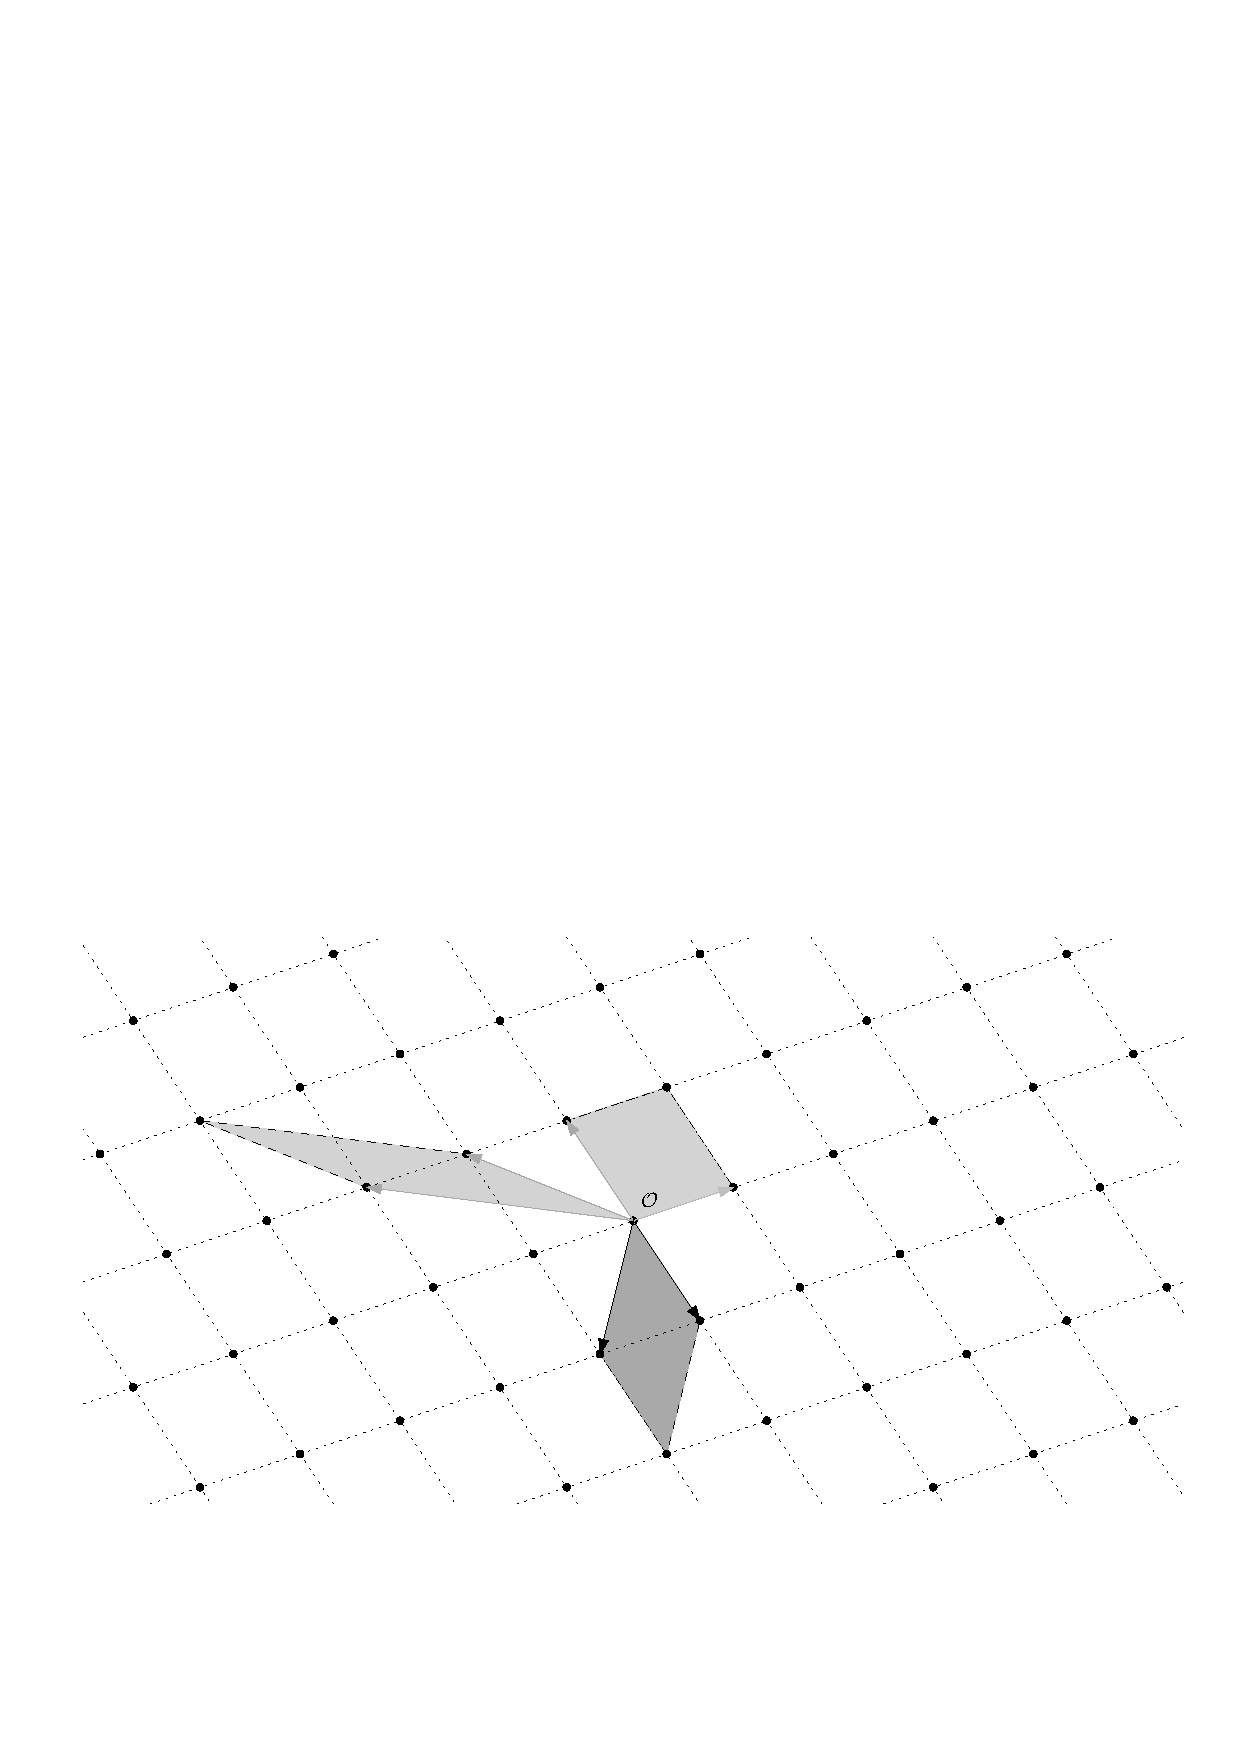
\includegraphics[width=0.8\linewidth]{./assets/lattice-volume.pdf}
\end{center}

\tiny Picture Credit: Joop van de Pol
\end{frame}

\begin{frame}[label={sec:orga701467}]{Gaussian Heuristic}
\begin{itemize}
\item The Gaussian heuristic predicts that the number \(|\Lambda \cap \mathcal{B}|\) of lattice points inside a measurable body \(\mathcal{B} \subset \RR^d\) is approximately equal to \(\Vol(\mathcal{B}) / \Vol(\Lambda)\).
\item Applied to Euclidean \(d\)-balls, this means that a shortest vector in a lattice has expected norm \[λ_1(Λ) ≈ \textnormal{GH}(d) \cdot \mathsf{Vol}(\Lambda)^{1/d} \approx \sqrt{\frac{d}{2 π e}} \cdot \mathsf{Vol}(\Lambda)^{1/d} .\]
\end{itemize}

\begin{block}{Unusually Shortest Vector}
When \(λ_1(Λ) \ll \sqrt{\frac{d}{2 π e}} \cdot \mathsf{Vol}(\Lambda)^{1/d}\).
\end{block}
\end{frame}

\begin{frame}[label={sec:org09cd63f}]{Length of Gram--Schmidt Vectors}
It will be useful to consider the lengths of the Gram--Schmidt vectors.

The vector \(\vec{b}^*_i\) is the orthogonal projection of \(\vec{b}_i\) to the space spanned by the vectors \(\vec{b}_0, \ldots, \vec{b}_{i-1}\).

\begin{columns}
\begin{column}{0.45\columnwidth}
\vspace{1em}

Informally, this means taking out the contributions in the directions of previous vectors  \(\vec{b}_0, \ldots, \vec{b}_{i-1}\).

\vspace{1em}

We have \(\Vol(\Lambda) = \prod_{i=0}^{d-1} \|\vec{b}_{i}^{*}\|\).
\end{column}

\begin{column}{0.45\columnwidth}
\begin{tikzpicture}
\pgfplotsset{width=\textwidth, height=0.6\textwidth}
\draw[->] (0,0) -- (3,1);
\node[] at (3.2,1.2) {$\vec{b}_0$};
\only<1>{\draw[->] (0,0) -- (1,2);}
\only<1>{\node[] at (1.2,2.2) {$\vec{b}_1$};}
\only<2>{\draw[->,color=lightgray] (0,0) -- (1,2);}
\only<2>{\node[color=lightgray] at (1.2,2.2) {$\vec{b}_1$};}
\only<2>{\draw[->,gray] (0,0) -- (-0.5,1.5);}
\only<2>{\node[] at (-0.3,1.7) {$\vec{b}^*_1$};}
\only<1>{\node[] at (-0.3,1.7) {\phantom{$\vec{b}^*_1$}};}
\end{tikzpicture}
\end{column}
\end{columns}
\end{frame}

\begin{frame}[label={sec:org4d31714},fragile]{Example}
 \lstset{language=Python,label= ,caption= ,captionpos=b,numbers=none}
\begin{lstlisting}
A = IntegerMatrix.random(120, "qary", k=60, bits=20)[::-1]
M = GSO.Mat(A, update=True)
line([(i,log(r_, 2)/2) for i, r_ in enumerate(M.r())], **plot_kwds)
\end{lstlisting}

\begin{center}
\includegraphics[width=.9\linewidth]{cache/log-gso-input.png}
\end{center}
\end{frame}

\begin{frame}[label={sec:orgcdeb638},fragile]{Example - LLL}
 \lstset{language=Python,label= ,caption= ,captionpos=b,numbers=none}
\begin{lstlisting}
A = LLL.reduction(A)
M = GSO.Mat(A, update=True)
line([(i,log(r_, 2)/2) for i, r_ in enumerate(M.r())], **plot_kwds)
\end{lstlisting}

\begin{center}
\includegraphics[width=.9\linewidth]{./cache/log-gso-lll.png}
\end{center}
\end{frame}

\begin{frame}[label={sec:org9f92158}]{LLL: Definitions / Intuition}
\begin{columns}
\begin{column}{0.6\columnwidth}
\begin{itemize}
\item Let \(\{\vec{b}_0, \dots, \vec{b}_{d-1} \}\) be a basis \(\mat{B}\) for a lattice \(\Lambda\).
\item Denote by \(\{ \vec{b}_0^*, \dots, \vec{b}_{d-1}^*\}\) be the corresponding Gram--Schmidt orthogonal basis and for \(0 \le j < i < d\) let \(\mu_{i,j} = \langle \vec{b}_i, \vec{b}_j^* \rangle / \langle \vec{b}_j^*, \vec{b}_j^* \rangle.\)
\item An (ordered) basis is \textbf{LLL reduced} if:
\begin{itemize}
\item It is \textbf{size reduced}, i.e. \[| \mu_{i,j} | \le 1/2 \textnormal{ for } 0 \le j < i < d.\]
\item The \textbf{Lovász condition} holds: for \(1 \le i <d\) and \(\delta \in (1/4, 1)\)
\[ \Vert \vec{b}_i^*\Vert^2 \ge \left(\delta - \mu_{i,i-1}^2\right) \cdot \Vert \vec{b}_{i-1}^* \Vert^2 \]
\end{itemize}
\end{itemize}
\end{column}

\begin{column}{0.4\columnwidth}
\begin{block}{Intuition for Lovász Condition}
\begin{itemize}
\item We know that \(\det(\Lambda) = \prod_i \vec{b}_i^*\) is invariant.
\item If \(\vec{b}_i^*\) is not much smaller than \(\vec{b}_{i-1}^*\) then we "moved" some of the contributions of \(\vec{b}_j^*\) for \(j<i\) to \(\vec{b}_i^*\).
\item Since \(\vec{b}_0 = \mathbf{b}_0^*\) this means that we are also producing a shorter vector \(\vec{b}_0\).
\end{itemize}
\end{block}
\end{column}
\end{columns}
\end{frame}

\begin{frame}[label={sec:org223adf0}]{LLL: Algorithm / Guarantees}
\begin{columns}
\begin{column}{0.5\columnwidth}
\begin{algorithm}[H]
  \KwData{Lattice basis \(\mat{B}\)}
  \KwData{Parameter \(\delta \in (1/4,1)\)}
  \(k \gets 1\)\;
  \SetKwFor{MRepeat}{repeat}{}{}
  \MRepeat{until \(k \geq d\)}{
    \For{\(j \gets k-1\) \KwTo{} 0}{
        \(\vec{b}_{k} \gets \vec{b}_{k} - \lfloor \mu_{k,j} \rceil \cdot \vec{b}_{j}\)\;              
    }
    \eIf{\( \| \vec{b}^{*}_{k} \|^{2} \geq (\delta - \mu_{k,j-1}^2) \cdot \|\vec{b}^{*}_{k-1}\|^{2}\)}{
      \(k \gets k + 1\)\;
    }{
      swap \(\vec{b}_{k}\) and \(\vec{b}_{k-1}\)\;
      \(k\gets k - 1\)\;
    }
  }
\end{algorithm}
\end{column}

\begin{column}{0.5\columnwidth}
An LLL-reduced basis satisfies:
\begin{itemize}
\item \(\Vert \vec{b}_0 \Vert \le 2^{(d-1)/4} \cdot \Vol(\Lambda)^{1/d}\) and
\item \(\Vert \vec{b}_0 \Vert \le 2^{(d-1)/2} \cdot \Vert \lambda_{1}(\Lambda) \Vert\).
\end{itemize}
\end{column}
\end{columns}
\end{frame}

\begin{frame}[label={sec:orgadd793e}]{GSA}
\begin{center}
\includegraphics[width=.9\linewidth]{cache/log-gso-bkz-40.png}
\end{center}

\textbf{Geometric Series Assumption:} The shape after lattice reduction is a line with a flatter slope as lattice reduction gets stronger.\footfullcite{STACS:Schnorr03}
\end{frame}

\begin{frame}[label={sec:org43e5b8d}]{Strong Lattice Reduction: BKZ Algorithm (Block 0)}
\centering
\(\left(\begin{array}{ccccccccc}
\phantom{\pi_0(\vec{b}_0)} &
\phantom{\pi_0(\vec{b}_1)} &
\phantom{\pi_0(\vec{b}_2)} &
\phantom{\pi_0(\vec{b}_3)} &
\phantom{\pi_0(\vec{b}_4)} &
\phantom{\pi_0(\vec{b}_5)} &
\phantom{\pi_0(\vec{b}_6)} &
\phantom{\pi_0(\vec{b}_7)} & 
\\
\\
\\
\only<1-2>{\vec{b}_{0}}\only<3->{{\color{LightRed}\vec{b}_{0}}} &
          {\vec{b}_{1}}                                         &
          {\vec{b}_{2}}                                         &
          {\vec{b}_{3}}                                         &
          {\vec{b}_{4}}                                         &
          {\vec{b}_{5}}                                         &
          {\vec{b}_{6}}                                         &
          {\vec{b}_{7}}                                         &
\ldots\\
\\
\\
\\
\end{array}\right)\)
\begin{tikzpicture}[remember picture, overlay]
\tikzset{shift={(current page.center)},yshift=-1.5cm}
\node[] at (0,0) (origin) {};
{\color{DarkBlue} %
  \draw (-5.1,3.0) -- (-5.1,2.0) {};
  \draw (-5.1,1.0) -- (-5.1,0.0) {};
  \draw (0.2,3.0) -- (0.2,2.0) {};
  \draw (0.2,1.0) -- (0.2,0.0) {};
  \draw[decorate,decoration={brace,amplitude=10pt}] (-5.1,3.2) -- (0.2,3.2) node [black,midway,yshift=.6cm]{$\beta = 5$};
  \only<2>{%
    \draw[decorate,decoration={brace,amplitude=10pt}] (0.2,-0.2) -- (-5.1,-0.2) {};
  }
}
\node (oracle) at (-3,-1.8) {
\includegraphics[scale=0.9]{./assets/oracle.png}};
\only<2>{%
  \draw[->] (-4.5,-.8) .. controls (-4.3,-1.4) and (-3.8,-1.6)  .. (-3.5,-1.8);
  \draw[->] (-2.5,-1.8) .. controls (-2.3,-1.7)  and (-2.0,-1.6).. (-2.4,-.8);
}
\node at (5, -2.5) {\tiny{Picture credit: Eamonn Postlethwaite}};
\end{tikzpicture}
\end{frame}

\begin{frame}[label={sec:orgc13847b}]{Strong Lattice Reduction: BKZ Algorithm (Block 1)}
\centering
\(\left(\begin{array}{ccccccccc}
\phantom{\pi_0(\vec{b}_0)} &
\phantom{\pi_0(\vec{b}_1)} &
\phantom{\pi_0(\vec{b}_2)} &
\phantom{\pi_0(\vec{b}_3)} &
\phantom{\pi_0(\vec{b}_4)} &
\phantom{\pi_0(\vec{b}_5)} &
\phantom{\pi_0(\vec{b}_6)} &
\phantom{\pi_0(\vec{b}_7)} & 
\\
\\
\\
{\color{LightRed}\vec{b}_{0}}                                               &
\only<1-2>{\pi_0(\vec{b}_{1})}\only<3->{{\color{LightRed}\pi_{0}(\vec{b}_{1})}} &
          {\pi_0(\vec{b}_{2})}                                                &
          {\pi_0(\vec{b}_{3})}                                                &
          {\pi_0(\vec{b}_{4})}                                                &
          {\pi_0(\vec{b}_{5})}                                                &
          {\vec{b}_{6}}                                                     &
          {\vec{b}_{7}}                                                     &
\ldots\\
\\
\\
\\
\end{array}\right)\)
\begin{tikzpicture}[remember picture, overlay]
\tikzset{shift={(current page.center)},yshift=-1.5cm}
\node[] at (0,0) (origin) {};
{\color{DarkBlue} %
  \draw (-3.8,3.0) -- (-3.8,2.0) {};
  \draw (-3.8,1.0) -- (-3.8,0.0) {};
  \draw (1.4,3.0) -- (1.4,2.0) {};
  \draw (1.4,1.0) -- (1.4,0.0) {};
  \draw[decorate,decoration={brace,amplitude=10pt}] (-3.8,3.2) -- (1.4,3.2) node [black,midway,yshift=.6cm]{$\beta = 5$};
  \only<2>{%
    \draw[decorate,decoration={brace,amplitude=10pt}] (1.4,-0.2) -- (-3.8,-0.2) {};
  }
}
\node (oracle) at (-3,-1.8) {
\includegraphics[scale=0.9]{./assets/oracle.png}};
\only<2>{%
  \draw[->] (-3.8,-.8) .. controls (-3.7,-1.6) and (-3.6,-1.6)  .. (-3.5,-1.8);
  \draw[->] (-2.5,-1.8) .. controls (-2.0,-1.7)  and (-1.4,-1.6).. (-1.2,-.8);
}
\node at (2.5, -2) {\(\pi_{i}(\vec{v})\): project \(\vec{v}\) orthogonally to \(\vec{b}_{0}, \ldots, \vec{b}_{i}\)};
\end{tikzpicture}
\end{frame}

\begin{frame}[label={sec:org4e999fa}]{BKZ Algorithm}
\begin{algorithm}[H]
  \KwData{LLL-reduced lattice basis \(\mat{B}\)}
  \KwData{block size \(\beta\)}
  \SetKwFor{MRepeat}{repeat}{}{}
  \MRepeat{until no more change}{
    \For{\(\kappa \gets 0\) \KwTo{} \(d-1\)}{
        LLL  on local projected block \([\kappa,\ldots,\kappa+\beta-1]\)\; 
        \(\vec{v} \gets \) find shortest vector in local projected block \([\kappa,\ldots,\kappa+\beta-1]\)\;
        insert $\vec{v}$ into $\vec{B}$\;
    }
  }
\end{algorithm}
\end{frame}

\begin{frame}[label={sec:orged69652}]{Quality: Guarantees}
\begin{columns}[t]
\begin{column}{0.50\columnwidth}
\textbf{BKZ}

\begin{itemize}
\item \(\|\vec b_{0}\| \leq \sqrt{\gamma_{\beta}}^{\frac{d-1}{\beta-1} + 1} \cdot {\Vol(\Lambda)}^{1/d}\) and
\item \(\|\vec b_{0}\| \leq \gamma_{\beta}^{\frac{d-1}{\beta-1}} \cdot \lambda_{1}(\Lambda)\)
\end{itemize}
\end{column}

\begin{column}{0.50\columnwidth}
\textbf{Slide}

\begin{itemize}
\item \(\|\vec b_{0}\| \leq \sqrt{(1+\epsilon)\cdot \gamma_{\beta}}^{\frac{d-1}{\beta-1}} \cdot {\Vol(\Lambda)}^{1/d}\) and

\item \(\|\vec b_{0}\| \leq {\left((1+\epsilon)\cdot \gamma_{\beta}\right)}^{\frac{d-\beta}{\beta-1}} \cdot \lambda_{1}(\Lambda)\)
\end{itemize}
\end{column}
\end{columns}

\begin{table}[htbp]
\centering
\begin{tabular}{rrrrrrrrrr}
\toprule
\(\beta\) & 2 & 3 & 4 & 5 & 6 & 7 & 8 & 24 & \(n\)\\
\midrule
\(\gamma_{\beta}^{\frac{1}{2(\beta-1)}}\) & 1.074 & 1.059 & 1.059 & 1.053 & 1.052 & 1.050 & 1.050 & 1.031 & \(\leq \sqrt{2} \GH(n)\)\\
\bottomrule
\end{tabular}
\caption{Hermite’s constant \(\gamma_{\beta}\) in dimension \(\beta\).}

\end{table}

\scriptsize

\fullcite{SchEuc94}

\fullcite{STOC:GamNgu08}
\end{frame}

\begin{frame}[label={sec:org3941cb1}]{Quality: Average I}
\begin{columns}[t]
\begin{column}{0.50\columnwidth}
\textbf{BKZ}

\begin{itemize}
\item \(\|\vec b_{0}\| \approx {\delta_{\beta}}^{{d-1}} \cdot {\Vol(\Lambda)}^{1/d}\) or
\item \(\|\vec b_{0}\| \approx {\delta_{\beta}}^{2\cdot{(d-1)}} \cdot \lambda_{1}(\Lambda)\)
\end{itemize}
\end{column}

\begin{column}{0.50\columnwidth}
\textbf{Slide}

\begin{itemize}
\item \(\|\vec b_{0}\| \approx {\delta_{\beta}}^{{d-1}} \cdot {\Vol(\Lambda)}^{1/d}\) or

\item \(\|\vec b_{0}\| \approx {\delta_{\beta}}^{2\cdot{(d-\beta)}} \cdot \lambda_{1}(\Lambda)\)
\end{itemize}
\end{column}
\end{columns}

\begin{center}
\begin{tabular}{rrrrrrrr}
\toprule
\(\beta\) & 2 & 5 & 24 & 50 & 100 & 200 & 500\\
\midrule
\(\delta\)\textsubscript{\(\beta\)} & 1.0219 & 1.0186 & 1.0142 & 1.0121 & 1.0096 & 1.0063 & 1.0034\\
\bottomrule
\end{tabular}

\end{center}

\begin{itemize}
\item We have \(\delta_{\beta} = \GH(\beta)^{1/(\beta-1)}\) for \(\beta > 50\).
\item The slope under the \textbf{Geometric Series Assumption} is
\end{itemize}
\[\alpha_{\beta} = \delta_{\beta}^{-2}.\]
\end{frame}

\begin{frame}[label={sec:org7d9a47e}]{Quality: Average II}
\tikzset{external/export=true}
\tikzsetnextfilename{root-hermite-factor}
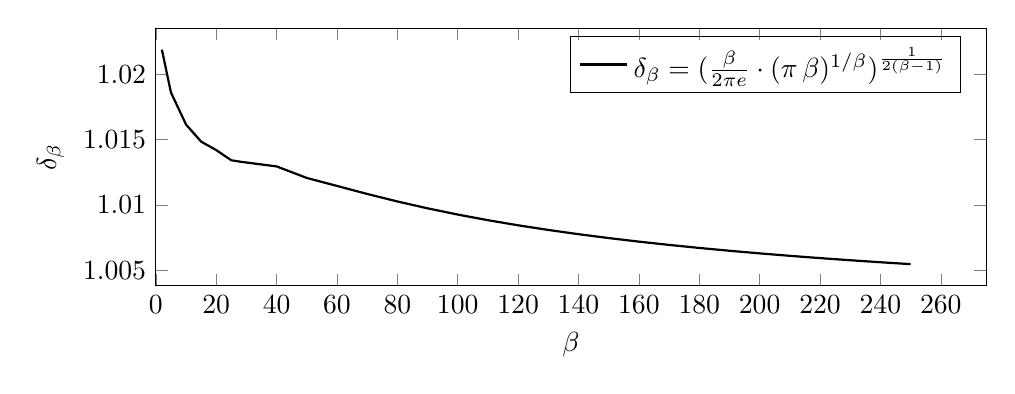
\begin{tikzpicture}
\pgfplotsset{width=\textwidth, height=0.4\textwidth}

\begin{axis}[xmin=0,xlabel={$\beta$},ylabel={$\delta_{\beta}$},legend pos=north east, legend style={fill=none},  yticklabel style={/pgf/number format/fixed, /pgf/number format/precision=4}]
         	
\addplot[black, thick] coordinates {
( 2, 1.02190) ( 5, 1.01862) (10, 1.01616) (15, 1.01485) 
(20, 1.01420) (25, 1.01342) (28, 1.01331) (40, 1.01295)
(50, 1.01206486355485) (60, 1.01145310214785) (70, 1.01083849117278)
(80, 1.01026264533039) (90, 1.00973613406057) (100, 1.00925872103633)
(110, 1.00882653150498) (120, 1.00843474281592) (130, 1.00807860284815)
(140, 1.00775378902354) (150, 1.00745650119215) (160, 1.00718344897388)
(170, 1.00693180103572) (180, 1.00669912477197) (190, 1.00648332800111)
(200, 1.00628260691082) (210, 1.00609540127612) (220, 1.00592035664374)
(230, 1.00575629268952) (240, 1.00560217684407) (250, 1.00545710232739)
};
\addlegendentry{$\delta_{\beta} = (\frac{\beta}{2\pi e} \cdot (\pi\, \beta)^{1/\beta} )^{\frac{1}{2(\beta-1)}}$};

\end{axis}
\end{tikzpicture}
\tikzset{external/export=false}

\scriptsize{

\fullcite{PhD:Chen13}

}
\end{frame}

\begin{frame}[allowframebreaks]{Behaviour in Practice: BKZ-60 in Dimension 180}
\tikzset{external/export=true}

\vspace{-0.8em}
\tikzsetnextfilename{bkz-loggso-evolution0-lll}
\begin{tikzpicture}
  \begin{axis}[ylabel=\(\log_2(\|\vec{b}_i^*\|)\),xlabel=\(i\),legend pos=north east,height=0.5\textwidth,ymin=3,ymax=16,xmin=0,xmax=180]
    \addplot+[black] table [x=i, y=gsa, col sep=comma]{data/bkz-60-180-loggso-evolution.csv};
    \addlegendentry{GSA};
    \addplot+[] table [x=i, y=lll, col sep=comma]{data/bkz-60-180-loggso-evolution.csv};
    \addlegendentry{LLL};
  \end{axis}
\end{tikzpicture}

\framebreak

\tikzsetnextfilename{bkz-loggso-evolution1}
\begin{tikzpicture}
  \begin{axis}[ylabel=\(\log_2(\|\vec{b}_i^*\|)\),xlabel=\(i\),legend pos=north east,height=0.5\textwidth,ymin=3,ymax=16,xmin=0,xmax=180]
    \addplot+[black] table [x=i, y=gsa, col sep=comma]{data/bkz-60-180-loggso-evolution.csv};
    \addlegendentry{GSA};
    \addplot+[] table [x=i, y=tour0, col sep=comma]{data/bkz-60-180-loggso-evolution.csv};
    \addlegendentry{Tour 0};
  \end{axis}
\end{tikzpicture}

\framebreak

\tikzsetnextfilename{bkz-loggso-evolution2}
\begin{tikzpicture}
  \begin{axis}[ylabel=\(\log_2(\|\vec{b}_i^*\|)\),xlabel=\(i\),legend pos=north east,height=0.5\textwidth,ymin=3,ymax=16,xmin=0,xmax=180]
    \addplot+[black] table [x=i, y=gsa, col sep=comma]{data/bkz-60-180-loggso-evolution.csv};
    \addlegendentry{GSA};
    \addplot+[] table [x=i, y=tour1, col sep=comma]{data/bkz-60-180-loggso-evolution.csv};
    \addlegendentry{Tour 1};
  \end{axis}
\end{tikzpicture}


\framebreak

\tikzsetnextfilename{bkz-loggso-evolution3}
\begin{tikzpicture}
  \begin{axis}[ylabel=\(\log_2(\|\vec{b}_i^*\|)\),xlabel=\(i\),legend pos=north east,height=0.5\textwidth,ymin=3,ymax=16,xmin=0,xmax=180]
    \addplot+[black] table [x=i, y=gsa, col sep=comma]{data/bkz-60-180-loggso-evolution.csv};
    \addlegendentry{GSA};
    \addplot+[] table [x=i, y=tour2, col sep=comma]{data/bkz-60-180-loggso-evolution.csv};
    \addlegendentry{Tour 2};
  \end{axis}
\end{tikzpicture}

\framebreak

\tikzsetnextfilename{bkz-loggso-evolution4}
\begin{tikzpicture}
  \begin{axis}[ylabel=\(\log_2(\|\vec{b}_i^*\|)\),xlabel=\(i\),legend pos=north east,height=0.5\textwidth,ymin=3,ymax=16,xmin=0,xmax=180]
    \addplot+[black] table [x=i, y=gsa, col sep=comma]{data/bkz-60-180-loggso-evolution.csv};
    \addlegendentry{GSA};
    \addplot+[] table [x=i, y=tour3, col sep=comma]{data/bkz-60-180-loggso-evolution.csv};
    \addlegendentry{Tour 3};
  \end{axis}
\end{tikzpicture}

\framebreak

\tikzsetnextfilename{bkz-loggso-evolution5}
\begin{tikzpicture}
  \begin{axis}[ylabel=\(\log_2(\|\vec{b}_i^*\|)\),xlabel=\(i\),legend pos=north east,height=0.5\textwidth,ymin=3,ymax=16,xmin=0,xmax=180]
    \addplot+[black] table [x=i, y=gsa, col sep=comma]{data/bkz-60-180-loggso-evolution.csv};
    \addlegendentry{GSA};
    \addplot+[] table [x=i, y=tour4, col sep=comma]{data/bkz-60-180-loggso-evolution.csv};
    \addlegendentry{Tour 4};
  \end{axis}
\end{tikzpicture}

\framebreak

\tikzsetnextfilename{bkz-loggso-evolution6}
\begin{tikzpicture}
  \begin{axis}[ylabel=\(\log_2(\|\vec{b}_i^*\|)\),xlabel=\(i\),legend pos=north east,height=0.5\textwidth,ymin=3,ymax=16,xmin=0,xmax=180]
    \addplot+[black] table [x=i, y=gsa, col sep=comma]{data/bkz-60-180-loggso-evolution.csv};
    \addlegendentry{GSA};
    \addplot+[] table [x=i, y=tour5, col sep=comma]{data/bkz-60-180-loggso-evolution.csv};
    \addlegendentry{Tour 5};
  \end{axis}
\end{tikzpicture}

\framebreak

\tikzsetnextfilename{bkz-loggso-evolution7}
\begin{tikzpicture}
  \begin{axis}[ylabel=\(\log_2(\|\vec{b}_i^*\|)\),xlabel=\(i\),legend pos=north east,height=0.5\textwidth,ymin=3,ymax=16,xmin=0,xmax=180]
    \addplot+[black] table [x=i, y=gsa, col sep=comma]{data/bkz-60-180-loggso-evolution.csv};
    \addlegendentry{GSA};
    \addplot+[] table [x=i, y=tour6, col sep=comma]{data/bkz-60-180-loggso-evolution.csv};
    \addlegendentry{Tour 6};
  \end{axis}
\end{tikzpicture}

\framebreak

\tikzsetnextfilename{bkz-loggso-evolution8}
\begin{tikzpicture}
  \begin{axis}[ylabel=\(\log_2(\|\vec{b}_i^*\|)\),xlabel=\(i\),legend pos=north east,height=0.5\textwidth,ymin=3,ymax=16,xmin=0,xmax=180]
    \addplot+[black] table [x=i, y=gsa, col sep=comma]{data/bkz-60-180-loggso-evolution.csv};
    \addlegendentry{GSA};
    \addplot+[] table [x=i, y=tour7, col sep=comma]{data/bkz-60-180-loggso-evolution.csv};
    \addlegendentry{Tour 7};
  \end{axis}
\end{tikzpicture}


\framebreak

\tikzsetnextfilename{bkz-loggso-evolution9}
\begin{tikzpicture}
  \begin{axis}[ylabel=\(\log_2(\|\vec{b}_i^*\|)\),xlabel=\(i\),legend pos=north east,height=0.5\textwidth,ymin=3,ymax=16,xmin=0,xmax=180]
    \addplot+[black] table [x=i, y=simulator, col sep=comma]{data/bkz-60-180-loggso-evolution.csv};
    \addlegendentry{Simulator};
    \addplot+[] table [x=i, y=tour7, col sep=comma]{data/bkz-60-180-loggso-evolution.csv};
    \addlegendentry{Tour 7};
  \end{axis}
\end{tikzpicture}

\tikzset{external/export=false}
\end{frame}

\begin{frame}[label={sec:org549ef04},fragile]{Try it at Home}
 \lstset{language=Python,label= ,caption= ,captionpos=b,numbers=none}
\begin{lstlisting}
from fpylll import *
from fpylll.algorithms.bkz2 import BKZReduction as BKZ2
A = IntegerMatrix.random(180, "qary", k=90, bits=20)
bkz = BKZ2(A)
bkz(BKZ.EasyParam(block_size=60))
\end{lstlisting}

\begin{description}
\item[{\url{https://github.com/fplll/fplll}}] C++ library
\item[{\url{https://github.com/fplll/fpylll}}] Python interface
\item[{\url{https://sagemath.org}}] FPyLLL is in Sage
\item[{\url{https://sagecell.sagemath.org/}}] Sage in your browser
\item[{\url{https://cocalc.com/}}] Sage worksheets in your browser
\end{description}
\end{frame}

\begin{frame}[label={sec:org288da69}]{Success Condition for uSVP (Expectation)}
Can decide that \(\Lambda = \Lambda(\mat{B})\) has unusually short vector when

\vspace{1em}

\begin{columns}[t]
\begin{column}{0.45\columnwidth}
\textbf{BKZ}

\begin{itemize}
\item \({\delta_{\beta}}^{2\,(d-1)} \cdot \lambda_{1}(\Lambda) < {\delta_{\beta}}^{d-1} \cdot {\Vol(\Lambda)}^{1/d}\)

\item \(\lambda_{1}(\Lambda) < {\delta_{\beta}}^{-d+1} \cdot {\Vol(\Lambda)}^{1/d}\)
\end{itemize}
\end{column}


\begin{column}{0.45\columnwidth}
\textbf{Slide}

\begin{itemize}
\item \({\delta_{\beta}}^{2\cdot(d-\beta)} \cdot \lambda_{1}(\Lambda) < {\delta_{\beta}}^{d-1} \cdot {\Vol(\Lambda)}^{1/d}\)
\item \(\lambda_{1}(\Lambda) < {\delta_{\beta}}^{\alert<3->{2\beta-d-1}} \cdot {\Vol(\Lambda)}^{1/d}\)
\end{itemize}

\pause
\end{column}
\end{columns}

\begin{block}{“2016 Estimate”}
\[\alert<4>{\sqrt{\beta/d}} \cdot \norm{(\vec{e} \mid \vec{s} \mid 1)} \approx \sqrt{\beta} \cdot \sigma < \delta_{\beta}^{\alert<3->{2\beta-d-1}} \cdot {\Vol(\Lambda)}^{1/d}\]

\scriptsize{

\fullcite{USENIX:ADPS16}

}
\end{block}
\end{frame}

\begin{frame}[label={sec:org4600094}]{Success Condition for uSVP (Expectation)}
\vspace{-2.6em}

\tikzset{external/export=true}
\tikzsetnextfilename{usvp-success-expectation}
\begin{tikzpicture}
\begin{axis}[/pgf/number format/.cd,fixed,ymin = 1,legend pos=north east,legend style={fill=white}, xlabel=,ylabel=$\log_2(\norm \cdot)$,width=\columnwidth, height=0.4\columnwidth, xmin = 1, xmax = 183,legend cell align=left,ymax=9]
%      \draw[->] (-3,0) -- (4.2,0) node[right] {$x$};
%      \draw[->] (0,-3) -- (0,4.2) node[above] {$y$};
\addplot[domain=1:183,smooth,variable=\x,black] plot ({\x},{log2(1.01170246711949^(-2*(\x-1)+183)*54.5751087741536)});
\addlegendentry{GSA for $\norm{\vec b_i^*}$}

\addplot[domain=1:183,samples=1000, smooth,variable=\x,darkgray,dotted,thick] plot ({\x},{log2( 3.19153824321146 * sqrt(183 - \x + 1) )});

\addlegendentry{length of projection of $(\vec{e},\vec{s},1)$}

\draw[dashed] (127,1) -- (127,820) node[pos = 0.06, right] {$d-\beta$};
\end{axis}
\end{tikzpicture}
\tikzset{external/export=false}

\scriptsize{

\fullcite{USENIX:ADPS16}  \phantom{Foo Foo Foo Foo Foo Foo Foo Foo Foo Foo Foo Foo Foo}

}
\end{frame}

\begin{frame}[label={sec:orge74144a}]{Success Condition for uSVP (Observed)}
\tikzset{external/export=true}
\tikzsetnextfilename{usv-success-observation}
\begin{tikzpicture}
\begin{axis}[/pgf/number format/.cd,fixed, ymin = 1,legend pos=north east, xlabel= ,ylabel=$\log_2(\norm \cdot)$,width=\columnwidth, height=0.4\columnwidth, xmin = 1, xmax = 183,legend cell align=left,ymax=9]
%      \draw[->] (-3,0) -- (4.2,0) node[right] {$x$};
%      \draw[->] (0,-3) -- (0,4.2) node[above] {$y$};

\addplot[gray,thick,x filter/.code={\pgfmathparse{\pgfmathresult+1.0}}] coordinates {
   (  0,  8.78) (  1,  8.78) (  2,  8.77) (  3,  8.72) (  4,  8.71) (  5,  8.69) (  6,  8.66) (  7,  8.63) (  8,  8.62) (  9,  8.59) ( 10,  8.54) ( 11,  8.53) ( 12,  8.51) ( 13,  8.47) ( 14,  8.43) ( 15,  8.39) ( 16,  8.36) ( 17,  8.34) ( 18,  8.30) ( 19,  8.28) ( 20,  8.24) ( 21,  8.20) ( 22,  8.16) ( 23,  8.13) ( 24,  8.10) ( 25,  8.07) ( 26,  8.04) ( 27,  7.99) ( 28,  7.96) ( 29,  7.94) ( 30,  7.91) ( 31,  7.88) ( 32,  7.84) ( 33,  7.79) ( 34,  7.76) ( 35,  7.73) ( 36,  7.69) ( 37,  7.65) ( 38,  7.61) ( 39,  7.59) ( 40,  7.55) ( 41,  7.52) ( 42,  7.48) ( 43,  7.44) ( 44,  7.39) ( 45,  7.37) ( 46,  7.33) ( 47,  7.31) ( 48,  7.27) ( 49,  7.24) ( 50,  7.21) ( 51,  7.18) ( 52,  7.15) ( 53,  7.09) ( 54,  7.07) ( 55,  7.03) ( 56,  7.00) ( 57,  6.97) ( 58,  6.95) ( 59,  6.91) ( 60,  6.87) ( 61,  6.83) ( 62,  6.79) ( 63,  6.74) ( 64,  6.72) ( 65,  6.67) ( 66,  6.64) ( 67,  6.62) ( 68,  6.59) ( 69,  6.55) ( 70,  6.52) ( 71,  6.46) ( 72,  6.44) ( 73,  6.40) ( 74,  6.38) ( 75,  6.34) ( 76,  6.31) ( 77,  6.28) ( 78,  6.24) ( 79,  6.21) ( 80,  6.15) ( 81,  6.13) ( 82,  6.09) ( 83,  6.06) ( 84,  6.02) ( 85,  6.00) ( 86,  5.97) ( 87,  5.92) ( 88,  5.88) ( 89,  5.86) ( 90,  5.82) ( 91,  5.78) ( 92,  5.75) ( 93,  5.73) ( 94,  5.71) ( 95,  5.66) ( 96,  5.64) ( 97,  5.59) ( 98,  5.55) ( 99,  5.51) (100,  5.47) (101,  5.43) (102,  5.41) (103,  5.36) (104,  5.36) (105,  5.31) (106,  5.28) (107,  5.25) (108,  5.23) (109,  5.18) (110,  5.13) (111,  5.09) (112,  5.04) (113,  5.01) (114,  5.00) (115,  4.96) (116,  4.92) (117,  4.86) (118,  4.83) (119,  4.79) (120,  4.77) (121,  4.72) (122,  4.68) (123,  4.66) (124,  4.63) (125,  4.60) (126,  4.56) (127,  4.52) (128,  4.50) (129,  4.45) (130,  4.43) (131,  4.40) (132,  4.36) (133,  4.34) (134,  4.30) (135,  4.27) (136,  4.24) (137,  4.22) (138,  4.18) (139,  4.16) (140,  4.12) (141,  4.09) (142,  4.06) (143,  4.03) (144,  4.01) (145,  3.95) (146,  3.91) (147,  3.89) (148,  3.85) (149,  3.81) (150,  3.77) (151,  3.75) (152,  3.71) (153,  3.66) (154,  3.62) (155,  3.59) (156,  3.55) (157,  3.51) (158,  3.47) (159,  3.43) (160,  3.39) (161,  3.37) (162,  3.29) (163,  3.27) (164,  3.23) (165,  3.19) (166,  3.13) (167,  3.08) (168,  3.03) (169,  2.99) (170,  2.94) (171,  2.89) (172,  2.84) (173,  2.79) (174,  2.76) (175,  2.72) (176,  2.68) (177,  2.65) (178,  2.61) (179,  2.58) (180,  2.51) (181,  2.54) (182,  2.56) };
\addlegendentry{Average for $\norm{\vec b_i^*}$}

  \addplot[black] coordinates {(  1, 5.453) (  2, 5.450) (  3, 5.449) (  4, 5.446) (  5, 5.442) (  6, 5.434) (  7, 5.430) (  8, 5.428) (  9, 5.424) ( 10, 5.416) ( 11, 5.411) ( 12, 5.407) ( 13, 5.402) ( 14, 5.397) ( 15, 5.392) ( 16, 5.388) ( 17, 5.385) ( 18, 5.383) ( 19, 5.380) ( 20, 5.375) ( 21, 5.366) ( 22, 5.358) ( 23, 5.355) ( 24, 5.352) ( 25, 5.350) ( 26, 5.345) ( 27, 5.341) ( 28, 5.336) ( 29, 5.332) ( 30, 5.327) ( 31, 5.322) ( 32, 5.317) ( 33, 5.312) ( 34, 5.307) ( 35, 5.305) ( 36, 5.299) ( 37, 5.296) ( 38, 5.290) ( 39, 5.285) ( 40, 5.279) ( 41, 5.276) ( 42, 5.273) ( 43, 5.267) ( 44, 5.261) ( 45, 5.255) ( 46, 5.252) ( 47, 5.248) ( 48, 5.241) ( 49, 5.237) ( 50, 5.233) ( 51, 5.230) ( 52, 5.222) ( 53, 5.217) ( 54, 5.209) ( 55, 5.206) ( 56, 5.204) ( 57, 5.197) ( 58, 5.190) ( 59, 5.182) ( 60, 5.175) ( 61, 5.166) ( 62, 5.157) ( 63, 5.151) ( 64, 5.144) ( 65, 5.139) ( 66, 5.132) ( 67, 5.123) ( 68, 5.117) ( 69, 5.111) ( 70, 5.108) ( 71, 5.105) ( 72, 5.099) ( 73, 5.087) ( 74, 5.082) ( 75, 5.078) ( 76, 5.074) ( 77, 5.063) ( 78, 5.057) ( 79, 5.052) ( 80, 5.041) ( 81, 5.026) ( 82, 5.021) ( 83, 5.013) ( 84, 5.001) ( 85, 4.996) ( 86, 4.988) ( 87, 4.970) ( 88, 4.963) ( 89, 4.956) ( 90, 4.949) ( 91, 4.941) ( 92, 4.937) ( 93, 4.929) ( 94, 4.925) ( 95, 4.915) ( 96, 4.909) ( 97, 4.898) ( 98, 4.887) ( 99, 4.875) (100, 4.860) (101, 4.846) (102, 4.830) (103, 4.824) (104, 4.815) (105, 4.806) (106, 4.796) (107, 4.791) (108, 4.780) (109, 4.759) (110, 4.750) (111, 4.741) (112, 4.729) (113, 4.714) (114, 4.699) (115, 4.685) (116, 4.680) (117, 4.668) (118, 4.659) (119, 4.651) (120, 4.641) (121, 4.628) (122, 4.619) (123, 4.605) (124, 4.590) (125, 4.577) (126, 4.567) (127, 4.558) (128, 4.545) (129, 4.537) (130, 4.525) (131, 4.506) (132, 4.489) (133, 4.480) (134, 4.471) (135, 4.459) (136, 4.443) (137, 4.424) (138, 4.412) (139, 4.404) (140, 4.392) (141, 4.374) (142, 4.363) (143, 4.342) (144, 4.316) (145, 4.291) (146, 4.268) (147, 4.242) (148, 4.221) (149, 4.198) (150, 4.174) (151, 4.128) (152, 4.088) (153, 4.073) (154, 4.041) (155, 4.024) (156, 4.006) (157, 3.972) (158, 3.952) (159, 3.929) (160, 3.896) (161, 3.875) (162, 3.797) (163, 3.744) (164, 3.702) (165, 3.675) (166, 3.643) (167, 3.592) (168, 3.552) (169, 3.515) (170, 3.455) (171, 3.411) (172, 3.367) (173, 3.313) (174, 3.246) (175, 3.188) (176, 3.054) (177, 2.936) (178, 2.866) (179, 2.704) (180, 2.464) (181, 2.141) (182, 1.682)};
\addlegendentry{Average for $\norm{\pi_i(\vec e,\vec s,1)}$}

\draw[dashed] (127,1) -- (127,820) node[pos = 0.06, right] {$d-\beta$};
\end{axis}
\end{tikzpicture}
\tikzset{external/export=false}

\scriptsize{

\fullcite{AC:AGVW17}

\fullcite{PKC:PosVir21}

}
\end{frame}

\begin{frame}[label={sec:orgb215440}]{The GSA is a Lie: Tail Shape}
\tikzset{external/export=true}
\tikzsetnextfilename{gsa-comparison}
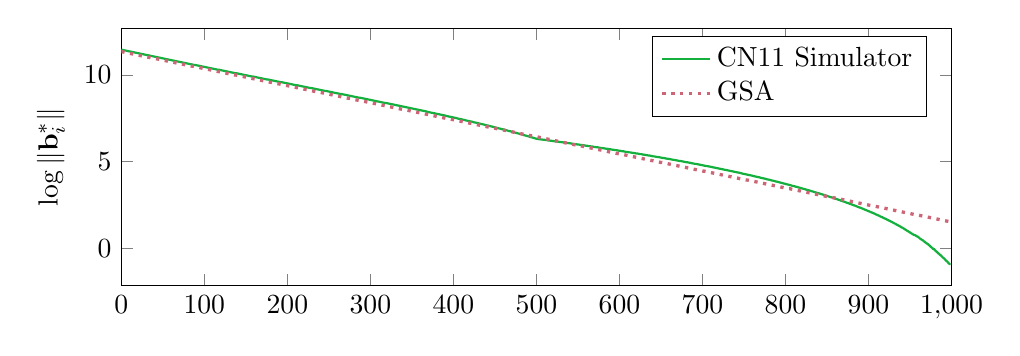
\begin{tikzpicture}
\begin{axis}[xmin=0,xmax=1000,ylabel=\(\log \|\vec{b}_{i}^{*}\|\),legend pos=north east,height=0.4\textwidth]
\addplot+[] coordinates {
(  0, 11.45) (  1, 11.44) (  2, 11.43) (  3, 11.42) (  4, 11.41) (  5, 11.40) (  6, 11.39) 
(  7, 11.38) (  8, 11.37) (  9, 11.36) ( 10, 11.35) ( 11, 11.34) ( 12, 11.33) ( 13, 11.32) 
( 14, 11.31) ( 15, 11.30) ( 16, 11.29) ( 17, 11.28) ( 18, 11.27) ( 19, 11.26) ( 20, 11.25) 
( 21, 11.24) ( 22, 11.23) ( 23, 11.22) ( 24, 11.21) ( 25, 11.20) ( 26, 11.19) ( 27, 11.18) 
( 28, 11.17) ( 29, 11.16) ( 30, 11.15) ( 31, 11.14) ( 32, 11.13) ( 33, 11.12) ( 34, 11.11) 
( 35, 11.10) ( 36, 11.09) ( 37, 11.08) ( 38, 11.07) ( 39, 11.06) ( 40, 11.05) ( 41, 11.04) 
( 42, 11.03) ( 43, 11.02) ( 44, 11.01) ( 45, 11.00) ( 46, 10.99) ( 47, 10.98) ( 48, 10.97) 
( 49, 10.96) ( 50, 10.95) ( 51, 10.94) ( 52, 10.93) ( 53, 10.92) ( 54, 10.91) ( 55, 10.90) 
( 56, 10.89) ( 57, 10.88) ( 58, 10.87) ( 59, 10.86) ( 60, 10.85) ( 61, 10.84) ( 62, 10.83) 
( 63, 10.82) ( 64, 10.81) ( 65, 10.80) ( 66, 10.79) ( 67, 10.78) ( 68, 10.77) ( 69, 10.76) 
( 70, 10.75) ( 71, 10.74) ( 72, 10.73) ( 73, 10.72) ( 74, 10.71) ( 75, 10.70) ( 76, 10.69) 
( 77, 10.68) ( 78, 10.67) ( 79, 10.66) ( 80, 10.65) ( 81, 10.64) ( 82, 10.63) ( 83, 10.62) 
( 84, 10.61) ( 85, 10.60) ( 86, 10.59) ( 87, 10.58) ( 88, 10.57) ( 89, 10.57) ( 90, 10.56) 
( 91, 10.55) ( 92, 10.54) ( 93, 10.53) ( 94, 10.52) ( 95, 10.51) ( 96, 10.50) ( 97, 10.49) 
( 98, 10.48) ( 99, 10.47) (100, 10.46) (101, 10.45) (102, 10.44) (103, 10.43) (104, 10.42) 
(105, 10.41) (106, 10.40) (107, 10.39) (108, 10.38) (109, 10.37) (110, 10.36) (111, 10.35) 
(112, 10.34) (113, 10.33) (114, 10.32) (115, 10.31) (116, 10.30) (117, 10.30) (118, 10.29) 
(119, 10.28) (120, 10.27) (121, 10.26) (122, 10.25) (123, 10.24) (124, 10.23) (125, 10.22) 
(126, 10.21) (127, 10.20) (128, 10.19) (129, 10.18) (130, 10.17) (131, 10.16) (132, 10.15) 
(133, 10.14) (134, 10.13) (135, 10.12) (136, 10.11) (137, 10.10) (138, 10.09) (139, 10.09) 
(140, 10.08) (141, 10.07) (142, 10.06) (143, 10.05) (144, 10.04) (145, 10.03) (146, 10.02) 
(147, 10.01) (148, 10.00) (149,  9.99) (150,  9.98) (151,  9.97) (152,  9.96) (153,  9.95) 
(154,  9.94) (155,  9.93) (156,  9.92) (157,  9.91) (158,  9.91) (159,  9.90) (160,  9.89) 
(161,  9.88) (162,  9.87) (163,  9.86) (164,  9.85) (165,  9.84) (166,  9.83) (167,  9.82) 
(168,  9.81) (169,  9.80) (170,  9.79) (171,  9.78) (172,  9.77) (173,  9.76) (174,  9.75) 
(175,  9.74) (176,  9.73) (177,  9.73) (178,  9.72) (179,  9.71) (180,  9.70) (181,  9.69) 
(182,  9.68) (183,  9.67) (184,  9.66) (185,  9.65) (186,  9.64) (187,  9.63) (188,  9.62) 
(189,  9.61) (190,  9.60) (191,  9.59) (192,  9.58) (193,  9.57) (194,  9.57) (195,  9.56) 
(196,  9.55) (197,  9.54) (198,  9.53) (199,  9.52) (200,  9.51) (201,  9.50) (202,  9.49) 
(203,  9.48) (204,  9.47) (205,  9.46) (206,  9.45) (207,  9.44) (208,  9.43) (209,  9.42) 
(210,  9.41) (211,  9.41) (212,  9.40) (213,  9.39) (214,  9.38) (215,  9.37) (216,  9.36) 
(217,  9.35) (218,  9.34) (219,  9.33) (220,  9.32) (221,  9.31) (222,  9.30) (223,  9.29) 
(224,  9.28) (225,  9.27) (226,  9.26) (227,  9.25) (228,  9.25) (229,  9.24) (230,  9.23) 
(231,  9.22) (232,  9.21) (233,  9.20) (234,  9.19) (235,  9.18) (236,  9.17) (237,  9.16) 
(238,  9.15) (239,  9.14) (240,  9.13) (241,  9.12) (242,  9.11) (243,  9.10) (244,  9.09) 
(245,  9.08) (246,  9.08) (247,  9.07) (248,  9.06) (249,  9.05) (250,  9.04) (251,  9.03) 
(252,  9.02) (253,  9.01) (254,  9.00) (255,  8.99) (256,  8.98) (257,  8.97) (258,  8.96) 
(259,  8.95) (260,  8.94) (261,  8.93) (262,  8.92) (263,  8.91) (264,  8.90) (265,  8.90) 
(266,  8.89) (267,  8.88) (268,  8.87) (269,  8.86) (270,  8.85) (271,  8.84) (272,  8.83) 
(273,  8.82) (274,  8.81) (275,  8.80) (276,  8.79) (277,  8.78) (278,  8.77) (279,  8.76) 
(280,  8.75) (281,  8.74) (282,  8.73) (283,  8.72) (284,  8.71) (285,  8.70) (286,  8.69) 
(287,  8.68) (288,  8.68) (289,  8.67) (290,  8.66) (291,  8.65) (292,  8.64) (293,  8.63) 
(294,  8.62) (295,  8.61) (296,  8.60) (297,  8.59) (298,  8.58) (299,  8.57) (300,  8.56) 
(301,  8.55) (302,  8.54) (303,  8.53) (304,  8.52) (305,  8.51) (306,  8.50) (307,  8.49) 
(308,  8.48) (309,  8.47) (310,  8.46) (311,  8.45) (312,  8.44) (313,  8.43) (314,  8.42) 
(315,  8.41) (316,  8.40) (317,  8.39) (318,  8.38) (319,  8.38) (320,  8.37) (321,  8.36) 
(322,  8.35) (323,  8.34) (324,  8.33) (325,  8.32) (326,  8.31) (327,  8.30) (328,  8.29) 
(329,  8.28) (330,  8.27) (331,  8.26) (332,  8.25) (333,  8.24) (334,  8.23) (335,  8.22) 
(336,  8.21) (337,  8.20) (338,  8.19) (339,  8.18) (340,  8.17) (341,  8.16) (342,  8.15) 
(343,  8.14) (344,  8.13) (345,  8.12) (346,  8.11) (347,  8.10) (348,  8.09) (349,  8.08) 
(350,  8.07) (351,  8.06) (352,  8.05) (353,  8.04) (354,  8.03) (355,  8.02) (356,  8.01) 
(357,  8.00) (358,  7.99) (359,  7.98) (360,  7.97) (361,  7.96) (362,  7.95) (363,  7.94) 
(364,  7.93) (365,  7.92) (366,  7.91) (367,  7.90) (368,  7.88) (369,  7.87) (370,  7.86) 
(371,  7.85) (372,  7.84) (373,  7.83) (374,  7.82) (375,  7.81) (376,  7.80) (377,  7.79) 
(378,  7.78) (379,  7.77) (380,  7.76) (381,  7.75) (382,  7.74) (383,  7.73) (384,  7.72) 
(385,  7.71) (386,  7.70) (387,  7.69) (388,  7.68) (389,  7.67) (390,  7.66) (391,  7.64) 
(392,  7.63) (393,  7.62) (394,  7.61) (395,  7.60) (396,  7.59) (397,  7.58) (398,  7.57) 
(399,  7.56) (400,  7.55) (401,  7.54) (402,  7.53) (403,  7.52) (404,  7.51) (405,  7.49) 
(406,  7.48) (407,  7.47) (408,  7.46) (409,  7.45) (410,  7.44) (411,  7.43) (412,  7.42) 
(413,  7.41) (414,  7.40) (415,  7.38) (416,  7.37) (417,  7.36) (418,  7.35) (419,  7.34) 
(420,  7.33) (421,  7.32) (422,  7.31) (423,  7.30) (424,  7.28) (425,  7.27) (426,  7.26) 
(427,  7.25) (428,  7.24) (429,  7.23) (430,  7.22) (431,  7.20) (432,  7.19) (433,  7.18) 
(434,  7.17) (435,  7.16) (436,  7.15) (437,  7.14) (438,  7.12) (439,  7.11) (440,  7.10) 
(441,  7.09) (442,  7.08) (443,  7.06) (444,  7.05) (445,  7.04) (446,  7.03) (447,  7.02) 
(448,  7.01) (449,  6.99) (450,  6.98) (451,  6.97) (452,  6.96) (453,  6.94) (454,  6.93) 
(455,  6.92) (456,  6.91) (457,  6.90) (458,  6.88) (459,  6.87) (460,  6.86) (461,  6.85) 
(462,  6.83) (463,  6.82) (464,  6.81) (465,  6.80) (466,  6.78) (467,  6.77) (468,  6.76) 
(469,  6.75) (470,  6.73) (471,  6.72) (472,  6.71) (473,  6.69) (474,  6.68) (475,  6.67) 
(476,  6.66) (477,  6.64) (478,  6.63) (479,  6.62) (480,  6.60) (481,  6.59) (482,  6.58) 
(483,  6.56) (484,  6.55) (485,  6.53) (486,  6.52) (487,  6.51) (488,  6.49) (489,  6.48) 
(490,  6.47) (491,  6.45) (492,  6.44) (493,  6.42) (494,  6.41) (495,  6.40) (496,  6.38) 
(497,  6.37) (498,  6.35) (499,  6.34) (500,  6.32) (501,  6.32) (502,  6.31) (503,  6.30) 
(504,  6.30) (505,  6.29) (506,  6.28) (507,  6.28) (508,  6.27) (509,  6.27) (510,  6.26) 
(511,  6.25) (512,  6.25) (513,  6.24) (514,  6.23) (515,  6.23) (516,  6.22) (517,  6.21) 
(518,  6.21) (519,  6.20) (520,  6.19) (521,  6.19) (522,  6.18) (523,  6.17) (524,  6.17) 
(525,  6.16) (526,  6.16) (527,  6.15) (528,  6.14) (529,  6.14) (530,  6.13) (531,  6.12) 
(532,  6.12) (533,  6.11) (534,  6.10) (535,  6.10) (536,  6.09) (537,  6.08) (538,  6.08) 
(539,  6.07) (540,  6.06) (541,  6.06) (542,  6.05) (543,  6.04) (544,  6.03) (545,  6.03) 
(546,  6.02) (547,  6.01) (548,  6.01) (549,  6.00) (550,  5.99) (551,  5.99) (552,  5.98) 
(553,  5.97) (554,  5.97) (555,  5.96) (556,  5.95) (557,  5.95) (558,  5.94) (559,  5.93) 
(560,  5.92) (561,  5.92) (562,  5.91) (563,  5.90) (564,  5.90) (565,  5.89) (566,  5.88) 
(567,  5.88) (568,  5.87) (569,  5.86) (570,  5.85) (571,  5.85) (572,  5.84) (573,  5.83) 
(574,  5.83) (575,  5.82) (576,  5.81) (577,  5.80) (578,  5.80) (579,  5.79) (580,  5.78) 
(581,  5.78) (582,  5.77) (583,  5.76) (584,  5.75) (585,  5.75) (586,  5.74) (587,  5.73) 
(588,  5.72) (589,  5.72) (590,  5.71) (591,  5.70) (592,  5.69) (593,  5.69) (594,  5.68) 
(595,  5.67) (596,  5.67) (597,  5.66) (598,  5.65) (599,  5.64) (600,  5.64) (601,  5.63) 
(602,  5.62) (603,  5.61) (604,  5.61) (605,  5.60) (606,  5.59) (607,  5.58) (608,  5.57) 
(609,  5.57) (610,  5.56) (611,  5.55) (612,  5.54) (613,  5.54) (614,  5.53) (615,  5.52) 
(616,  5.51) (617,  5.51) (618,  5.50) (619,  5.49) (620,  5.48) (621,  5.47) (622,  5.47) 
(623,  5.46) (624,  5.45) (625,  5.44) (626,  5.44) (627,  5.43) (628,  5.42) (629,  5.41) 
(630,  5.40) (631,  5.40) (632,  5.39) (633,  5.38) (634,  5.37) (635,  5.36) (636,  5.36) 
(637,  5.35) (638,  5.34) (639,  5.33) (640,  5.32) (641,  5.31) (642,  5.31) (643,  5.30) 
(644,  5.29) (645,  5.28) (646,  5.27) (647,  5.27) (648,  5.26) (649,  5.25) (650,  5.24) 
(651,  5.23) (652,  5.22) (653,  5.22) (654,  5.21) (655,  5.20) (656,  5.19) (657,  5.18) 
(658,  5.17) (659,  5.17) (660,  5.16) (661,  5.15) (662,  5.14) (663,  5.13) (664,  5.12) 
(665,  5.11) (666,  5.11) (667,  5.10) (668,  5.09) (669,  5.08) (670,  5.07) (671,  5.06) 
(672,  5.05) (673,  5.05) (674,  5.04) (675,  5.03) (676,  5.02) (677,  5.01) (678,  5.00) 
(679,  4.99) (680,  4.98) (681,  4.97) (682,  4.97) (683,  4.96) (684,  4.95) (685,  4.94) 
(686,  4.93) (687,  4.92) (688,  4.91) (689,  4.90) (690,  4.89) (691,  4.88) (692,  4.88) 
(693,  4.87) (694,  4.86) (695,  4.85) (696,  4.84) (697,  4.83) (698,  4.82) (699,  4.81) 
(700,  4.80) (701,  4.79) (702,  4.78) (703,  4.77) (704,  4.76) (705,  4.75) (706,  4.75) 
(707,  4.74) (708,  4.73) (709,  4.72) (710,  4.71) (711,  4.70) (712,  4.69) (713,  4.68) 
(714,  4.67) (715,  4.66) (716,  4.65) (717,  4.64) (718,  4.63) (719,  4.62) (720,  4.61) 
(721,  4.60) (722,  4.59) (723,  4.58) (724,  4.57) (725,  4.56) (726,  4.55) (727,  4.54) 
(728,  4.53) (729,  4.52) (730,  4.51) (731,  4.50) (732,  4.49) (733,  4.48) (734,  4.47) 
(735,  4.46) (736,  4.45) (737,  4.44) (738,  4.43) (739,  4.42) (740,  4.41) (741,  4.40) 
(742,  4.39) (743,  4.38) (744,  4.37) (745,  4.36) (746,  4.35) (747,  4.34) (748,  4.32) 
(749,  4.31) (750,  4.30) (751,  4.29) (752,  4.28) (753,  4.27) (754,  4.26) (755,  4.25) 
(756,  4.24) (757,  4.23) (758,  4.22) (759,  4.21) (760,  4.20) (761,  4.18) (762,  4.17) 
(763,  4.16) (764,  4.15) (765,  4.14) (766,  4.13) (767,  4.12) (768,  4.11) (769,  4.10) 
(770,  4.08) (771,  4.07) (772,  4.06) (773,  4.05) (774,  4.04) (775,  4.03) (776,  4.02) 
(777,  4.00) (778,  3.99) (779,  3.98) (780,  3.97) (781,  3.96) (782,  3.95) (783,  3.93) 
(784,  3.92) (785,  3.91) (786,  3.90) (787,  3.89) (788,  3.87) (789,  3.86) (790,  3.85) 
(791,  3.84) (792,  3.83) (793,  3.81) (794,  3.80) (795,  3.79) (796,  3.78) (797,  3.76) 
(798,  3.75) (799,  3.74) (800,  3.73) (801,  3.71) (802,  3.70) (803,  3.69) (804,  3.68) 
(805,  3.66) (806,  3.65) (807,  3.64) (808,  3.62) (809,  3.61) (810,  3.60) (811,  3.59) 
(812,  3.57) (813,  3.56) (814,  3.55) (815,  3.53) (816,  3.52) (817,  3.51) (818,  3.49) 
(819,  3.48) (820,  3.47) (821,  3.45) (822,  3.44) (823,  3.43) (824,  3.41) (825,  3.40) 
(826,  3.38) (827,  3.37) (828,  3.36) (829,  3.34) (830,  3.33) (831,  3.31) (832,  3.30) 
(833,  3.29) (834,  3.27) (835,  3.26) (836,  3.24) (837,  3.23) (838,  3.21) (839,  3.20) 
(840,  3.19) (841,  3.17) (842,  3.16) (843,  3.14) (844,  3.13) (845,  3.11) (846,  3.10) 
(847,  3.08) (848,  3.07) (849,  3.05) (850,  3.04) (851,  3.02) (852,  3.00) (853,  2.99) 
(854,  2.97) (855,  2.96) (856,  2.94) (857,  2.93) (858,  2.91) (859,  2.89) (860,  2.88) 
(861,  2.86) (862,  2.85) (863,  2.83) (864,  2.81) (865,  2.80) (866,  2.78) (867,  2.76) 
(868,  2.75) (869,  2.73) (870,  2.71) (871,  2.70) (872,  2.68) (873,  2.66) (874,  2.64) 
(875,  2.63) (876,  2.61) (877,  2.59) (878,  2.57) (879,  2.56) (880,  2.54) (881,  2.52) 
(882,  2.50) (883,  2.49) (884,  2.47) (885,  2.45) (886,  2.43) (887,  2.41) (888,  2.39) 
(889,  2.37) (890,  2.36) (891,  2.34) (892,  2.32) (893,  2.30) (894,  2.28) (895,  2.26) 
(896,  2.24) (897,  2.22) (898,  2.20) (899,  2.18) (900,  2.16) (901,  2.14) (902,  2.12) 
(903,  2.10) (904,  2.08) (905,  2.06) (906,  2.04) (907,  2.02) (908,  2.00) (909,  1.97) 
(910,  1.95) (911,  1.93) (912,  1.91) (913,  1.89) (914,  1.86) (915,  1.84) (916,  1.82) 
(917,  1.80) (918,  1.77) (919,  1.75) (920,  1.73) (921,  1.71) (922,  1.68) (923,  1.66) 
(924,  1.63) (925,  1.61) (926,  1.59) (927,  1.56) (928,  1.54) (929,  1.51) (930,  1.49) 
(931,  1.46) (932,  1.44) (933,  1.41) (934,  1.38) (935,  1.36) (936,  1.33) (937,  1.31) 
(938,  1.28) (939,  1.25) (940,  1.22) (941,  1.20) (942,  1.17) (943,  1.14) (944,  1.11) 
(945,  1.08) (946,  1.05) (947,  1.02) (948,  0.99) (949,  0.96) (950,  0.93) (951,  0.90) 
(952,  0.87) (953,  0.84) (954,  0.81) (955,  0.79) (956,  0.78) (957,  0.75) (958,  0.71) 
(959,  0.70) (960,  0.66) (961,  0.63) (962,  0.58) (963,  0.55) (964,  0.52) (965,  0.49) 
(966,  0.46) (967,  0.41) (968,  0.39) (969,  0.34) (970,  0.31) (971,  0.28) (972,  0.24) 
(973,  0.20) (974,  0.16) (975,  0.11) (976,  0.07) (977,  0.03) (978, -0.02) (979, -0.03) 
(980, -0.09) (981, -0.13) (982, -0.18) (983, -0.21) (984, -0.27) (985, -0.30) (986, -0.35) 
(987, -0.38) (988, -0.43) (989, -0.48) (990, -0.53) (991, -0.56) (992, -0.61) (993, -0.67) 
(994, -0.71) (995, -0.75) (996, -0.81) (997, -0.86) (998, -0.89) (999, -0.89) 
};
\addlegendentry{CN11 Simulator};
\addplot+[] coordinates {
(  0, 11.34) (  1, 11.33) (  2, 11.32) (  3, 11.31) (  4, 11.30) (  5, 11.29) (  6, 11.28) 
(  7, 11.27) (  8, 11.26) (  9, 11.25) ( 10, 11.24) ( 11, 11.23) ( 12, 11.22) ( 13, 11.21) 
( 14, 11.20) ( 15, 11.19) ( 16, 11.18) ( 17, 11.17) ( 18, 11.16) ( 19, 11.15) ( 20, 11.14) 
( 21, 11.13) ( 22, 11.12) ( 23, 11.11) ( 24, 11.10) ( 25, 11.09) ( 26, 11.08) ( 27, 11.07) 
( 28, 11.06) ( 29, 11.05) ( 30, 11.04) ( 31, 11.03) ( 32, 11.02) ( 33, 11.01) ( 34, 11.00) 
( 35, 11.00) ( 36, 10.99) ( 37, 10.98) ( 38, 10.97) ( 39, 10.96) ( 40, 10.95) ( 41, 10.94) 
( 42, 10.93) ( 43, 10.92) ( 44, 10.91) ( 45, 10.90) ( 46, 10.89) ( 47, 10.88) ( 48, 10.87) 
( 49, 10.86) ( 50, 10.85) ( 51, 10.84) ( 52, 10.83) ( 53, 10.82) ( 54, 10.81) ( 55, 10.80) 
( 56, 10.79) ( 57, 10.78) ( 58, 10.77) ( 59, 10.76) ( 60, 10.75) ( 61, 10.74) ( 62, 10.73) 
( 63, 10.72) ( 64, 10.71) ( 65, 10.70) ( 66, 10.69) ( 67, 10.68) ( 68, 10.67) ( 69, 10.66) 
( 70, 10.65) ( 71, 10.64) ( 72, 10.63) ( 73, 10.62) ( 74, 10.61) ( 75, 10.60) ( 76, 10.59) 
( 77, 10.58) ( 78, 10.57) ( 79, 10.56) ( 80, 10.55) ( 81, 10.54) ( 82, 10.53) ( 83, 10.52) 
( 84, 10.51) ( 85, 10.50) ( 86, 10.50) ( 87, 10.49) ( 88, 10.48) ( 89, 10.47) ( 90, 10.46) 
( 91, 10.45) ( 92, 10.44) ( 93, 10.43) ( 94, 10.42) ( 95, 10.41) ( 96, 10.40) ( 97, 10.39) 
( 98, 10.38) ( 99, 10.37) (100, 10.36) (101, 10.35) (102, 10.34) (103, 10.33) (104, 10.32) 
(105, 10.31) (106, 10.30) (107, 10.29) (108, 10.28) (109, 10.27) (110, 10.26) (111, 10.25) 
(112, 10.24) (113, 10.23) (114, 10.22) (115, 10.21) (116, 10.20) (117, 10.19) (118, 10.18) 
(119, 10.17) (120, 10.16) (121, 10.15) (122, 10.14) (123, 10.13) (124, 10.12) (125, 10.11) 
(126, 10.10) (127, 10.09) (128, 10.08) (129, 10.07) (130, 10.06) (131, 10.05) (132, 10.04) 
(133, 10.03) (134, 10.02) (135, 10.01) (136, 10.00) (137, 10.00) (138,  9.99) (139,  9.98) 
(140,  9.97) (141,  9.96) (142,  9.95) (143,  9.94) (144,  9.93) (145,  9.92) (146,  9.91) 
(147,  9.90) (148,  9.89) (149,  9.88) (150,  9.87) (151,  9.86) (152,  9.85) (153,  9.84) 
(154,  9.83) (155,  9.82) (156,  9.81) (157,  9.80) (158,  9.79) (159,  9.78) (160,  9.77) 
(161,  9.76) (162,  9.75) (163,  9.74) (164,  9.73) (165,  9.72) (166,  9.71) (167,  9.70) 
(168,  9.69) (169,  9.68) (170,  9.67) (171,  9.66) (172,  9.65) (173,  9.64) (174,  9.63) 
(175,  9.62) (176,  9.61) (177,  9.60) (178,  9.59) (179,  9.58) (180,  9.57) (181,  9.56) 
(182,  9.55) (183,  9.54) (184,  9.53) (185,  9.52) (186,  9.51) (187,  9.50) (188,  9.49) 
(189,  9.49) (190,  9.48) (191,  9.47) (192,  9.46) (193,  9.45) (194,  9.44) (195,  9.43) 
(196,  9.42) (197,  9.41) (198,  9.40) (199,  9.39) (200,  9.38) (201,  9.37) (202,  9.36) 
(203,  9.35) (204,  9.34) (205,  9.33) (206,  9.32) (207,  9.31) (208,  9.30) (209,  9.29) 
(210,  9.28) (211,  9.27) (212,  9.26) (213,  9.25) (214,  9.24) (215,  9.23) (216,  9.22) 
(217,  9.21) (218,  9.20) (219,  9.19) (220,  9.18) (221,  9.17) (222,  9.16) (223,  9.15) 
(224,  9.14) (225,  9.13) (226,  9.12) (227,  9.11) (228,  9.10) (229,  9.09) (230,  9.08) 
(231,  9.07) (232,  9.06) (233,  9.05) (234,  9.04) (235,  9.03) (236,  9.02) (237,  9.01) 
(238,  9.00) (239,  8.99) (240,  8.99) (241,  8.98) (242,  8.97) (243,  8.96) (244,  8.95) 
(245,  8.94) (246,  8.93) (247,  8.92) (248,  8.91) (249,  8.90) (250,  8.89) (251,  8.88) 
(252,  8.87) (253,  8.86) (254,  8.85) (255,  8.84) (256,  8.83) (257,  8.82) (258,  8.81) 
(259,  8.80) (260,  8.79) (261,  8.78) (262,  8.77) (263,  8.76) (264,  8.75) (265,  8.74) 
(266,  8.73) (267,  8.72) (268,  8.71) (269,  8.70) (270,  8.69) (271,  8.68) (272,  8.67) 
(273,  8.66) (274,  8.65) (275,  8.64) (276,  8.63) (277,  8.62) (278,  8.61) (279,  8.60) 
(280,  8.59) (281,  8.58) (282,  8.57) (283,  8.56) (284,  8.55) (285,  8.54) (286,  8.53) 
(287,  8.52) (288,  8.51) (289,  8.50) (290,  8.49) (291,  8.49) (292,  8.48) (293,  8.47) 
(294,  8.46) (295,  8.45) (296,  8.44) (297,  8.43) (298,  8.42) (299,  8.41) (300,  8.40) 
(301,  8.39) (302,  8.38) (303,  8.37) (304,  8.36) (305,  8.35) (306,  8.34) (307,  8.33) 
(308,  8.32) (309,  8.31) (310,  8.30) (311,  8.29) (312,  8.28) (313,  8.27) (314,  8.26) 
(315,  8.25) (316,  8.24) (317,  8.23) (318,  8.22) (319,  8.21) (320,  8.20) (321,  8.19) 
(322,  8.18) (323,  8.17) (324,  8.16) (325,  8.15) (326,  8.14) (327,  8.13) (328,  8.12) 
(329,  8.11) (330,  8.10) (331,  8.09) (332,  8.08) (333,  8.07) (334,  8.06) (335,  8.05) 
(336,  8.04) (337,  8.03) (338,  8.02) (339,  8.01) (340,  8.00) (341,  7.99) (342,  7.98) 
(343,  7.98) (344,  7.97) (345,  7.96) (346,  7.95) (347,  7.94) (348,  7.93) (349,  7.92) 
(350,  7.91) (351,  7.90) (352,  7.89) (353,  7.88) (354,  7.87) (355,  7.86) (356,  7.85) 
(357,  7.84) (358,  7.83) (359,  7.82) (360,  7.81) (361,  7.80) (362,  7.79) (363,  7.78) 
(364,  7.77) (365,  7.76) (366,  7.75) (367,  7.74) (368,  7.73) (369,  7.72) (370,  7.71) 
(371,  7.70) (372,  7.69) (373,  7.68) (374,  7.67) (375,  7.66) (376,  7.65) (377,  7.64) 
(378,  7.63) (379,  7.62) (380,  7.61) (381,  7.60) (382,  7.59) (383,  7.58) (384,  7.57) 
(385,  7.56) (386,  7.55) (387,  7.54) (388,  7.53) (389,  7.52) (390,  7.51) (391,  7.50) 
(392,  7.49) (393,  7.48) (394,  7.48) (395,  7.47) (396,  7.46) (397,  7.45) (398,  7.44) 
(399,  7.43) (400,  7.42) (401,  7.41) (402,  7.40) (403,  7.39) (404,  7.38) (405,  7.37) 
(406,  7.36) (407,  7.35) (408,  7.34) (409,  7.33) (410,  7.32) (411,  7.31) (412,  7.30) 
(413,  7.29) (414,  7.28) (415,  7.27) (416,  7.26) (417,  7.25) (418,  7.24) (419,  7.23) 
(420,  7.22) (421,  7.21) (422,  7.20) (423,  7.19) (424,  7.18) (425,  7.17) (426,  7.16) 
(427,  7.15) (428,  7.14) (429,  7.13) (430,  7.12) (431,  7.11) (432,  7.10) (433,  7.09) 
(434,  7.08) (435,  7.07) (436,  7.06) (437,  7.05) (438,  7.04) (439,  7.03) (440,  7.02) 
(441,  7.01) (442,  7.00) (443,  6.99) (444,  6.98) (445,  6.98) (446,  6.97) (447,  6.96) 
(448,  6.95) (449,  6.94) (450,  6.93) (451,  6.92) (452,  6.91) (453,  6.90) (454,  6.89) 
(455,  6.88) (456,  6.87) (457,  6.86) (458,  6.85) (459,  6.84) (460,  6.83) (461,  6.82) 
(462,  6.81) (463,  6.80) (464,  6.79) (465,  6.78) (466,  6.77) (467,  6.76) (468,  6.75) 
(469,  6.74) (470,  6.73) (471,  6.72) (472,  6.71) (473,  6.70) (474,  6.69) (475,  6.68) 
(476,  6.67) (477,  6.66) (478,  6.65) (479,  6.64) (480,  6.63) (481,  6.62) (482,  6.61) 
(483,  6.60) (484,  6.59) (485,  6.58) (486,  6.57) (487,  6.56) (488,  6.55) (489,  6.54) 
(490,  6.53) (491,  6.52) (492,  6.51) (493,  6.50) (494,  6.49) (495,  6.48) (496,  6.47) 
(497,  6.47) (498,  6.46) (499,  6.45) (500,  6.44) (501,  6.43) (502,  6.42) (503,  6.41) 
(504,  6.40) (505,  6.39) (506,  6.38) (507,  6.37) (508,  6.36) (509,  6.35) (510,  6.34) 
(511,  6.33) (512,  6.32) (513,  6.31) (514,  6.30) (515,  6.29) (516,  6.28) (517,  6.27) 
(518,  6.26) (519,  6.25) (520,  6.24) (521,  6.23) (522,  6.22) (523,  6.21) (524,  6.20) 
(525,  6.19) (526,  6.18) (527,  6.17) (528,  6.16) (529,  6.15) (530,  6.14) (531,  6.13) 
(532,  6.12) (533,  6.11) (534,  6.10) (535,  6.09) (536,  6.08) (537,  6.07) (538,  6.06) 
(539,  6.05) (540,  6.04) (541,  6.03) (542,  6.02) (543,  6.01) (544,  6.00) (545,  5.99) 
(546,  5.98) (547,  5.97) (548,  5.97) (549,  5.96) (550,  5.95) (551,  5.94) (552,  5.93) 
(553,  5.92) (554,  5.91) (555,  5.90) (556,  5.89) (557,  5.88) (558,  5.87) (559,  5.86) 
(560,  5.85) (561,  5.84) (562,  5.83) (563,  5.82) (564,  5.81) (565,  5.80) (566,  5.79) 
(567,  5.78) (568,  5.77) (569,  5.76) (570,  5.75) (571,  5.74) (572,  5.73) (573,  5.72) 
(574,  5.71) (575,  5.70) (576,  5.69) (577,  5.68) (578,  5.67) (579,  5.66) (580,  5.65) 
(581,  5.64) (582,  5.63) (583,  5.62) (584,  5.61) (585,  5.60) (586,  5.59) (587,  5.58) 
(588,  5.57) (589,  5.56) (590,  5.55) (591,  5.54) (592,  5.53) (593,  5.52) (594,  5.51) 
(595,  5.50) (596,  5.49) (597,  5.48) (598,  5.47) (599,  5.47) (600,  5.46) (601,  5.45) 
(602,  5.44) (603,  5.43) (604,  5.42) (605,  5.41) (606,  5.40) (607,  5.39) (608,  5.38) 
(609,  5.37) (610,  5.36) (611,  5.35) (612,  5.34) (613,  5.33) (614,  5.32) (615,  5.31) 
(616,  5.30) (617,  5.29) (618,  5.28) (619,  5.27) (620,  5.26) (621,  5.25) (622,  5.24) 
(623,  5.23) (624,  5.22) (625,  5.21) (626,  5.20) (627,  5.19) (628,  5.18) (629,  5.17) 
(630,  5.16) (631,  5.15) (632,  5.14) (633,  5.13) (634,  5.12) (635,  5.11) (636,  5.10) 
(637,  5.09) (638,  5.08) (639,  5.07) (640,  5.06) (641,  5.05) (642,  5.04) (643,  5.03) 
(644,  5.02) (645,  5.01) (646,  5.00) (647,  4.99) (648,  4.98) (649,  4.97) (650,  4.96) 
(651,  4.96) (652,  4.95) (653,  4.94) (654,  4.93) (655,  4.92) (656,  4.91) (657,  4.90) 
(658,  4.89) (659,  4.88) (660,  4.87) (661,  4.86) (662,  4.85) (663,  4.84) (664,  4.83) 
(665,  4.82) (666,  4.81) (667,  4.80) (668,  4.79) (669,  4.78) (670,  4.77) (671,  4.76) 
(672,  4.75) (673,  4.74) (674,  4.73) (675,  4.72) (676,  4.71) (677,  4.70) (678,  4.69) 
(679,  4.68) (680,  4.67) (681,  4.66) (682,  4.65) (683,  4.64) (684,  4.63) (685,  4.62) 
(686,  4.61) (687,  4.60) (688,  4.59) (689,  4.58) (690,  4.57) (691,  4.56) (692,  4.55) 
(693,  4.54) (694,  4.53) (695,  4.52) (696,  4.51) (697,  4.50) (698,  4.49) (699,  4.48) 
(700,  4.47) (701,  4.46) (702,  4.46) (703,  4.45) (704,  4.44) (705,  4.43) (706,  4.42) 
(707,  4.41) (708,  4.40) (709,  4.39) (710,  4.38) (711,  4.37) (712,  4.36) (713,  4.35) 
(714,  4.34) (715,  4.33) (716,  4.32) (717,  4.31) (718,  4.30) (719,  4.29) (720,  4.28) 
(721,  4.27) (722,  4.26) (723,  4.25) (724,  4.24) (725,  4.23) (726,  4.22) (727,  4.21) 
(728,  4.20) (729,  4.19) (730,  4.18) (731,  4.17) (732,  4.16) (733,  4.15) (734,  4.14) 
(735,  4.13) (736,  4.12) (737,  4.11) (738,  4.10) (739,  4.09) (740,  4.08) (741,  4.07) 
(742,  4.06) (743,  4.05) (744,  4.04) (745,  4.03) (746,  4.02) (747,  4.01) (748,  4.00) 
(749,  3.99) (750,  3.98) (751,  3.97) (752,  3.96) (753,  3.95) (754,  3.95) (755,  3.94) 
(756,  3.93) (757,  3.92) (758,  3.91) (759,  3.90) (760,  3.89) (761,  3.88) (762,  3.87) 
(763,  3.86) (764,  3.85) (765,  3.84) (766,  3.83) (767,  3.82) (768,  3.81) (769,  3.80) 
(770,  3.79) (771,  3.78) (772,  3.77) (773,  3.76) (774,  3.75) (775,  3.74) (776,  3.73) 
(777,  3.72) (778,  3.71) (779,  3.70) (780,  3.69) (781,  3.68) (782,  3.67) (783,  3.66) 
(784,  3.65) (785,  3.64) (786,  3.63) (787,  3.62) (788,  3.61) (789,  3.60) (790,  3.59) 
(791,  3.58) (792,  3.57) (793,  3.56) (794,  3.55) (795,  3.54) (796,  3.53) (797,  3.52) 
(798,  3.51) (799,  3.50) (800,  3.49) (801,  3.48) (802,  3.47) (803,  3.46) (804,  3.45) 
(805,  3.45) (806,  3.44) (807,  3.43) (808,  3.42) (809,  3.41) (810,  3.40) (811,  3.39) 
(812,  3.38) (813,  3.37) (814,  3.36) (815,  3.35) (816,  3.34) (817,  3.33) (818,  3.32) 
(819,  3.31) (820,  3.30) (821,  3.29) (822,  3.28) (823,  3.27) (824,  3.26) (825,  3.25) 
(826,  3.24) (827,  3.23) (828,  3.22) (829,  3.21) (830,  3.20) (831,  3.19) (832,  3.18) 
(833,  3.17) (834,  3.16) (835,  3.15) (836,  3.14) (837,  3.13) (838,  3.12) (839,  3.11) 
(840,  3.10) (841,  3.09) (842,  3.08) (843,  3.07) (844,  3.06) (845,  3.05) (846,  3.04) 
(847,  3.03) (848,  3.02) (849,  3.01) (850,  3.00) (851,  2.99) (852,  2.98) (853,  2.97) 
(854,  2.96) (855,  2.95) (856,  2.95) (857,  2.94) (858,  2.93) (859,  2.92) (860,  2.91) 
(861,  2.90) (862,  2.89) (863,  2.88) (864,  2.87) (865,  2.86) (866,  2.85) (867,  2.84) 
(868,  2.83) (869,  2.82) (870,  2.81) (871,  2.80) (872,  2.79) (873,  2.78) (874,  2.77) 
(875,  2.76) (876,  2.75) (877,  2.74) (878,  2.73) (879,  2.72) (880,  2.71) (881,  2.70) 
(882,  2.69) (883,  2.68) (884,  2.67) (885,  2.66) (886,  2.65) (887,  2.64) (888,  2.63) 
(889,  2.62) (890,  2.61) (891,  2.60) (892,  2.59) (893,  2.58) (894,  2.57) (895,  2.56) 
(896,  2.55) (897,  2.54) (898,  2.53) (899,  2.52) (900,  2.51) (901,  2.50) (902,  2.49) 
(903,  2.48) (904,  2.47) (905,  2.46) (906,  2.45) (907,  2.44) (908,  2.44) (909,  2.43) 
(910,  2.42) (911,  2.41) (912,  2.40) (913,  2.39) (914,  2.38) (915,  2.37) (916,  2.36) 
(917,  2.35) (918,  2.34) (919,  2.33) (920,  2.32) (921,  2.31) (922,  2.30) (923,  2.29) 
(924,  2.28) (925,  2.27) (926,  2.26) (927,  2.25) (928,  2.24) (929,  2.23) (930,  2.22) 
(931,  2.21) (932,  2.20) (933,  2.19) (934,  2.18) (935,  2.17) (936,  2.16) (937,  2.15) 
(938,  2.14) (939,  2.13) (940,  2.12) (941,  2.11) (942,  2.10) (943,  2.09) (944,  2.08) 
(945,  2.07) (946,  2.06) (947,  2.05) (948,  2.04) (949,  2.03) (950,  2.02) (951,  2.01) 
(952,  2.00) (953,  1.99) (954,  1.98) (955,  1.97) (956,  1.96) (957,  1.95) (958,  1.94) 
(959,  1.94) (960,  1.93) (961,  1.92) (962,  1.91) (963,  1.90) (964,  1.89) (965,  1.88) 
(966,  1.87) (967,  1.86) (968,  1.85) (969,  1.84) (970,  1.83) (971,  1.82) (972,  1.81) 
(973,  1.80) (974,  1.79) (975,  1.78) (976,  1.77) (977,  1.76) (978,  1.75) (979,  1.74) 
(980,  1.73) (981,  1.72) (982,  1.71) (983,  1.70) (984,  1.69) (985,  1.68) (986,  1.67) 
(987,  1.66) (988,  1.65) (989,  1.64) (990,  1.63) (991,  1.62) (992,  1.61) (993,  1.60) 
(994,  1.59) (995,  1.58) (996,  1.57) (997,  1.56) (998,  1.55) (999,  1.54) 
};
\addlegendentry{GSA};
\end{axis}
\end{tikzpicture}
\tikzset{external/export=false}

\footnotesize{
\fullcite{AC:CheNgu11}
}
\end{frame}

\begin{frame}[label={sec:org8e6877d},fragile]{The GSA is a Lie: Tail Shape}
 \lstset{language=Python,label= ,caption= ,captionpos=b,numbers=none}
\begin{lstlisting}
from estimator import *
print(repr(LWE.primal_usvp(Kyber768, red_shape_model="GSA")))
print(repr(LWE.primal_usvp(Kyber768, red_shape_model="CN11")))
\end{lstlisting}

\begin{verbatim}
rop: ≈2^204.9, red: ≈2^204.9, δ: 1.002902, β: 624, d: 1427, tag: usvp
rop: ≈2^209.9, red: ≈2^209.9, δ: 1.002842, β: 642, d: 1421, tag: usvp
\end{verbatim}
\end{frame}

\begin{frame}[label={sec:org1ff9210}]{The GSA is a Lie: Z-Shape}
\vspace{-0.2em}
\tikzset{external/export=true}
\tikzsetnextfilename{zshape-comparison-wrong}
\begin{tikzpicture}
\begin{axis}[xmin=0,xmax=180,ylabel=\(\log \|\vec{b}_{i}^{*}\|\),xlabel=\(i\),legend pos=north east,height=0.4\textwidth]

\foreach \i in {1,...,16}
   \addplot+[opacity=0.1,darkgray,solid,forget plot] table [x=i,col sep=comma,%
    y expr = log2(\thisrowno{\i})/2]{data/zshape-180-80-17-65-1-8-fpylll.csv};
\addplot+[] coordinates {
(  0, 4.1) (  1, 4.1) (  2, 4.1) (  3, 4.1) (  4, 4.1)
(  5, 4.1) (  6, 4.1) (  7, 4.1) (  8, 4.1) (  9, 4.1)
( 10, 4.1) ( 11, 4.1) ( 12, 4.1) ( 13, 4.1) ( 14, 4.1)
( 15, 4.1) ( 16, 4.1) ( 17, 4.1) ( 18, 4.1) ( 19, 4.0)
( 20, 4.0) ( 21, 4.0) ( 22, 4.0) ( 23, 3.9) ( 24, 3.9)
( 25, 3.9) ( 26, 3.8) ( 27, 3.8) ( 28, 3.8) ( 29, 3.7)
( 30, 3.7) ( 31, 3.7) ( 32, 3.6) ( 33, 3.6) ( 34, 3.6)
( 35, 3.5) ( 36, 3.5) ( 37, 3.5) ( 38, 3.5) ( 39, 3.4)
( 40, 3.4) ( 41, 3.4) ( 42, 3.3) ( 43, 3.3) ( 44, 3.3)
( 45, 3.2) ( 46, 3.2) ( 47, 3.2) ( 48, 3.1) ( 49, 3.1)
( 50, 3.1) ( 51, 3.0) ( 52, 3.0) ( 53, 3.0) ( 54, 3.0)
( 55, 2.9) ( 56, 2.9) ( 57, 2.9) ( 58, 2.8) ( 59, 2.8)
( 60, 2.8) ( 61, 2.7) ( 62, 2.7) ( 63, 2.7) ( 64, 2.6)
( 65, 2.6) ( 66, 2.6) ( 67, 2.6) ( 68, 2.5) ( 69, 2.5)
( 70, 2.5) ( 71, 2.4) ( 72, 2.4) ( 73, 2.4) ( 74, 2.3)
( 75, 2.3) ( 76, 2.3) ( 77, 2.2) ( 78, 2.2) ( 79, 2.2)
( 80, 2.2) ( 81, 2.1) ( 82, 2.1) ( 83, 2.1) ( 84, 2.0)
( 85, 2.0) ( 86, 2.0) ( 87, 1.9) ( 88, 1.9) ( 89, 1.9)
( 90, 1.8) ( 91, 1.8) ( 92, 1.8) ( 93, 1.7) ( 94, 1.7)
( 95, 1.7) ( 96, 1.7) ( 97, 1.6) ( 98, 1.6) ( 99, 1.6)
(100, 1.5) (101, 1.5) (102, 1.5) (103, 1.4) (104, 1.4)
(105, 1.4) (106, 1.3) (107, 1.3) (108, 1.3) (109, 1.2)
(110, 1.2) (111, 1.1) (112, 1.1) (113, 1.1) (114, 1.0)
(115, 1.0) (116, 1.0) (117, 1.0) (118, 0.9) (119, 0.9)
(120, 0.9) (121, 0.8) (122, 0.8) (123, 0.8) (124, 0.8)
(125, 0.7) (126, 0.7) (127, 0.7) (128, 0.6) (129, 0.6)
(130, 0.6) (131, 0.6) (132, 0.5) (133, 0.5) (134, 0.5)
(135, 0.4) (136, 0.4) (137, 0.4) (138, 0.4) (139, 0.3)
(140, 0.3) (141, 0.3) (142, 0.2) (143, 0.2) (144, 0.2)
(145, 0.1) (146, 0.1) (147, 0.1) (148, 0.0) (149,-0.0)
(150,-0.0) (151,-0.1) (152,-0.1) (153,-0.2) (154,-0.2)
(155,-0.2) (156,-0.3) (157,-0.3) (158,-0.4) (159,-0.4)
(160,-0.4) (161,-0.5) (162,-0.5) (163,-0.6) (164,-0.6)
(165,-0.7) (166,-0.7) (167,-0.7) (168,-0.8) (169,-0.8)
(170,-0.9) (171,-0.9) (172,-1.0) (173,-1.0) (174,-1.1)
(175,-1.1) (176,-1.2) (177,-1.2) (178,-1.2) (179,-1.2)
};
\addlegendentry{CN11 Simulator};
\addplot+[] coordinates {
(  0, 4.7) (  1, 4.6) (  2, 4.6) (  3, 4.6) (  4, 4.5)
(  5, 4.5) (  6, 4.5) (  7, 4.4) (  8, 4.4) (  9, 4.4)
( 10, 4.3) ( 11, 4.3) ( 12, 4.3) ( 13, 4.2) ( 14, 4.2)
( 15, 4.2) ( 16, 4.1) ( 17, 4.1) ( 18, 4.1) ( 19, 4.0)
( 20, 4.0) ( 21, 4.0) ( 22, 4.0) ( 23, 3.9) ( 24, 3.9)
( 25, 3.9) ( 26, 3.8) ( 27, 3.8) ( 28, 3.8) ( 29, 3.7)
( 30, 3.7) ( 31, 3.7) ( 32, 3.6) ( 33, 3.6) ( 34, 3.6)
( 35, 3.5) ( 36, 3.5) ( 37, 3.5) ( 38, 3.4) ( 39, 3.4)
( 40, 3.4) ( 41, 3.3) ( 42, 3.3) ( 43, 3.3) ( 44, 3.2)
( 45, 3.2) ( 46, 3.2) ( 47, 3.2) ( 48, 3.1) ( 49, 3.1)
( 50, 3.1) ( 51, 3.0) ( 52, 3.0) ( 53, 3.0) ( 54, 2.9)
( 55, 2.9) ( 56, 2.9) ( 57, 2.8) ( 58, 2.8) ( 59, 2.8)
( 60, 2.7) ( 61, 2.7) ( 62, 2.7) ( 63, 2.6) ( 64, 2.6)
( 65, 2.6) ( 66, 2.5) ( 67, 2.5) ( 68, 2.5) ( 69, 2.4)
( 70, 2.4) ( 71, 2.4) ( 72, 2.4) ( 73, 2.3) ( 74, 2.3)
( 75, 2.3) ( 76, 2.2) ( 77, 2.2) ( 78, 2.2) ( 79, 2.1)
( 80, 2.1) ( 81, 2.1) ( 82, 2.0) ( 83, 2.0) ( 84, 2.0)
( 85, 1.9) ( 86, 1.9) ( 87, 1.9) ( 88, 1.8) ( 89, 1.8)
( 90, 1.8) ( 91, 1.7) ( 92, 1.7) ( 93, 1.7) ( 94, 1.7)
( 95, 1.6) ( 96, 1.6) ( 97, 1.6) ( 98, 1.5) ( 99, 1.5)
(100, 1.5) (101, 1.4) (102, 1.4) (103, 1.4) (104, 1.3)
(105, 1.3) (106, 1.3) (107, 1.2) (108, 1.2) (109, 1.2)
(110, 1.1) (111, 1.1) (112, 1.1) (113, 1.0) (114, 1.0)
(115, 1.0) (116, 0.9) (117, 0.9) (118, 0.9) (119, 0.9)
(120, 0.8) (121, 0.8) (122, 0.8) (123, 0.7) (124, 0.7)
(125, 0.7) (126, 0.6) (127, 0.6) (128, 0.6) (129, 0.5)
(130, 0.5) (131, 0.5) (132, 0.4) (133, 0.4) (134, 0.4)
(135, 0.3) (136, 0.3) (137, 0.3) (138, 0.2) (139, 0.2)
(140, 0.2) (141, 0.1) (142, 0.1) (143, 0.1) (144, 0.1)
(145, 0.0) (146,-0.0) (147,-0.0) (148,-0.1) (149,-0.1)
(150,-0.1) (151,-0.2) (152,-0.2) (153,-0.2) (154,-0.3)
(155,-0.3) (156,-0.3) (157,-0.4) (158,-0.4) (159,-0.4)
(160,-0.5) (161,-0.5) (162,-0.5) (163,-0.6) (164,-0.6)
(165,-0.6) (166,-0.7) (167,-0.7) (168,-0.7) (169,-0.7)
(170,-0.8) (171,-0.8) (172,-0.8) (173,-0.9) (174,-0.9)
(175,-0.9) (176,-1.0) (177,-1.0) (178,-1.0) (179,-1.1)
};
\addlegendentry{GSA};
\end{axis}
\end{tikzpicture}
\tikzset{external/export=false}
\end{frame}

\begin{frame}[label={sec:org77f5559}]{The GSA is a Lie: Z-Shape}
\tikzset{external/export=true}
\tikzsetnextfilename{zshape-comparison-right}
\begin{tikzpicture}
  \begin{axis}[xmin=0,xmax=180,ylabel=\(\log \|\vec{b}_{i}^{*}\|\),xlabel=\(i\),height=0.4\textwidth]
    \foreach \i in {1,...,16}
       \addplot+[opacity=0.1,darkgray,solid] table [x=i,col sep=comma,%
       y expr = log2(\thisrowno{\i})/2]{data/zshape-180-80-17-65-1-8-fpylll.csv};

    \addplot+[solid,thick,DarkGreen] table [x=i,col sep=comma,%
    y expr = log2(\thisrowno{1})/2]{data/zshape-180-80-17-65-1-8-simulator.csv};
  \end{axis}
\end{tikzpicture}
\tikzset{external/export=false}

… but the Z-shape can be observed to vanish when breaking standard parameter sets.

\footnotesize{
\fullcite{EPRINT:AlbLi22}
}
\end{frame}

\section{Solving SVP}
\label{sec:orgef93406}
\begin{frame}[label={sec:orgea5b84d}]{Solving SVP}
\begin{columns}[t]
\begin{column}{0.5\columnwidth}
{\color{DarkBlue} \textbf{Enumeration} }

\begin{itemize}
\item Search through vectors smaller than a given bound: project down to 1-dim problem, lift to 2-dim problem …
\item Sensitive to the quality of the input basis
\item \textbf{Time:} \(2^{\Theta(\beta \log \beta)}\)
\item \textbf{Memory:} \(\poly[\beta]\)
\end{itemize}
\end{column}

\begin{column}{0.5\columnwidth}
{\color{LightRed} \textbf{Sieving} }


\begin{itemize}
\item Produce new, shorter vectors by considering sums and differences of existing vectors
\item Fairly oblivious to the quality of the input basis
\item \textbf{Time:} \(2^{\Theta(\beta)}\)
\item \textbf{Memory:} \(2^{\Theta(\beta)}\)
\end{itemize}
\end{column}
\end{columns}
\end{frame}

\begin{frame}[label={sec:orgbf1ef0b}]{Enumeration I -- Pick a radius}
\begin{center}
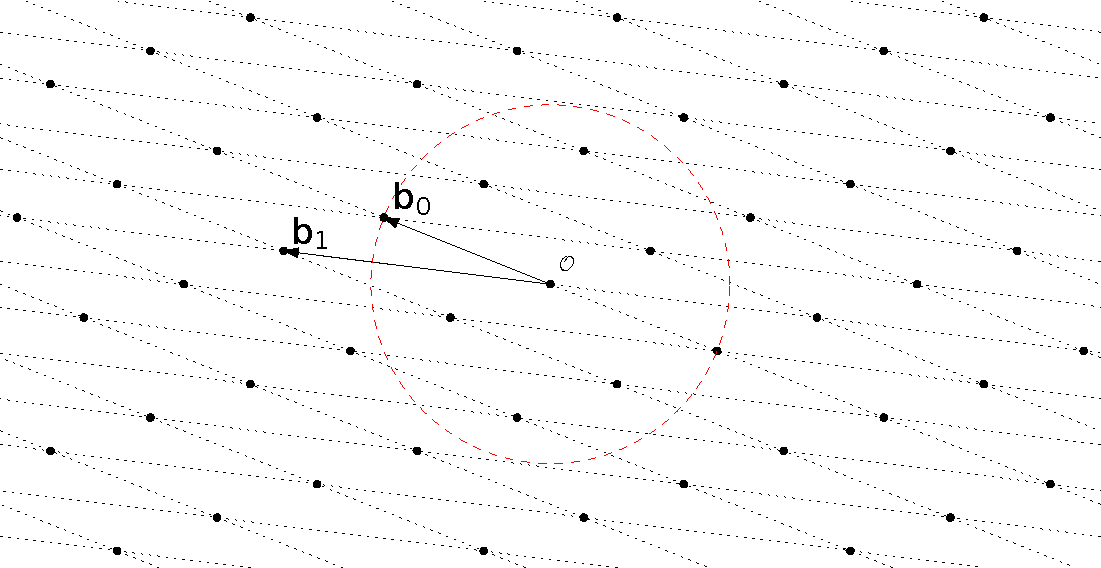
\includegraphics[width=.9\linewidth]{./assets/lattice-enumeration-0-radius.pdf}
\end{center}

\tiny Picture credit: Joop van de Pol
\end{frame}

\begin{frame}[label={sec:orgc957eaa}]{Enumeration II -- Project basis}
\begin{center}
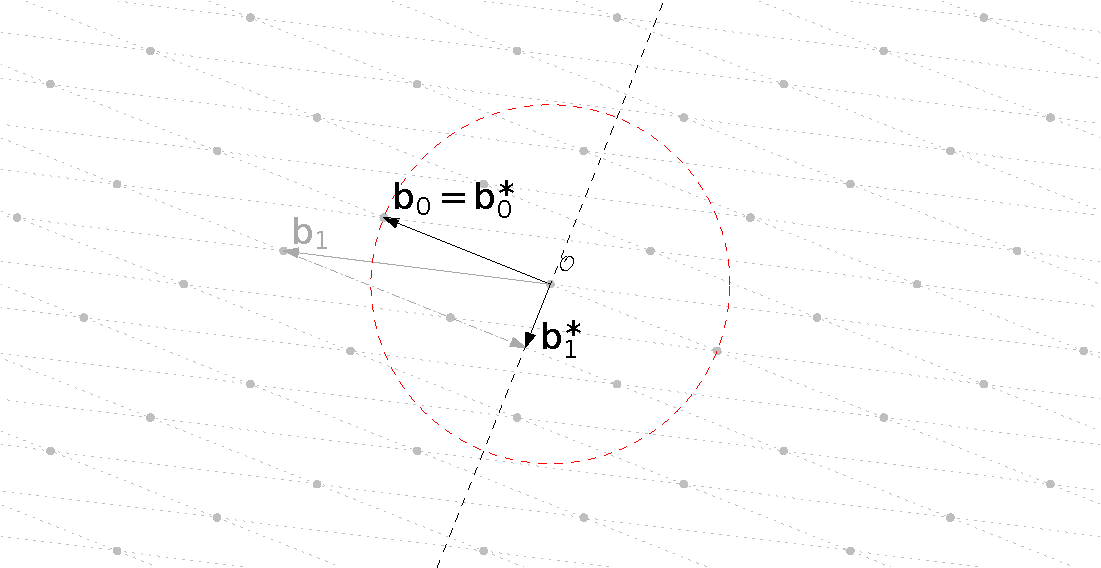
\includegraphics[width=.9\linewidth]{./assets/lattice-enumeration-1-project.pdf}
\end{center}

\tiny Picture credit: Joop van de Pol
\end{frame}

\begin{frame}[label={sec:org517ca73}]{Enumeration III -- Project lattice}
\begin{center}
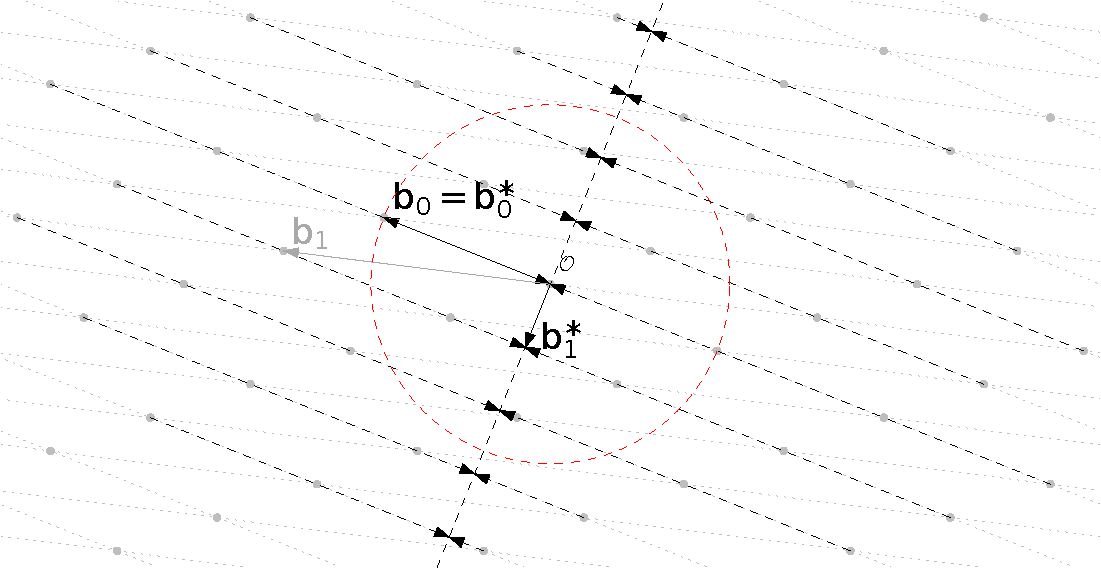
\includegraphics[width=.9\linewidth]{./assets/lattice-enumeration-2-project.pdf}
\end{center}

\tiny Picture credit: Joop van de Pol
\end{frame}

\begin{frame}[label={sec:org4ea77dc}]{Enumeration IV -- Enumerate projections}
\begin{center}
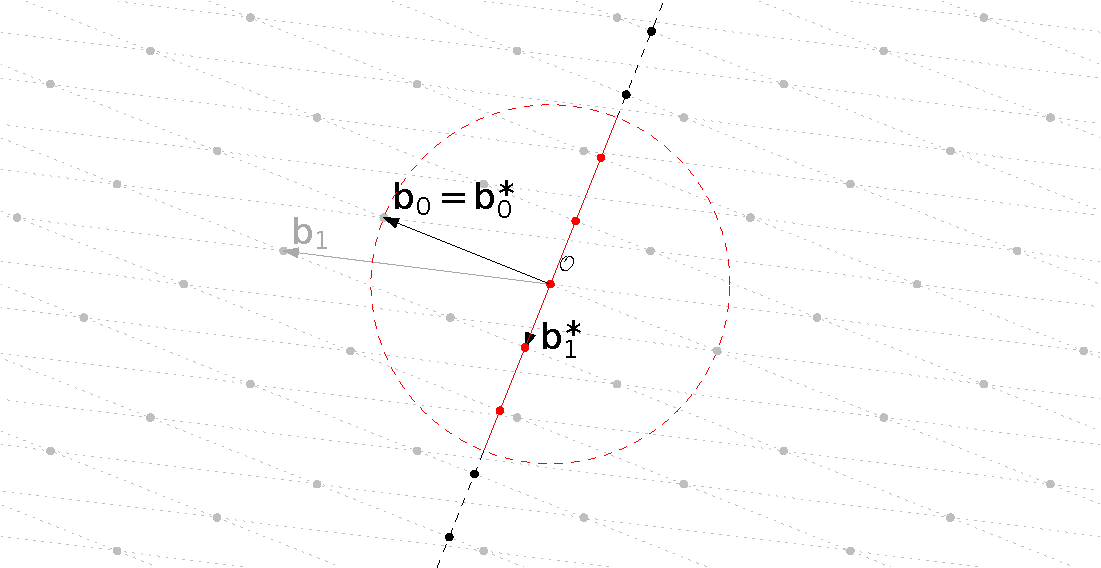
\includegraphics[width=.9\linewidth]{./assets/lattice-enumeration-3-enumerate.pdf}
\end{center}

\tiny Picture credit: Joop van de Pol
\end{frame}

\begin{frame}[label={sec:org495180f}]{Enumeration V -- For each lift and enumerate}
\begin{center}
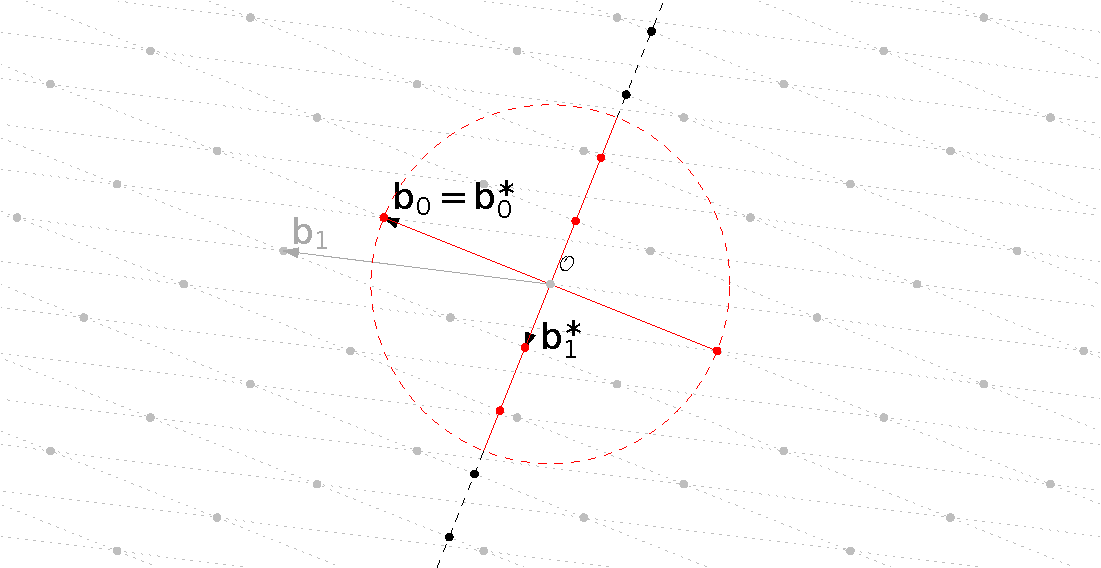
\includegraphics[width=.9\linewidth]{./assets/lattice-enumeration-4-lift.pdf}
\end{center}

\tiny Picture credit: Joop van de Pol
\end{frame}

\begin{frame}[label={sec:org894b9ef}]{Enumeration V -- For each lift and enumerate}
\begin{center}
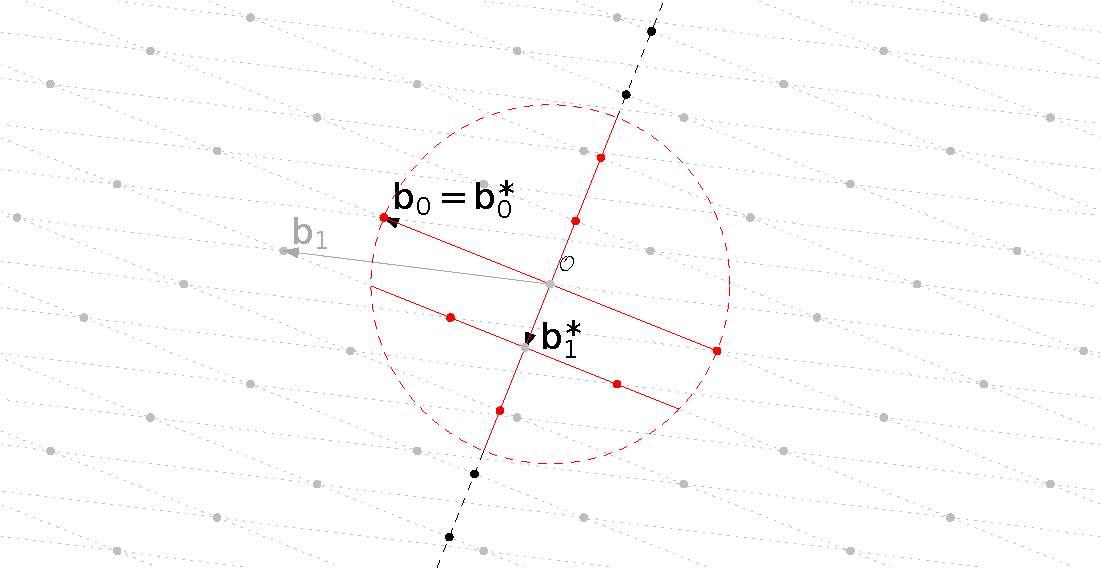
\includegraphics[width=.9\linewidth]{./assets/lattice-enumeration-5-lift.pdf}
\end{center}

\tiny Picture credit: Joop van de Pol
\end{frame}

\begin{frame}[label={sec:org44ed541}]{Enumeration VI -- Keep shortest}
\begin{center}
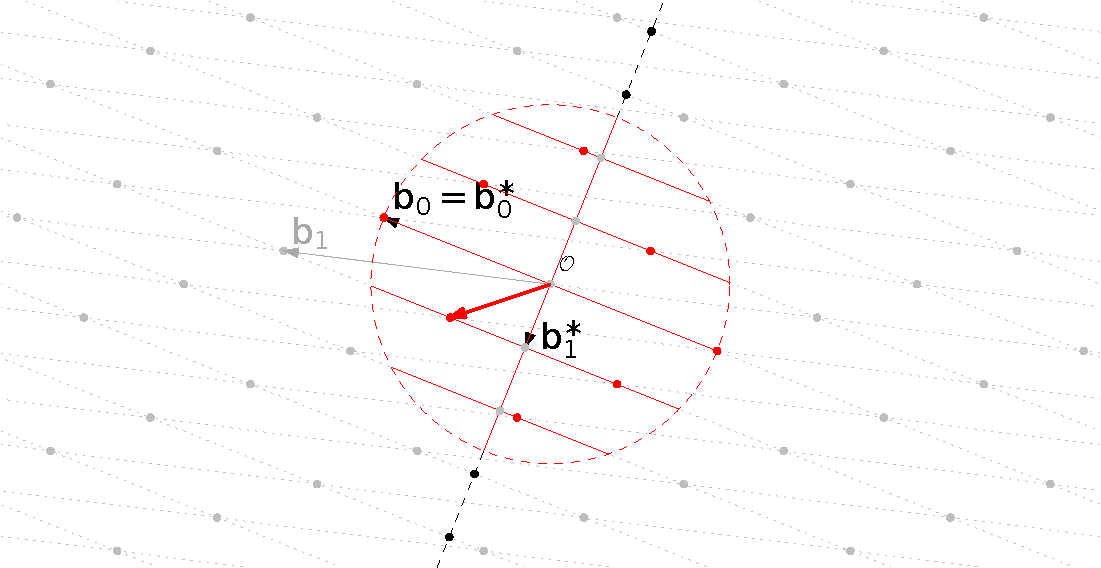
\includegraphics[width=.9\linewidth]{./assets/lattice-enumeration-6-keep.pdf}
\end{center}

\tiny Picture credit: Joop van de Pol
\end{frame}

\begin{frame}[label={sec:orga167370}]{Fast Enumeration}
\begin{itemize}
\item Do not exhaust the search space, but focus on a fraction with exponentially small probability of success, repeat exponentially often: speed-up \(2^{\Theta(\beta)}\)
\item Preprocess the basis with BKZ-\(\beta'\) for some \(\beta' \leq \beta\) before enumerating.
\end{itemize}
\end{frame}

\begin{frame}[label={sec:orga157c85}]{Enumeration Cost: \(\beta^{\beta/(2e) + o(\beta)}\)}
\tikzset{external/export=true}
\tikzsetnextfilename{enumeration-cost-2e}
\begin{tikzpicture}
  \begin{axis}[xmin=100,height=0.4\textwidth]
    \addplot table [x=d, col sep=comma, y expr = log2(\thisrowno{2})]%
    {data/fplll-simulations-enumeration-cost-2e.csv};
    \addlegendentry{FP(y)LLL simulation};
    \addplot+ [domain=100:500, samples=250]{0.1839*x*log2(x) - 0.995*x + 16.25};
    \addlegendentry{\(1/(2e)\, \beta \log(\beta) - 0.995\cdot \beta + 16.25\)};
  \end{axis}
\end{tikzpicture}
\tikzset{external/export=false}

\footnotesize \fullcite{C:ABFKSW20}
\end{frame}

\begin{frame}[label={sec:orgbce8a55}]{Enumeration Cost: \(\beta^{\beta/8 + o(\beta)}\)}
\begin{quote}
“Some authors favor the hypothesis that the average behaviour of an HKZ-reduced basis is rather a geometric decrease of the \(\|\vec{b}_i^{*}\|\)’s, i.e., roughly \(\|\vec{b}^*_i\| ≈ d^{\frac{i}{d}} \cdot \|\vec{b}_1\|\). With such a basis, solving SVP by Kannan’s algorithm would have a \(2^{O(d)} \cdot d^{\frac{d}{8}}\) complexity.”\footnote{Full version of \fullcite{C:HanSte07}, available at \url{http://perso.ens-lyon.fr/damien.stehle/KANNAN\_EXTENDED.html}}
\end{quote}
\end{frame}

\begin{frame}[label={sec:org710d922}]{\(1/8 = 0.125\) v \(1/(2e) \approx 0.184\)}
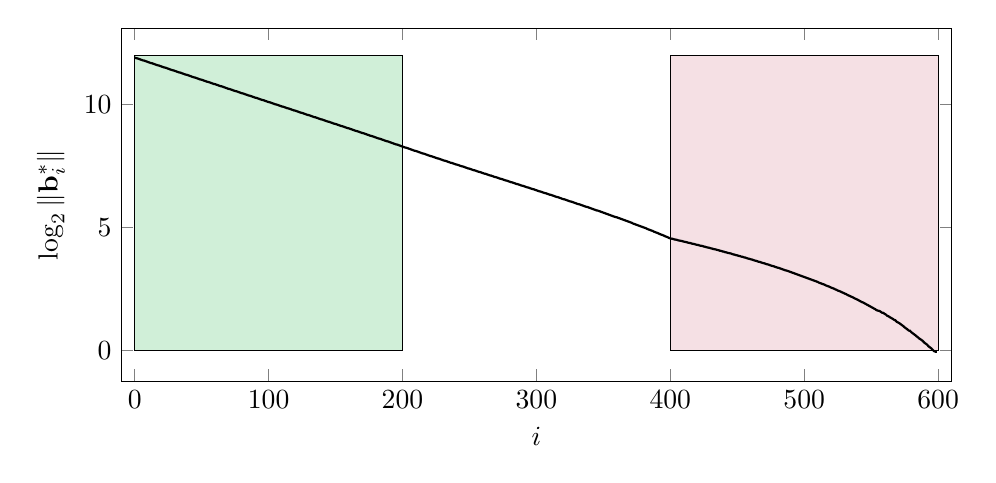
\begin{tikzpicture}
  \begin{axis}[xmin=-10, xmax=610, xlabel=\(i\),ylabel=\(\log_2 \|\vec{b}_i^*\|\),height=0.5\textwidth]
    \draw[fill=LightGreen!20!white,line width=0] (axis cs: 0,0) rectangle (axis cs: 200,12);
    \draw[fill=LightRed!20!white,line width=0] (axis cs: 400,0) rectangle (axis cs: 600,12);
    \addplot+[black] coordinates {
      (  0, 11.91) (  1, 11.89) (  2, 11.88) (  3, 11.86) (  4, 11.84) (  5, 11.82) (  6, 11.80)
      (  7, 11.79) (  8, 11.77) (  9, 11.75) ( 10, 11.73) ( 11, 11.71) ( 12, 11.69) ( 13, 11.68)
      ( 14, 11.66) ( 15, 11.64) ( 16, 11.62) ( 17, 11.60) ( 18, 11.59) ( 19, 11.57) ( 20, 11.55)
      ( 21, 11.53) ( 22, 11.51) ( 23, 11.50) ( 24, 11.48) ( 25, 11.46) ( 26, 11.44) ( 27, 11.42)
      ( 28, 11.40) ( 29, 11.39) ( 30, 11.37) ( 31, 11.35) ( 32, 11.33) ( 33, 11.31) ( 34, 11.30)
      ( 35, 11.28) ( 36, 11.26) ( 37, 11.24) ( 38, 11.22) ( 39, 11.21) ( 40, 11.19) ( 41, 11.17)
      ( 42, 11.15) ( 43, 11.13) ( 44, 11.11) ( 45, 11.10) ( 46, 11.08) ( 47, 11.06) ( 48, 11.04)
      ( 49, 11.02) ( 50, 11.01) ( 51, 10.99) ( 52, 10.97) ( 53, 10.95) ( 54, 10.93) ( 55, 10.92)
      ( 56, 10.90) ( 57, 10.88) ( 58, 10.86) ( 59, 10.84) ( 60, 10.83) ( 61, 10.81) ( 62, 10.79)
      ( 63, 10.77) ( 64, 10.75) ( 65, 10.74) ( 66, 10.72) ( 67, 10.70) ( 68, 10.68) ( 69, 10.66)
      ( 70, 10.64) ( 71, 10.63) ( 72, 10.61) ( 73, 10.59) ( 74, 10.57) ( 75, 10.55) ( 76, 10.54)
      ( 77, 10.52) ( 78, 10.50) ( 79, 10.48) ( 80, 10.46) ( 81, 10.45) ( 82, 10.43) ( 83, 10.41)
      ( 84, 10.39) ( 85, 10.37) ( 86, 10.36) ( 87, 10.34) ( 88, 10.32) ( 89, 10.30) ( 90, 10.28)
      ( 91, 10.27) ( 92, 10.25) ( 93, 10.23) ( 94, 10.21) ( 95, 10.19) ( 96, 10.18) ( 97, 10.16)
      ( 98, 10.14) ( 99, 10.12) (100, 10.10) (101, 10.09) (102, 10.07) (103, 10.05) (104, 10.03)
      (105, 10.01) (106, 10.00) (107,  9.98) (108,  9.96) (109,  9.94) (110,  9.92) (111,  9.91)
      (112,  9.89) (113,  9.87) (114,  9.85) (115,  9.84) (116,  9.82) (117,  9.80) (118,  9.78)
      (119,  9.76) (120,  9.75) (121,  9.73) (122,  9.71) (123,  9.69) (124,  9.67) (125,  9.66)
      (126,  9.64) (127,  9.62) (128,  9.60) (129,  9.58) (130,  9.57) (131,  9.55) (132,  9.53)
      (133,  9.51) (134,  9.49) (135,  9.48) (136,  9.46) (137,  9.44) (138,  9.42) (139,  9.40)
      (140,  9.39) (141,  9.37) (142,  9.35) (143,  9.33) (144,  9.31) (145,  9.30) (146,  9.28)
      (147,  9.26) (148,  9.24) (149,  9.22) (150,  9.21) (151,  9.19) (152,  9.17) (153,  9.15)
      (154,  9.13) (155,  9.12) (156,  9.10) (157,  9.08) (158,  9.06) (159,  9.04) (160,  9.03)
      (161,  9.01) (162,  8.99) (163,  8.97) (164,  8.95) (165,  8.93) (166,  8.92) (167,  8.90)
      (168,  8.88) (169,  8.86) (170,  8.84) (171,  8.83) (172,  8.81) (173,  8.79) (174,  8.77)
      (175,  8.75) (176,  8.73) (177,  8.72) (178,  8.70) (179,  8.68) (180,  8.66) (181,  8.64)
      (182,  8.62) (183,  8.61) (184,  8.59) (185,  8.57) (186,  8.55) (187,  8.53) (188,  8.51)
      (189,  8.50) (190,  8.48) (191,  8.46) (192,  8.44) (193,  8.42) (194,  8.40) (195,  8.38)
      (196,  8.37) (197,  8.35) (198,  8.33) (199,  8.31) (200,  8.29) (201,  8.27) (202,  8.25)
      (203,  8.24) (204,  8.22) (205,  8.20) (206,  8.18) (207,  8.16) (208,  8.14) (209,  8.12)
      (210,  8.11) (211,  8.09) (212,  8.07) (213,  8.05) (214,  8.03) (215,  8.01) (216,  8.00)
      (217,  7.98) (218,  7.96) (219,  7.94) (220,  7.92) (221,  7.90) (222,  7.89) (223,  7.87)
      (224,  7.85) (225,  7.83) (226,  7.81) (227,  7.80) (228,  7.78) (229,  7.76) (230,  7.74)
      (231,  7.72) (232,  7.71) (233,  7.69) (234,  7.67) (235,  7.65) (236,  7.63) (237,  7.62)
      (238,  7.60) (239,  7.58) (240,  7.56) (241,  7.55) (242,  7.53) (243,  7.51) (244,  7.49)
      (245,  7.48) (246,  7.46) (247,  7.44) (248,  7.42) (249,  7.40) (250,  7.39) (251,  7.37)
      (252,  7.35) (253,  7.33) (254,  7.32) (255,  7.30) (256,  7.28) (257,  7.26) (258,  7.25)
      (259,  7.23) (260,  7.21) (261,  7.19) (262,  7.18) (263,  7.16) (264,  7.14) (265,  7.12)
      (266,  7.11) (267,  7.09) (268,  7.07) (269,  7.05) (270,  7.04) (271,  7.02) (272,  7.00)
      (273,  6.98) (274,  6.97) (275,  6.95) (276,  6.93) (277,  6.91) (278,  6.90) (279,  6.88)
      (280,  6.86) (281,  6.84) (282,  6.83) (283,  6.81) (284,  6.79) (285,  6.77) (286,  6.76)
      (287,  6.74) (288,  6.72) (289,  6.70) (290,  6.69) (291,  6.67) (292,  6.65) (293,  6.63)
      (294,  6.62) (295,  6.60) (296,  6.58) (297,  6.56) (298,  6.55) (299,  6.53) (300,  6.51)
      (301,  6.49) (302,  6.47) (303,  6.46) (304,  6.44) (305,  6.42) (306,  6.40) (307,  6.39)
      (308,  6.37) (309,  6.35) (310,  6.33) (311,  6.32) (312,  6.30) (313,  6.28) (314,  6.26)
      (315,  6.24) (316,  6.23) (317,  6.21) (318,  6.19) (319,  6.17) (320,  6.15) (321,  6.14)
      (322,  6.12) (323,  6.10) (324,  6.08) (325,  6.06) (326,  6.05) (327,  6.03) (328,  6.01)
      (329,  5.99) (330,  5.97) (331,  5.95) (332,  5.94) (333,  5.92) (334,  5.90) (335,  5.88)
      (336,  5.86) (337,  5.84) (338,  5.83) (339,  5.81) (340,  5.79) (341,  5.77) (342,  5.75)
      (343,  5.73) (344,  5.71) (345,  5.69) (346,  5.68) (347,  5.66) (348,  5.64) (349,  5.62)
      (350,  5.60) (351,  5.58) (352,  5.56) (353,  5.54) (354,  5.52) (355,  5.50) (356,  5.48)
      (357,  5.46) (358,  5.44) (359,  5.42) (360,  5.41) (361,  5.39) (362,  5.37) (363,  5.35)
      (364,  5.33) (365,  5.31) (366,  5.29) (367,  5.27) (368,  5.25) (369,  5.23) (370,  5.21)
      (371,  5.19) (372,  5.16) (373,  5.14) (374,  5.12) (375,  5.10) (376,  5.08) (377,  5.06)
      (378,  5.04) (379,  5.02) (380,  5.00) (381,  4.98) (382,  4.96) (383,  4.93) (384,  4.91)
      (385,  4.89) (386,  4.87) (387,  4.85) (388,  4.82) (389,  4.80) (390,  4.78) (391,  4.76)
      (392,  4.73) (393,  4.71) (394,  4.69) (395,  4.67) (396,  4.64) (397,  4.62) (398,  4.60)
      (399,  4.57) (400,  4.55) (401,  4.54) (402,  4.53) (403,  4.51) (404,  4.50) (405,  4.49)
      (406,  4.47) (407,  4.46) (408,  4.45) (409,  4.44) (410,  4.42) (411,  4.41) (412,  4.40)
      (413,  4.38) (414,  4.37) (415,  4.36) (416,  4.34) (417,  4.33) (418,  4.32) (419,  4.30)
      (420,  4.29) (421,  4.28) (422,  4.26) (423,  4.25) (424,  4.24) (425,  4.22) (426,  4.21)
      (427,  4.19) (428,  4.18) (429,  4.17) (430,  4.15) (431,  4.14) (432,  4.12) (433,  4.11)
      (434,  4.10) (435,  4.08) (436,  4.07) (437,  4.05) (438,  4.04) (439,  4.02) (440,  4.01)
      (441,  3.99) (442,  3.98) (443,  3.96) (444,  3.95) (445,  3.94) (446,  3.92) (447,  3.90)
      (448,  3.89) (449,  3.87) (450,  3.86) (451,  3.84) (452,  3.83) (453,  3.81) (454,  3.80)
      (455,  3.78) (456,  3.77) (457,  3.75) (458,  3.73) (459,  3.72) (460,  3.70) (461,  3.69)
      (462,  3.67) (463,  3.65) (464,  3.64) (465,  3.62) (466,  3.60) (467,  3.59) (468,  3.57)
      (469,  3.55) (470,  3.54) (471,  3.52) (472,  3.50) (473,  3.49) (474,  3.47) (475,  3.45)
      (476,  3.43) (477,  3.42) (478,  3.40) (479,  3.38) (480,  3.36) (481,  3.35) (482,  3.33)
      (483,  3.31) (484,  3.29) (485,  3.27) (486,  3.25) (487,  3.24) (488,  3.22) (489,  3.20)
      (490,  3.18) (491,  3.16) (492,  3.14) (493,  3.12) (494,  3.10) (495,  3.08) (496,  3.06)
      (497,  3.04) (498,  3.02) (499,  3.00) (500,  2.98) (501,  2.96) (502,  2.94) (503,  2.92)
      (504,  2.90) (505,  2.88) (506,  2.86) (507,  2.84) (508,  2.82) (509,  2.80) (510,  2.78)
      (511,  2.75) (512,  2.73) (513,  2.71) (514,  2.69) (515,  2.67) (516,  2.64) (517,  2.62)
      (518,  2.60) (519,  2.58) (520,  2.55) (521,  2.53) (522,  2.51) (523,  2.48) (524,  2.46)
      (525,  2.43) (526,  2.41) (527,  2.39) (528,  2.36) (529,  2.34) (530,  2.31) (531,  2.29)
      (532,  2.26) (533,  2.23) (534,  2.21) (535,  2.18) (536,  2.16) (537,  2.13) (538,  2.10)
      (539,  2.08) (540,  2.05) (541,  2.02) (542,  1.99) (543,  1.96) (544,  1.94) (545,  1.91)
      (546,  1.88) (547,  1.85) (548,  1.82) (549,  1.79) (550,  1.76) (551,  1.73) (552,  1.70)
      (553,  1.67) (554,  1.63) (555,  1.61) (556,  1.60) (557,  1.57) (558,  1.53) (559,  1.52)
      (560,  1.48) (561,  1.45) (562,  1.40) (563,  1.38) (564,  1.34) (565,  1.31) (566,  1.28)
      (567,  1.24) (568,  1.22) (569,  1.16) (570,  1.13) (571,  1.10) (572,  1.06) (573,  1.02)
      (574,  0.98) (575,  0.93) (576,  0.89) (577,  0.85) (578,  0.80) (579,  0.79) (580,  0.73)
      (581,  0.69) (582,  0.65) (583,  0.61) (584,  0.56) (585,  0.52) (586,  0.47) (587,  0.44)
      (588,  0.40) (589,  0.35) (590,  0.29) (591,  0.26) (592,  0.21) (593,  0.15) (594,  0.11)
      (595,  0.07) (596,  0.01) (597, -0.04) (598, -0.06) (599, -0.06) 
    };
  \end{axis}
\end{tikzpicture}
\end{frame}

\begin{frame}[label={sec:orgb88c94a}]{Why we can’t have Nice Things™}
\begin{enumerate}
\item We run enumeration many times each succeeding with low probability of success and re-randomise in between: this destroys the nice GSA-line shape
\begin{itemize}
\item Thus, before enumerating a local block, we run some local preprocessing with some block size \(\beta' < \beta\)
\end{itemize}
\item In the sandpile model,\footfullcite{C:HanPujSte11} as the algorithm proceeds through the indices \(i\), a “bump” accumulates from index \(i + 1\) onward.
\end{enumerate}
\end{frame}

\begin{frame}[label={sec:org1d4d0c1}]{Idea: Overshoot Preprocessing}
\tikzset{external/export=true}
\tikzsetnextfilename{enumeration-cost-overshooting-idea}
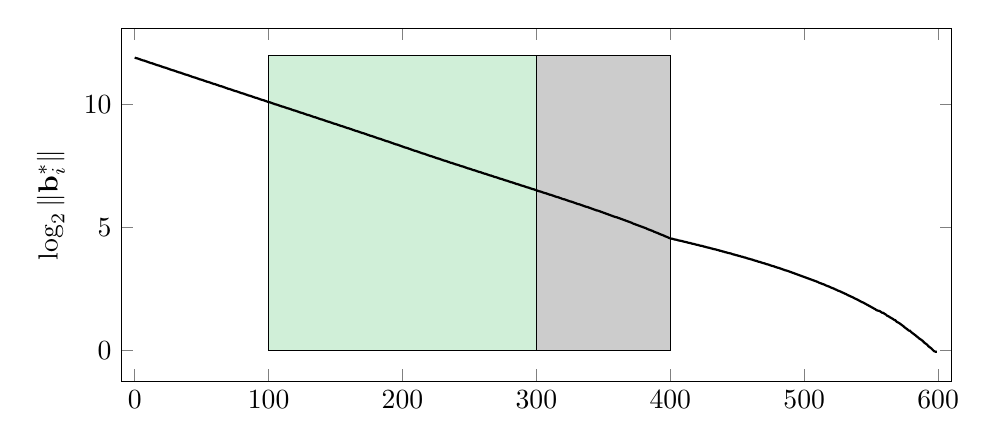
\begin{tikzpicture}
  \begin{axis}[xmin=-10, xmax=610, xlabel=,ylabel=\(\log_2 \|\vec{b}_i^*\|\),height=0.5\textwidth]
    \draw[fill=black!20!white,line width=0] (axis cs: 100,0) rectangle (axis cs: 400,12);
    \draw[fill=LightGreen!20!white,line width=0] (axis cs: 100,0) rectangle (axis cs: 300,12);
    \addplot+[black] coordinates {
      (  0, 11.91) (  1, 11.89) (  2, 11.88) (  3, 11.86) (  4, 11.84) (  5, 11.82) (  6, 11.80)
      (  7, 11.79) (  8, 11.77) (  9, 11.75) ( 10, 11.73) ( 11, 11.71) ( 12, 11.69) ( 13, 11.68)
      ( 14, 11.66) ( 15, 11.64) ( 16, 11.62) ( 17, 11.60) ( 18, 11.59) ( 19, 11.57) ( 20, 11.55)
      ( 21, 11.53) ( 22, 11.51) ( 23, 11.50) ( 24, 11.48) ( 25, 11.46) ( 26, 11.44) ( 27, 11.42)
      ( 28, 11.40) ( 29, 11.39) ( 30, 11.37) ( 31, 11.35) ( 32, 11.33) ( 33, 11.31) ( 34, 11.30)
      ( 35, 11.28) ( 36, 11.26) ( 37, 11.24) ( 38, 11.22) ( 39, 11.21) ( 40, 11.19) ( 41, 11.17)
      ( 42, 11.15) ( 43, 11.13) ( 44, 11.11) ( 45, 11.10) ( 46, 11.08) ( 47, 11.06) ( 48, 11.04)
      ( 49, 11.02) ( 50, 11.01) ( 51, 10.99) ( 52, 10.97) ( 53, 10.95) ( 54, 10.93) ( 55, 10.92)
      ( 56, 10.90) ( 57, 10.88) ( 58, 10.86) ( 59, 10.84) ( 60, 10.83) ( 61, 10.81) ( 62, 10.79)
      ( 63, 10.77) ( 64, 10.75) ( 65, 10.74) ( 66, 10.72) ( 67, 10.70) ( 68, 10.68) ( 69, 10.66)
      ( 70, 10.64) ( 71, 10.63) ( 72, 10.61) ( 73, 10.59) ( 74, 10.57) ( 75, 10.55) ( 76, 10.54)
      ( 77, 10.52) ( 78, 10.50) ( 79, 10.48) ( 80, 10.46) ( 81, 10.45) ( 82, 10.43) ( 83, 10.41)
      ( 84, 10.39) ( 85, 10.37) ( 86, 10.36) ( 87, 10.34) ( 88, 10.32) ( 89, 10.30) ( 90, 10.28)
      ( 91, 10.27) ( 92, 10.25) ( 93, 10.23) ( 94, 10.21) ( 95, 10.19) ( 96, 10.18) ( 97, 10.16)
      ( 98, 10.14) ( 99, 10.12) (100, 10.10) (101, 10.09) (102, 10.07) (103, 10.05) (104, 10.03)
      (105, 10.01) (106, 10.00) (107,  9.98) (108,  9.96) (109,  9.94) (110,  9.92) (111,  9.91)
      (112,  9.89) (113,  9.87) (114,  9.85) (115,  9.84) (116,  9.82) (117,  9.80) (118,  9.78)
      (119,  9.76) (120,  9.75) (121,  9.73) (122,  9.71) (123,  9.69) (124,  9.67) (125,  9.66)
      (126,  9.64) (127,  9.62) (128,  9.60) (129,  9.58) (130,  9.57) (131,  9.55) (132,  9.53)
      (133,  9.51) (134,  9.49) (135,  9.48) (136,  9.46) (137,  9.44) (138,  9.42) (139,  9.40)
      (140,  9.39) (141,  9.37) (142,  9.35) (143,  9.33) (144,  9.31) (145,  9.30) (146,  9.28)
      (147,  9.26) (148,  9.24) (149,  9.22) (150,  9.21) (151,  9.19) (152,  9.17) (153,  9.15)
      (154,  9.13) (155,  9.12) (156,  9.10) (157,  9.08) (158,  9.06) (159,  9.04) (160,  9.03)
      (161,  9.01) (162,  8.99) (163,  8.97) (164,  8.95) (165,  8.93) (166,  8.92) (167,  8.90)
      (168,  8.88) (169,  8.86) (170,  8.84) (171,  8.83) (172,  8.81) (173,  8.79) (174,  8.77)
      (175,  8.75) (176,  8.73) (177,  8.72) (178,  8.70) (179,  8.68) (180,  8.66) (181,  8.64)
      (182,  8.62) (183,  8.61) (184,  8.59) (185,  8.57) (186,  8.55) (187,  8.53) (188,  8.51)
      (189,  8.50) (190,  8.48) (191,  8.46) (192,  8.44) (193,  8.42) (194,  8.40) (195,  8.38)
      (196,  8.37) (197,  8.35) (198,  8.33) (199,  8.31) (200,  8.29) (201,  8.27) (202,  8.25)
      (203,  8.24) (204,  8.22) (205,  8.20) (206,  8.18) (207,  8.16) (208,  8.14) (209,  8.12)
      (210,  8.11) (211,  8.09) (212,  8.07) (213,  8.05) (214,  8.03) (215,  8.01) (216,  8.00)
      (217,  7.98) (218,  7.96) (219,  7.94) (220,  7.92) (221,  7.90) (222,  7.89) (223,  7.87)
      (224,  7.85) (225,  7.83) (226,  7.81) (227,  7.80) (228,  7.78) (229,  7.76) (230,  7.74)
      (231,  7.72) (232,  7.71) (233,  7.69) (234,  7.67) (235,  7.65) (236,  7.63) (237,  7.62)
      (238,  7.60) (239,  7.58) (240,  7.56) (241,  7.55) (242,  7.53) (243,  7.51) (244,  7.49)
      (245,  7.48) (246,  7.46) (247,  7.44) (248,  7.42) (249,  7.40) (250,  7.39) (251,  7.37)
      (252,  7.35) (253,  7.33) (254,  7.32) (255,  7.30) (256,  7.28) (257,  7.26) (258,  7.25)
      (259,  7.23) (260,  7.21) (261,  7.19) (262,  7.18) (263,  7.16) (264,  7.14) (265,  7.12)
      (266,  7.11) (267,  7.09) (268,  7.07) (269,  7.05) (270,  7.04) (271,  7.02) (272,  7.00)
      (273,  6.98) (274,  6.97) (275,  6.95) (276,  6.93) (277,  6.91) (278,  6.90) (279,  6.88)
      (280,  6.86) (281,  6.84) (282,  6.83) (283,  6.81) (284,  6.79) (285,  6.77) (286,  6.76)
      (287,  6.74) (288,  6.72) (289,  6.70) (290,  6.69) (291,  6.67) (292,  6.65) (293,  6.63)
      (294,  6.62) (295,  6.60) (296,  6.58) (297,  6.56) (298,  6.55) (299,  6.53) (300,  6.51)
      (301,  6.49) (302,  6.47) (303,  6.46) (304,  6.44) (305,  6.42) (306,  6.40) (307,  6.39)
      (308,  6.37) (309,  6.35) (310,  6.33) (311,  6.32) (312,  6.30) (313,  6.28) (314,  6.26)
      (315,  6.24) (316,  6.23) (317,  6.21) (318,  6.19) (319,  6.17) (320,  6.15) (321,  6.14)
      (322,  6.12) (323,  6.10) (324,  6.08) (325,  6.06) (326,  6.05) (327,  6.03) (328,  6.01)
      (329,  5.99) (330,  5.97) (331,  5.95) (332,  5.94) (333,  5.92) (334,  5.90) (335,  5.88)
      (336,  5.86) (337,  5.84) (338,  5.83) (339,  5.81) (340,  5.79) (341,  5.77) (342,  5.75)
      (343,  5.73) (344,  5.71) (345,  5.69) (346,  5.68) (347,  5.66) (348,  5.64) (349,  5.62)
      (350,  5.60) (351,  5.58) (352,  5.56) (353,  5.54) (354,  5.52) (355,  5.50) (356,  5.48)
      (357,  5.46) (358,  5.44) (359,  5.42) (360,  5.41) (361,  5.39) (362,  5.37) (363,  5.35)
      (364,  5.33) (365,  5.31) (366,  5.29) (367,  5.27) (368,  5.25) (369,  5.23) (370,  5.21)
      (371,  5.19) (372,  5.16) (373,  5.14) (374,  5.12) (375,  5.10) (376,  5.08) (377,  5.06)
      (378,  5.04) (379,  5.02) (380,  5.00) (381,  4.98) (382,  4.96) (383,  4.93) (384,  4.91)
      (385,  4.89) (386,  4.87) (387,  4.85) (388,  4.82) (389,  4.80) (390,  4.78) (391,  4.76)
      (392,  4.73) (393,  4.71) (394,  4.69) (395,  4.67) (396,  4.64) (397,  4.62) (398,  4.60)
      (399,  4.57) (400,  4.55) (401,  4.54) (402,  4.53) (403,  4.51) (404,  4.50) (405,  4.49)
      (406,  4.47) (407,  4.46) (408,  4.45) (409,  4.44) (410,  4.42) (411,  4.41) (412,  4.40)
      (413,  4.38) (414,  4.37) (415,  4.36) (416,  4.34) (417,  4.33) (418,  4.32) (419,  4.30)
      (420,  4.29) (421,  4.28) (422,  4.26) (423,  4.25) (424,  4.24) (425,  4.22) (426,  4.21)
      (427,  4.19) (428,  4.18) (429,  4.17) (430,  4.15) (431,  4.14) (432,  4.12) (433,  4.11)
      (434,  4.10) (435,  4.08) (436,  4.07) (437,  4.05) (438,  4.04) (439,  4.02) (440,  4.01)
      (441,  3.99) (442,  3.98) (443,  3.96) (444,  3.95) (445,  3.94) (446,  3.92) (447,  3.90)
      (448,  3.89) (449,  3.87) (450,  3.86) (451,  3.84) (452,  3.83) (453,  3.81) (454,  3.80)
      (455,  3.78) (456,  3.77) (457,  3.75) (458,  3.73) (459,  3.72) (460,  3.70) (461,  3.69)
      (462,  3.67) (463,  3.65) (464,  3.64) (465,  3.62) (466,  3.60) (467,  3.59) (468,  3.57)
      (469,  3.55) (470,  3.54) (471,  3.52) (472,  3.50) (473,  3.49) (474,  3.47) (475,  3.45)
      (476,  3.43) (477,  3.42) (478,  3.40) (479,  3.38) (480,  3.36) (481,  3.35) (482,  3.33)
      (483,  3.31) (484,  3.29) (485,  3.27) (486,  3.25) (487,  3.24) (488,  3.22) (489,  3.20)
      (490,  3.18) (491,  3.16) (492,  3.14) (493,  3.12) (494,  3.10) (495,  3.08) (496,  3.06)
      (497,  3.04) (498,  3.02) (499,  3.00) (500,  2.98) (501,  2.96) (502,  2.94) (503,  2.92)
      (504,  2.90) (505,  2.88) (506,  2.86) (507,  2.84) (508,  2.82) (509,  2.80) (510,  2.78)
      (511,  2.75) (512,  2.73) (513,  2.71) (514,  2.69) (515,  2.67) (516,  2.64) (517,  2.62)
      (518,  2.60) (519,  2.58) (520,  2.55) (521,  2.53) (522,  2.51) (523,  2.48) (524,  2.46)
      (525,  2.43) (526,  2.41) (527,  2.39) (528,  2.36) (529,  2.34) (530,  2.31) (531,  2.29)
      (532,  2.26) (533,  2.23) (534,  2.21) (535,  2.18) (536,  2.16) (537,  2.13) (538,  2.10)
      (539,  2.08) (540,  2.05) (541,  2.02) (542,  1.99) (543,  1.96) (544,  1.94) (545,  1.91)
      (546,  1.88) (547,  1.85) (548,  1.82) (549,  1.79) (550,  1.76) (551,  1.73) (552,  1.70)
      (553,  1.67) (554,  1.63) (555,  1.61) (556,  1.60) (557,  1.57) (558,  1.53) (559,  1.52)
      (560,  1.48) (561,  1.45) (562,  1.40) (563,  1.38) (564,  1.34) (565,  1.31) (566,  1.28)
      (567,  1.24) (568,  1.22) (569,  1.16) (570,  1.13) (571,  1.10) (572,  1.06) (573,  1.02)
      (574,  0.98) (575,  0.93) (576,  0.89) (577,  0.85) (578,  0.80) (579,  0.79) (580,  0.73)
      (581,  0.69) (582,  0.65) (583,  0.61) (584,  0.56) (585,  0.52) (586,  0.47) (587,  0.44)
      (588,  0.40) (589,  0.35) (590,  0.29) (591,  0.26) (592,  0.21) (593,  0.15) (594,  0.11)
      (595,  0.07) (596,  0.01) (597, -0.04) (598, -0.06) (599, -0.06) 
    };
  \end{axis}
\end{tikzpicture}
\tikzset{external/export=false}

\begin{center}
Preprocessing in dimension \((1+c)\cdot \beta\) for enumeration in dimension \(\beta\).
\end{center}
\end{frame}

\begin{frame}[label={sec:org53921e2}]{Practical Performance (Simulation)}
\tikzset{external/export=true}
\tikzsetnextfilename{enumeration-cost-8}
\begin{tikzpicture}
  \begin{axis}[height=0.4\textwidth]
    \addplot+ [domain=100:500, samples=250]{0.1839*x*log2(x) - 0.995*x + 16.25};
    \addlegendentry{\(1/(2e)\, \beta \log(\beta) - 0.995\cdot \beta + 16.25\)};
    \addplot table [x=d, col sep=comma, y expr = log2(\thisrowno{2})]%
    {data/fplll-simulations-enumeration-cost-8-c=0.25.csv};
    \addlegendentry{simulation};
    \addplot+ [domain=20:500, samples=100]{0.125*x*log2(x) + -0.547*x + 10.4};
    \addlegendentry{\(1/8\,\beta\log(\beta) - 0.547\beta + 10.4\) for \(c=1/4\)}
  \end{axis}
\end{tikzpicture}
\tikzset{external/export=false}

\footnotesize \fullcite{C:ABFKSW20}
\end{frame}

\begin{frame}[label={sec:orgccac359}]{Open Question: Can we do better?}
\tikzset{external/export=true}
\tikzsetnextfilename{enumeration-cost-better-shape}
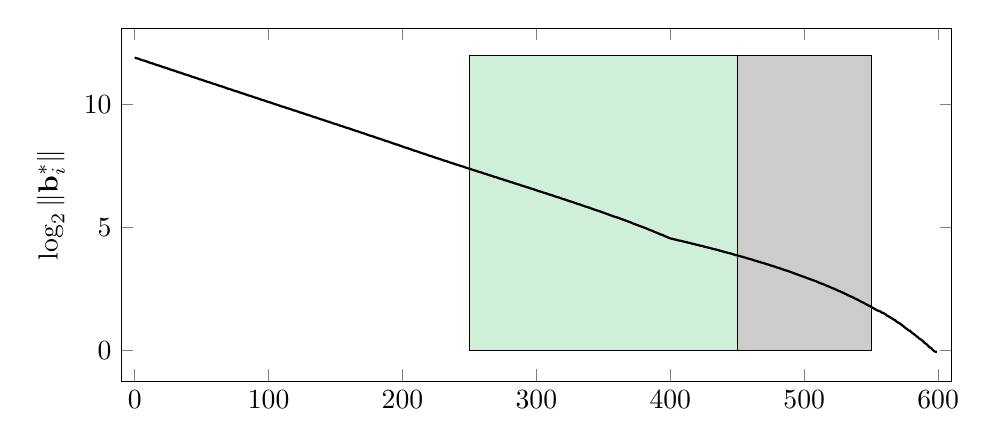
\begin{tikzpicture}
  \begin{axis}[xmin=-10, xmax=610, xlabel=,ylabel=\(\log_2 \|\vec{b}_i^*\|\),height=0.5\textwidth]
    \draw[fill=black!20!white,line width=0] (axis cs: 250,0) rectangle (axis cs: 550,12);
    \draw[fill=LightGreen!20!white,line width=0] (axis cs: 250,0) rectangle (axis cs: 450,12);
    \addplot+[black] coordinates {
      (  0, 11.91) (  1, 11.89) (  2, 11.88) (  3, 11.86) (  4, 11.84) (  5, 11.82) (  6, 11.80)
      (  7, 11.79) (  8, 11.77) (  9, 11.75) ( 10, 11.73) ( 11, 11.71) ( 12, 11.69) ( 13, 11.68)
      ( 14, 11.66) ( 15, 11.64) ( 16, 11.62) ( 17, 11.60) ( 18, 11.59) ( 19, 11.57) ( 20, 11.55)
      ( 21, 11.53) ( 22, 11.51) ( 23, 11.50) ( 24, 11.48) ( 25, 11.46) ( 26, 11.44) ( 27, 11.42)
      ( 28, 11.40) ( 29, 11.39) ( 30, 11.37) ( 31, 11.35) ( 32, 11.33) ( 33, 11.31) ( 34, 11.30)
      ( 35, 11.28) ( 36, 11.26) ( 37, 11.24) ( 38, 11.22) ( 39, 11.21) ( 40, 11.19) ( 41, 11.17)
      ( 42, 11.15) ( 43, 11.13) ( 44, 11.11) ( 45, 11.10) ( 46, 11.08) ( 47, 11.06) ( 48, 11.04)
      ( 49, 11.02) ( 50, 11.01) ( 51, 10.99) ( 52, 10.97) ( 53, 10.95) ( 54, 10.93) ( 55, 10.92)
      ( 56, 10.90) ( 57, 10.88) ( 58, 10.86) ( 59, 10.84) ( 60, 10.83) ( 61, 10.81) ( 62, 10.79)
      ( 63, 10.77) ( 64, 10.75) ( 65, 10.74) ( 66, 10.72) ( 67, 10.70) ( 68, 10.68) ( 69, 10.66)
      ( 70, 10.64) ( 71, 10.63) ( 72, 10.61) ( 73, 10.59) ( 74, 10.57) ( 75, 10.55) ( 76, 10.54)
      ( 77, 10.52) ( 78, 10.50) ( 79, 10.48) ( 80, 10.46) ( 81, 10.45) ( 82, 10.43) ( 83, 10.41)
      ( 84, 10.39) ( 85, 10.37) ( 86, 10.36) ( 87, 10.34) ( 88, 10.32) ( 89, 10.30) ( 90, 10.28)
      ( 91, 10.27) ( 92, 10.25) ( 93, 10.23) ( 94, 10.21) ( 95, 10.19) ( 96, 10.18) ( 97, 10.16)
      ( 98, 10.14) ( 99, 10.12) (100, 10.10) (101, 10.09) (102, 10.07) (103, 10.05) (104, 10.03)
      (105, 10.01) (106, 10.00) (107,  9.98) (108,  9.96) (109,  9.94) (110,  9.92) (111,  9.91)
      (112,  9.89) (113,  9.87) (114,  9.85) (115,  9.84) (116,  9.82) (117,  9.80) (118,  9.78)
      (119,  9.76) (120,  9.75) (121,  9.73) (122,  9.71) (123,  9.69) (124,  9.67) (125,  9.66)
      (126,  9.64) (127,  9.62) (128,  9.60) (129,  9.58) (130,  9.57) (131,  9.55) (132,  9.53)
      (133,  9.51) (134,  9.49) (135,  9.48) (136,  9.46) (137,  9.44) (138,  9.42) (139,  9.40)
      (140,  9.39) (141,  9.37) (142,  9.35) (143,  9.33) (144,  9.31) (145,  9.30) (146,  9.28)
      (147,  9.26) (148,  9.24) (149,  9.22) (150,  9.21) (151,  9.19) (152,  9.17) (153,  9.15)
      (154,  9.13) (155,  9.12) (156,  9.10) (157,  9.08) (158,  9.06) (159,  9.04) (160,  9.03)
      (161,  9.01) (162,  8.99) (163,  8.97) (164,  8.95) (165,  8.93) (166,  8.92) (167,  8.90)
      (168,  8.88) (169,  8.86) (170,  8.84) (171,  8.83) (172,  8.81) (173,  8.79) (174,  8.77)
      (175,  8.75) (176,  8.73) (177,  8.72) (178,  8.70) (179,  8.68) (180,  8.66) (181,  8.64)
      (182,  8.62) (183,  8.61) (184,  8.59) (185,  8.57) (186,  8.55) (187,  8.53) (188,  8.51)
      (189,  8.50) (190,  8.48) (191,  8.46) (192,  8.44) (193,  8.42) (194,  8.40) (195,  8.38)
      (196,  8.37) (197,  8.35) (198,  8.33) (199,  8.31) (200,  8.29) (201,  8.27) (202,  8.25)
      (203,  8.24) (204,  8.22) (205,  8.20) (206,  8.18) (207,  8.16) (208,  8.14) (209,  8.12)
      (210,  8.11) (211,  8.09) (212,  8.07) (213,  8.05) (214,  8.03) (215,  8.01) (216,  8.00)
      (217,  7.98) (218,  7.96) (219,  7.94) (220,  7.92) (221,  7.90) (222,  7.89) (223,  7.87)
      (224,  7.85) (225,  7.83) (226,  7.81) (227,  7.80) (228,  7.78) (229,  7.76) (230,  7.74)
      (231,  7.72) (232,  7.71) (233,  7.69) (234,  7.67) (235,  7.65) (236,  7.63) (237,  7.62)
      (238,  7.60) (239,  7.58) (240,  7.56) (241,  7.55) (242,  7.53) (243,  7.51) (244,  7.49)
      (245,  7.48) (246,  7.46) (247,  7.44) (248,  7.42) (249,  7.40) (250,  7.39) (251,  7.37)
      (252,  7.35) (253,  7.33) (254,  7.32) (255,  7.30) (256,  7.28) (257,  7.26) (258,  7.25)
      (259,  7.23) (260,  7.21) (261,  7.19) (262,  7.18) (263,  7.16) (264,  7.14) (265,  7.12)
      (266,  7.11) (267,  7.09) (268,  7.07) (269,  7.05) (270,  7.04) (271,  7.02) (272,  7.00)
      (273,  6.98) (274,  6.97) (275,  6.95) (276,  6.93) (277,  6.91) (278,  6.90) (279,  6.88)
      (280,  6.86) (281,  6.84) (282,  6.83) (283,  6.81) (284,  6.79) (285,  6.77) (286,  6.76)
      (287,  6.74) (288,  6.72) (289,  6.70) (290,  6.69) (291,  6.67) (292,  6.65) (293,  6.63)
      (294,  6.62) (295,  6.60) (296,  6.58) (297,  6.56) (298,  6.55) (299,  6.53) (300,  6.51)
      (301,  6.49) (302,  6.47) (303,  6.46) (304,  6.44) (305,  6.42) (306,  6.40) (307,  6.39)
      (308,  6.37) (309,  6.35) (310,  6.33) (311,  6.32) (312,  6.30) (313,  6.28) (314,  6.26)
      (315,  6.24) (316,  6.23) (317,  6.21) (318,  6.19) (319,  6.17) (320,  6.15) (321,  6.14)
      (322,  6.12) (323,  6.10) (324,  6.08) (325,  6.06) (326,  6.05) (327,  6.03) (328,  6.01)
      (329,  5.99) (330,  5.97) (331,  5.95) (332,  5.94) (333,  5.92) (334,  5.90) (335,  5.88)
      (336,  5.86) (337,  5.84) (338,  5.83) (339,  5.81) (340,  5.79) (341,  5.77) (342,  5.75)
      (343,  5.73) (344,  5.71) (345,  5.69) (346,  5.68) (347,  5.66) (348,  5.64) (349,  5.62)
      (350,  5.60) (351,  5.58) (352,  5.56) (353,  5.54) (354,  5.52) (355,  5.50) (356,  5.48)
      (357,  5.46) (358,  5.44) (359,  5.42) (360,  5.41) (361,  5.39) (362,  5.37) (363,  5.35)
      (364,  5.33) (365,  5.31) (366,  5.29) (367,  5.27) (368,  5.25) (369,  5.23) (370,  5.21)
      (371,  5.19) (372,  5.16) (373,  5.14) (374,  5.12) (375,  5.10) (376,  5.08) (377,  5.06)
      (378,  5.04) (379,  5.02) (380,  5.00) (381,  4.98) (382,  4.96) (383,  4.93) (384,  4.91)
      (385,  4.89) (386,  4.87) (387,  4.85) (388,  4.82) (389,  4.80) (390,  4.78) (391,  4.76)
      (392,  4.73) (393,  4.71) (394,  4.69) (395,  4.67) (396,  4.64) (397,  4.62) (398,  4.60)
      (399,  4.57) (400,  4.55) (401,  4.54) (402,  4.53) (403,  4.51) (404,  4.50) (405,  4.49)
      (406,  4.47) (407,  4.46) (408,  4.45) (409,  4.44) (410,  4.42) (411,  4.41) (412,  4.40)
      (413,  4.38) (414,  4.37) (415,  4.36) (416,  4.34) (417,  4.33) (418,  4.32) (419,  4.30)
      (420,  4.29) (421,  4.28) (422,  4.26) (423,  4.25) (424,  4.24) (425,  4.22) (426,  4.21)
      (427,  4.19) (428,  4.18) (429,  4.17) (430,  4.15) (431,  4.14) (432,  4.12) (433,  4.11)
      (434,  4.10) (435,  4.08) (436,  4.07) (437,  4.05) (438,  4.04) (439,  4.02) (440,  4.01)
      (441,  3.99) (442,  3.98) (443,  3.96) (444,  3.95) (445,  3.94) (446,  3.92) (447,  3.90)
      (448,  3.89) (449,  3.87) (450,  3.86) (451,  3.84) (452,  3.83) (453,  3.81) (454,  3.80)
      (455,  3.78) (456,  3.77) (457,  3.75) (458,  3.73) (459,  3.72) (460,  3.70) (461,  3.69)
      (462,  3.67) (463,  3.65) (464,  3.64) (465,  3.62) (466,  3.60) (467,  3.59) (468,  3.57)
      (469,  3.55) (470,  3.54) (471,  3.52) (472,  3.50) (473,  3.49) (474,  3.47) (475,  3.45)
      (476,  3.43) (477,  3.42) (478,  3.40) (479,  3.38) (480,  3.36) (481,  3.35) (482,  3.33)
      (483,  3.31) (484,  3.29) (485,  3.27) (486,  3.25) (487,  3.24) (488,  3.22) (489,  3.20)
      (490,  3.18) (491,  3.16) (492,  3.14) (493,  3.12) (494,  3.10) (495,  3.08) (496,  3.06)
      (497,  3.04) (498,  3.02) (499,  3.00) (500,  2.98) (501,  2.96) (502,  2.94) (503,  2.92)
      (504,  2.90) (505,  2.88) (506,  2.86) (507,  2.84) (508,  2.82) (509,  2.80) (510,  2.78)
      (511,  2.75) (512,  2.73) (513,  2.71) (514,  2.69) (515,  2.67) (516,  2.64) (517,  2.62)
      (518,  2.60) (519,  2.58) (520,  2.55) (521,  2.53) (522,  2.51) (523,  2.48) (524,  2.46)
      (525,  2.43) (526,  2.41) (527,  2.39) (528,  2.36) (529,  2.34) (530,  2.31) (531,  2.29)
      (532,  2.26) (533,  2.23) (534,  2.21) (535,  2.18) (536,  2.16) (537,  2.13) (538,  2.10)
      (539,  2.08) (540,  2.05) (541,  2.02) (542,  1.99) (543,  1.96) (544,  1.94) (545,  1.91)
      (546,  1.88) (547,  1.85) (548,  1.82) (549,  1.79) (550,  1.76) (551,  1.73) (552,  1.70)
      (553,  1.67) (554,  1.63) (555,  1.61) (556,  1.60) (557,  1.57) (558,  1.53) (559,  1.52)
      (560,  1.48) (561,  1.45) (562,  1.40) (563,  1.38) (564,  1.34) (565,  1.31) (566,  1.28)
      (567,  1.24) (568,  1.22) (569,  1.16) (570,  1.13) (571,  1.10) (572,  1.06) (573,  1.02)
      (574,  0.98) (575,  0.93) (576,  0.89) (577,  0.85) (578,  0.80) (579,  0.79) (580,  0.73)
      (581,  0.69) (582,  0.65) (583,  0.61) (584,  0.56) (585,  0.52) (586,  0.47) (587,  0.44)
      (588,  0.40) (589,  0.35) (590,  0.29) (591,  0.26) (592,  0.21) (593,  0.15) (594,  0.11)
      (595,  0.07) (596,  0.01) (597, -0.04) (598, -0.06) (599, -0.06) 
    };
  \end{axis}
\end{tikzpicture}
\tikzset{external/export=false}
\end{frame}

\begin{frame}[label={sec:orgd328132}]{Open Question: Can we do better?}
\tikzset{external/export=true}
\tikzsetnextfilename{enumeration-cost-better-cost-curve}
\begin{tikzpicture}
  \begin{axis}[
    xlabel={$c$},
    legend pos=north east,
    ylabel={Interpolated constant},
    y tick label style={/pgf/number format/fixed, /pgf/number format/precision=4, /pgf/number format/fixed zerofill},
    ytick={0.125,0.1839},
    ymin=0.08, ymax=0.200,
    height=0.4\textwidth,
    ]
    \addplot table[x index=0,y index=1] {data/c-simulations.csv};
    \addlegendentry{BKZ};      
    \addplot table[x index=0,y index=2] {data/c-simulations.csv};      
    \addlegendentry{SDBKZ};
  \end{axis}
\end{tikzpicture}
\tikzset{external/export=false}

\begin{center}
Leading constant assuming \textbf{free preprocessing}.
\end{center}
\end{frame}

\begin{frame}[label={sec:orge8c0a73}]{Tuning Lower Order Terms: \({\left(\alpha \cdot \GH(k_{{\alpha}})\right)}^{\frac{1}{k_{\alpha}-1}} \leq {\GH(k)}^{\frac{1}{k-1}}\)}
\tikzset{external/export=false}
\tikzsetnextfilename{enumeration-cost-approximate-ratio}
\begin{tikzpicture}
  \begin{axis}[legend pos=north east,legend columns=3,
    legend style={/tikz/column 2/.style={column sep=15pt,},/tikz/column 4/.style={column sep=15pt,},},
    xlabel= \(k\),
    xmin=80, xmax=400, height=0.4\textwidth,
    ylabel = \(\frac{k_{\alpha}}{k}\),
    ytick = {1.05,1.2,1.5,1.8}
    ]
    \addplot table[x=k,y expr=\thisrow{k alpha}/\thisrow{k},col sep=comma]%
    {data/fplll-simulations-enumeration-cost-ahsvp,1.40,0.00,1.00.csv};
    \addlegendentry{\(\alpha=1.40\)};

    \addplot table[x=k,y expr=\thisrow{k alpha}/\thisrow{k},col sep=comma]%
    {data/fplll-simulations-enumeration-cost-ahsvp,1.30,0.00,1.00.csv};
    \addlegendentry{\(\alpha=1.30\)};

    \addplot table[x=k,y expr=\thisrow{k alpha}/\thisrow{k},col sep=comma]%
    {data/fplll-simulations-enumeration-cost-ahsvp,1.20,0.00,1.00.csv};
    \addlegendentry{\(\alpha=1.20\)};

    \addplot table[x=k,y expr=\thisrow{k alpha}/\thisrow{k},col sep=comma]%
    {data/fplll-simulations-enumeration-cost-ahsvp,1.10,0.00,1.00.csv};
    \addlegendentry{\(\alpha=1.10\)};

    \addplot table[x=k,y expr=\thisrow{k alpha}/\thisrow{k},col sep=comma]%
    {data/fplll-simulations-enumeration-cost-ahsvp,1.05,0.00,1.00.csv};
    \addlegendentry{\(\alpha=1.05\)};
  \end{axis}
\end{tikzpicture}%
\tikzset{external/export=false}

\(k_{\alpha}\) is the smallest integer greater than \(k\) such that \(\GH{(k)}^{\frac{1}{k-1}}\ge {(\alpha \cdot \GH(k_{\alpha}))}^{\frac{1}{k_{\alpha}-1}}\) for \(\alpha \geq 1\) and \(k\geq 36\).
\end{frame}

\begin{frame}[label={sec:org9255c2e}]{Practical Performance (Simulation)}
\tikzset{external/export=true}
\tikzsetnextfilename{enumeration-cost-ahsvp}
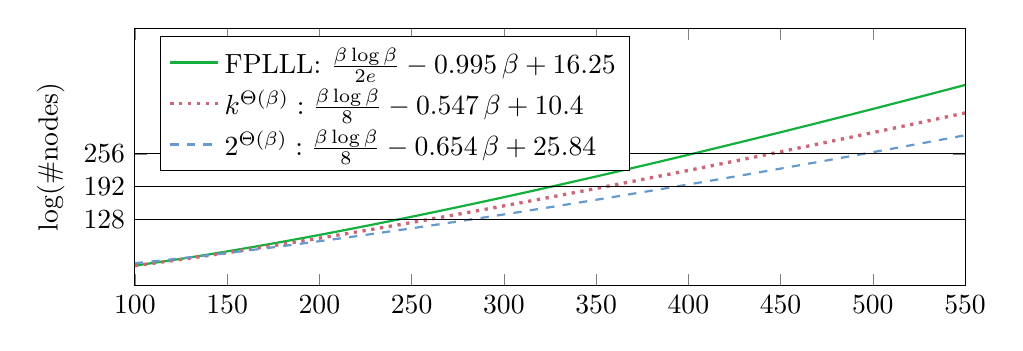
\begin{tikzpicture}
  \begin{axis}[
    legend pos = north west, 
    xmin=100, xmax=550,
    ymin=0, ymax=500,
    height=0.4\textwidth,
    ylabel = \(\log(\#\textnormal{nodes})\),
    ytick = {128,192,256},
    ]
    \addplot+ [domain=100:550, samples=250]{0.1839*x*log2(x) - 0.995*x + 16.25};
    \addlegendentry{FPLLL: \(\frac{\beta \log \beta}{2e} - 0.995\,\beta + 16.25\)};

    \addplot+ [domain=100:550, samples=250]{0.125*x*log2(x) - 0.547*x+10.4};
    \addlegendentry{\(k^{\Theta(\beta)}: \frac{\beta \log \beta}{\alert{8}} - 0.547\,\beta + 10.4\)};

    \addplot+ [domain=100:550,samples=250]{0.125*x*log2(x) - 0.654*x+25.84};
    \addlegendentry{\(2^{\Theta(\beta)}: \frac{\beta \log \beta}{8} - \alert{0.654}\,\beta + 25.84\)};

    \addplot+ [domain=100:550, samples=200, solid, thin,draw=black]{128};
    \addplot+ [domain=100:550, samples=200, solid, thin,draw=black]{192};
    \addplot+ [domain=100:550, samples=200, solid, thin,draw=black]{256};
  \end{axis}
\end{tikzpicture}
\tikzset{external/export=false}

\footnotesize \fullcite{C:ABLR21}
\end{frame}

\begin{frame}[label={sec:org77e81c2}]{Sieving: Key Idea I}
\tikzset{external/export=true}
\tikzsetnextfilename{sieving-idea-1}
\centering
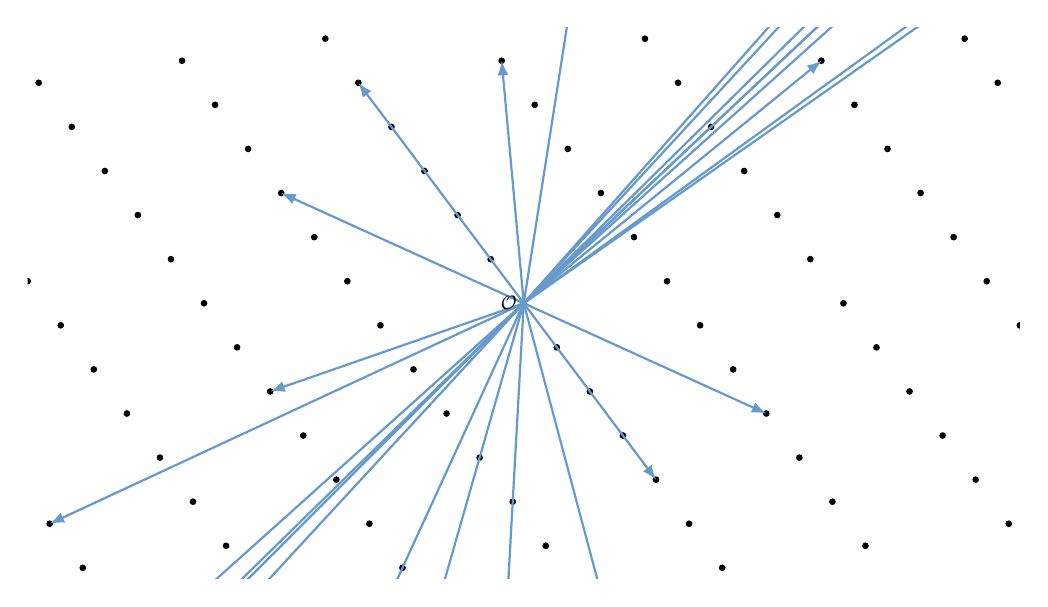
\begin{tikzpicture}[scale=0.7, every node/.style={scale=0.7}]
  \coordinate (Origin)   at (0,0);

  \clip (-9,-5) rectangle (9,5);
  \pgftransformcm{1}{0.6}{0.7}{1}{\pgfpoint{0cm}{0cm}}

  \foreach \x in {-10,-9,...,10}{%
    \foreach \y in {-10,-9,...,10}{%
      \node[draw,circle,inner sep=1pt,fill] at (2*\x,2*\y) {};
    }
  }
  % \draw [ultra thick,-latex,red] (Origin)
  % -- (Bone) node [above left] {$b_1$};
  % \draw [ultra thick,-latex,red] (Origin)
  % -- (Btwo) node [below right] {$b_2$};

  \foreach \x in {-5,-3,2,4,5}{%
    \foreach \y in {-6,-4,1,4,5}{%
      \draw [thick,-latex,DarkBlue] (Origin)
      -- (2*\x,2*\y) {};
    }
  }

  \node [left] at (Origin) {$\mathcal{O}$};
\end{tikzpicture}
\tikzset{external/export=false}
\end{frame}

\begin{frame}[label={sec:orge452407}]{Sieving: Key Idea II}
\tikzset{external/export=true}
\tikzsetnextfilename{sieving-idea-2}
\centering
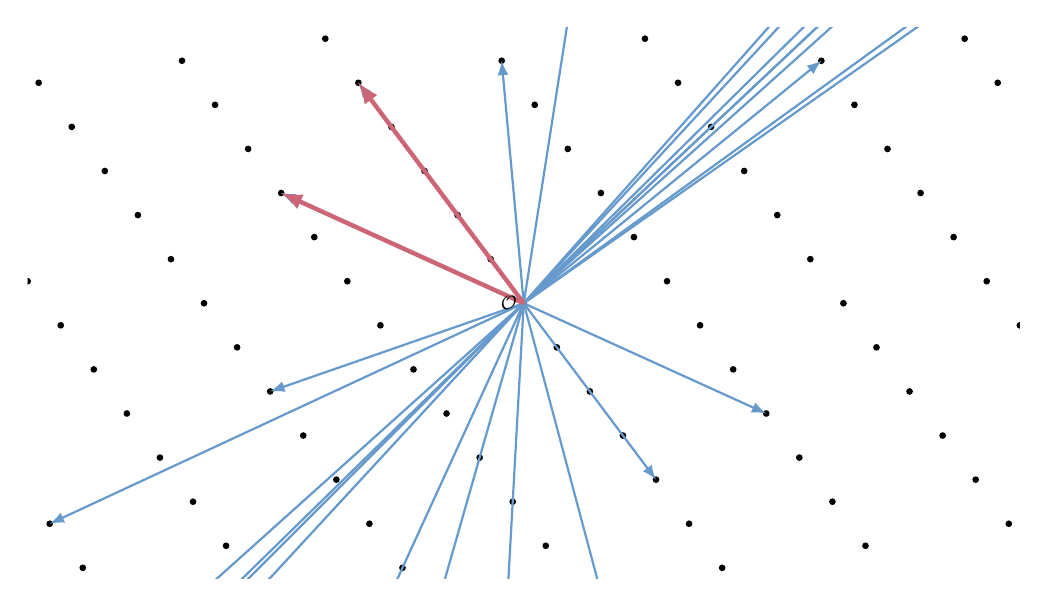
\begin{tikzpicture}[scale=0.7, every node/.style={scale=0.7}]
  \coordinate (Origin)   at (0,0);

  \clip (-9,-5) rectangle (9,5);
  \pgftransformcm{1}{0.6}{0.7}{1}{\pgfpoint{0cm}{0cm}}

  \foreach \x in {-10,-9,...,10}{%
    \foreach \y in {-10,-9,...,10}{%
      \node[draw,circle,inner sep=1pt,fill] at (2*\x,2*\y) {};
    }
  }

  \foreach \x in {-5,-3,2,4,5}{%
    \foreach \y in {-6,-4,1,4,5}{%
      \draw [thick,-latex,DarkBlue] (Origin)
      -- (2*\x,2*\y) {};
    }
  }

  \draw [ultra thick,-latex,LightRed] (Origin) -- (-10,10) {};
  \draw [ultra thick,-latex,LightRed] (Origin) -- (-10,8) {};

  \node [left] at (Origin) {$\mathcal{O}$};
\end{tikzpicture}
\tikzset{external/export=false}
\end{frame}

\begin{frame}[label={sec:orge0381f0}]{Sieving: Key Idea III}
\tikzset{external/export=true}
\tikzsetnextfilename{sieving-idea-3}
\centering
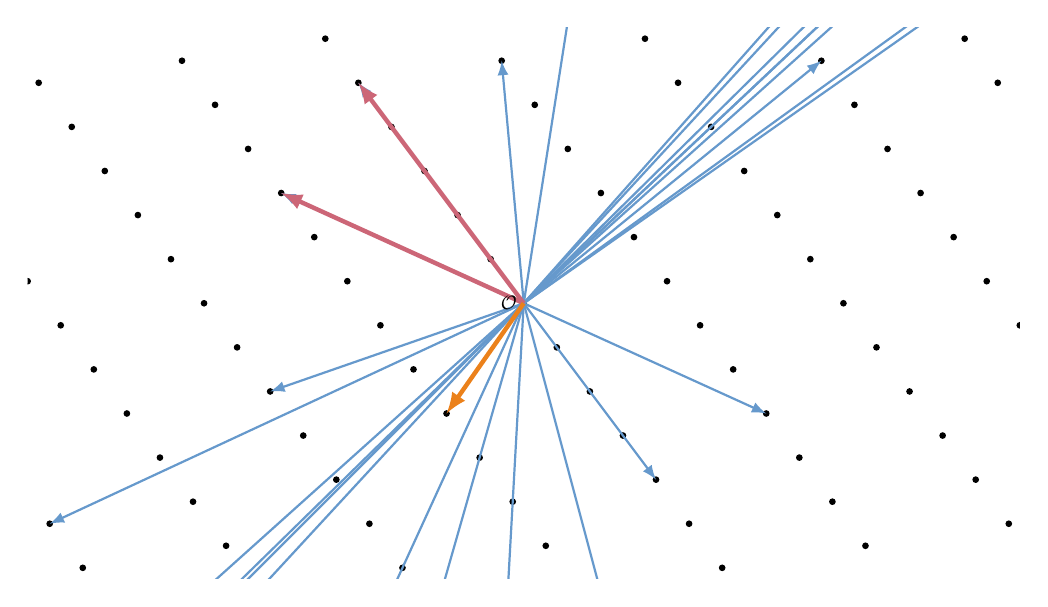
\begin{tikzpicture}[scale=0.7, every node/.style={scale=0.7}]
  \coordinate (Origin)   at (0,0);

  \clip (-9,-5) rectangle (9,5);
  \pgftransformcm{1}{0.6}{0.7}{1}{\pgfpoint{0cm}{0cm}}

  \coordinate (Bone) at (0,2);
  \coordinate (Btwo) at (2,-2);

  \foreach \x in {-10,-9,...,10}{%
    \foreach \y in {-10,-9,...,10}{%
      \node[draw,circle,inner sep=1pt,fill] at (2*\x,2*\y) {};
    }
  }

  \foreach \x in {-5,-3,2,4,5}{%
    \foreach \y in {-6,-4,1,4,5}{%
      \draw [thick,-latex,DarkBlue] (Origin)
      -- (2*\x,2*\y) {};
    }
  }

  \draw [ultra thick,-latex,LightRed] (Origin) -- (-10,10) {};
  \draw [ultra thick,-latex,LightRed] (Origin) -- (-10,8) {};
  \draw [ultra thick,-latex,LightBrown] (Origin) -- (0,-2) {};

  \node [left] at (Origin) {$\mathcal{O}$};
\end{tikzpicture}
\tikzset{external/export=false}
\end{frame}

\begin{frame}[label={sec:orgceca2ef}]{Sieving: Basic (Gauss) Sieve Complexity}
\begin{itemize}
\item Assume all vectors have (roughly) the same length
\item Normalise to unit sphere \(\mathcal{S}^{d-1} \coloneqq \{\vec{x} \in \RR^{d} | \|\vec{x}\| = 1\}\)
\item We have \(\|\vec{v} - \vec{w}\| \leq 1\) iff \(\left\langle \vec{v}, \vec{w} \right\rangle \ge 1/2 = \cos(\pi/3)\)
\item The probability that two random \(\vec{v}, \vec{w} \in \mathcal{S}^{d-1}\) satisfy \(\left\langle \vec{v}, \vec{w} \right\rangle \ge 1/2\) is
\[\frac{1}{\sqrt{\pi}} \cdot \frac{\Gamma(d/2)}{\Gamma((d-1)/2)} \cdot \int_{0}^{\pi/3} \sin^{d-2}(x)\, \mathsf{d}x = \poly[d] \cdot {\left(\frac{4}{3}\right)}^{d/2} \approx 2^{0.2075\,d + o(d)}\]
\item Need \(\poly[d] \cdot {\left(\frac{4}{3}\right)}^{d/2}\) vectors, comparing all pairs costs \(\poly[d] \cdot {\left(\frac{4}{3}\right)}^{d} \approx 2^{0.4150\,d + o(d)}\).
\end{itemize}


\footnotesize \fullcite{SODA:MicVou10}
\end{frame}

\begin{frame}[label={sec:org7430d8a}]{Sieving: Buckets I}
\tikzset{external/export=true}
\tikzsetnextfilename{sieving-buckets}
\centering
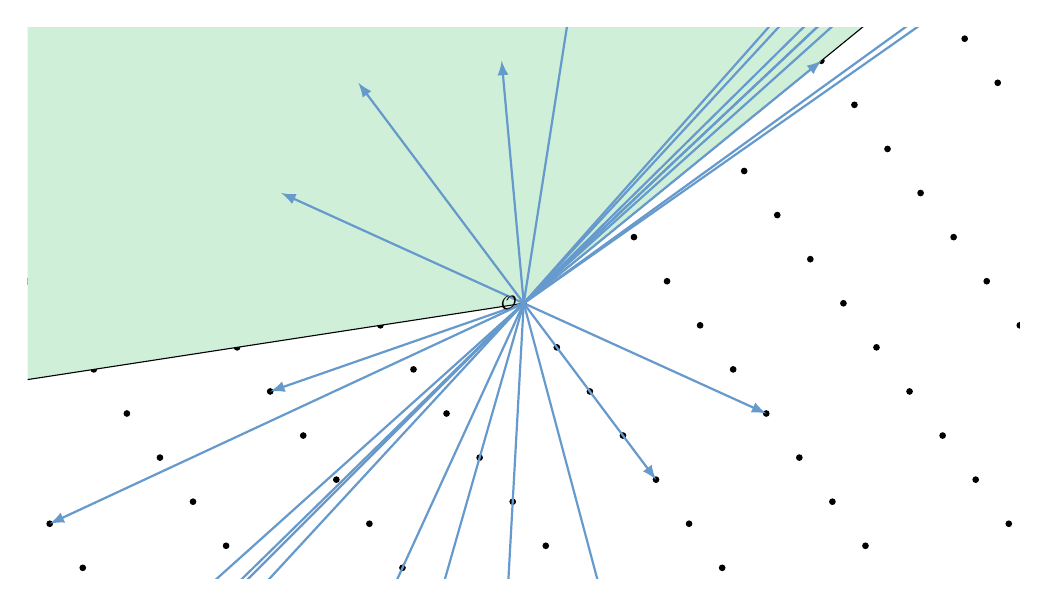
\begin{tikzpicture}[scale=0.7, every node/.style={scale=0.7}]
  \coordinate (Origin)   at (0,0);

  \clip (-9,-5) rectangle (9,5);
  \pgftransformcm{1}{0.6}{0.7}{1}{\pgfpoint{0cm}{0cm}}

  \coordinate (Bone) at (0,2);
  \coordinate (Btwo) at (2,-2);

  \foreach \x in {-10,-9,...,10}{%
    \foreach \y in {-10,-9,...,10}{%
      \node[draw,circle,inner sep=1pt,fill] at (2*\x,2*\y) {};
    }
  }

\draw[fill=LightGreen!20!white] (-20,10) -- (0,0) -- (20,10) -- (-100,100) {};

\foreach \x in {-5,-3,2,4,5}{%
    \foreach \y in {-6,-4, 1,4,5}{%
      \draw [thick,-latex,DarkBlue] (Origin)
      -- (2*\x,2*\y) {};
    }
 }

  \node [left] at (Origin) {$\mathcal{O}$};
\end{tikzpicture}
\tikzset{external/export=false}
\end{frame}

\begin{frame}[label={sec:orgcddeaf7}]{Sieving: Buckets II}
If \(\vec{v}\), \(\vec{c}\) are somewhat close and \(\vec{w}\), \(\vec{c}\) are somewhat close then perhaps \(\vec{w}\), \(\vec{v}\) are close?

\begin{block}{Strategy}
\begin{itemize}
\item Sort vectors into somewhat loose buckets,
\item Do quadratic pairwise comparison only within each bucket.
\end{itemize}
\end{block}

\begin{description}
\item[{BGJ}] Split search space into buckets. \textbf{Cost}: \(2^{0.311\,\beta + o(\beta)}\).\footfullcite{EPRINT:BecGamJou15}
\item[{BDGL}] Use codes to decide which bucket to consider. \textbf{Cost}: \(2^{0.292\,\beta + o(\beta)}\). \footfullcite{SODA:BDGL16}
\end{description}
\end{frame}

\begin{frame}[label={sec:orgbb544fc}]{Sieving: Popcount I}
\tikzset{external/export=true}
\tikzsetnextfilename{sieving-popcount-1}
\centering
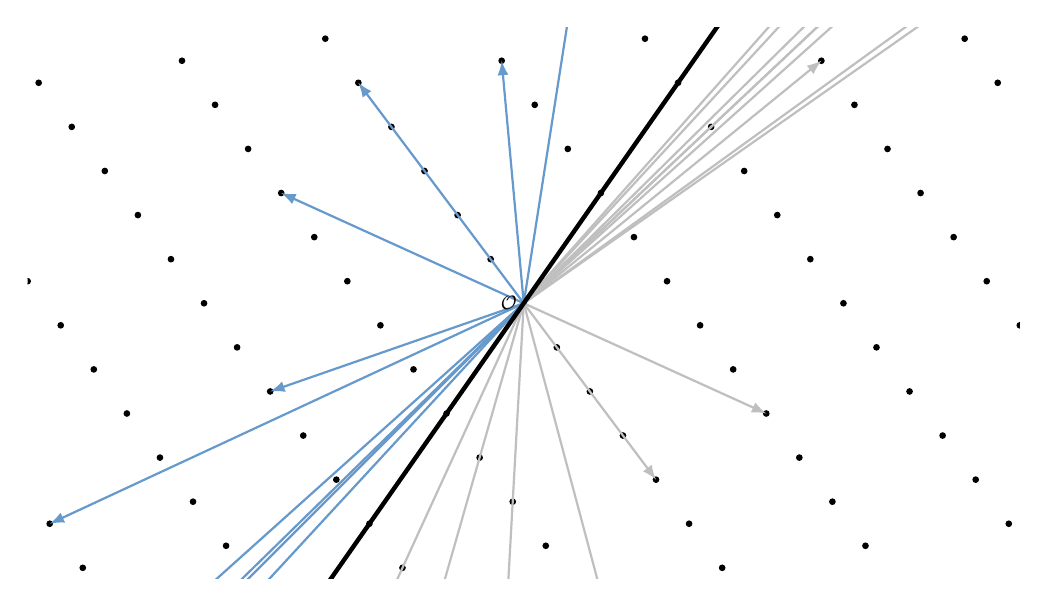
\begin{tikzpicture}[scale=0.7, every node/.style={scale=0.7}]
  \coordinate (Origin)   at (0,0);

  \clip (-9,-5) rectangle (9,5);
  \pgftransformcm{1}{0.6}{0.7}{1}{\pgfpoint{0cm}{0cm}}

  \coordinate (Bone) at (0,2);
  \coordinate (Btwo) at (2,-2);

  \foreach \x in {-10,-9,...,10}{%
    \foreach \y in {-10,-9,...,10}{%
      \node[draw,circle,inner sep=1pt,fill] at (2*\x,2*\y) {};
    }
  }

  \foreach \x in {2,4,5}{%
    \foreach \y in {-6,-4,1,4,5}{%
      \draw [thick,-latex,lightgray] (Origin)
      -- (2*\x,2*\y) {};
    }
  }


  \foreach \x in {-5,-3}{%
    \foreach \y in {-6,-4,1,4,5}{%
      \draw [thick,-latex,DarkBlue] (Origin)
      -- (2*\x,2*\y) {};
    }
  }
  \draw[ultra thick] (0,-10) -- (0,10);

  \node [left] at (Origin) {$\mathcal{O}$};
\end{tikzpicture}
\tikzset{external/export=false}
\end{frame}

\begin{frame}[label={sec:orgd61fc55}]{Sieving: Popcount II}
Most comparisons result in a "no" answer, rejecting those pairs quickly improves performance, even if we lose a few good pairs.

\begin{itemize}
\item For a given plane, denote a vector being on the “left” as 0, being on the “right” as 1.
\item This defines a 1-bit locality sensitive hash (LSH) function.
\item Consider many such hash functions and concatenate their output.
\item Two vectors are close if they agree on many bits of their hashes
\end{itemize}

\begin{block}{Comparison Operation}
XOR hash values and compute Hamming weight (“popcount”).
\end{block}
\end{frame}

\begin{frame}[label={sec:org522cf63}]{Sieving: G6K}
G6K \footfullcite{EC:ADHKPS19} is a Python/C++ framework for experimenting with sieving algorithms (inside and outside BKZ)
\begin{itemize}
\item Does not take the “oracle” view but considers sieves as stateful machines.
\item Implements several sieve algorithms
\begin{itemize}
\item Gauss and NV
\item Triple Sieve
\item BGJ1 (BGJ with one level of filtration)
\item BDGL (with one and two block respectively)
\end{itemize}
\item Applies recent tricks and adds new tricks for improving performance of sieving
\end{itemize}
\end{frame}

\begin{frame}[label={sec:orgd676f11}]{Sieving: SVP}
\begin{center}
\begin{tikzpicture}
    \begin{semilogyaxis}[ylabel=seconds, xlabel=\(\beta\), legend style={fill=}, legend pos=north west, height=0.5\textwidth]
        \addplot+ [only marks] table [x=d, y=FPLLL, col sep=comma]{data/exact-svp.csv};
        \addlegendentry{BKZ + pruned enum (FPLLL)};
        \addplot+ [only marks] table [x=d, y=G6K, col sep=comma]{data/exact-svp.csv};
        \addlegendentry{G6K WorkOut};
    \end{semilogyaxis}
\end{tikzpicture}
Average time in seconds for solving exact SVP
\end{center}
\end{frame}

\begin{frame}[label={sec:org8f2bf2f}]{Darmstadt HSVP\textsubscript{1.05} Challenges}
\begin{center}
\begin{tikzpicture}
  \begin{axis}[xlabel=\(d\),ylabel=\(\log_2(\textnormal{cycles})\),height=0.5\textwidth]
    \addplot table [x=d, col sep=comma, y expr = log2(100*\thisrowno{2}),, select coords between index={0}{50} ]{data/fplll-simulations,svp-challenge.csv};
    \addlegendentry{HSVP\(_{1.05}\) non-parallel enum sim};

    \addplot table [x=d, col sep=comma, y expr = log2(100*\thisrowno{2}), select coords between index={70}{166}]{data/fplll-simulations-enumeration-cost-2e.csv};
    \addlegendentry{SVP non-parallel enum sim};

    \addplot+ [only marks] table [unbounded coords=discard,x=d, col sep=comma, y expr = %
    log2(\thisrowno{3}*3600*2*10.0^9)%
    ]{data/svp-challenge-observations.csv};
    \addlegendentry{HoF:FK15};

    \addplot+ [only marks] table [unbounded coords=discard,x=d, col sep=comma, y expr = %
    log2(\thisrowno{4}*3600*2*10.0^9)%
    ]{data/svp-challenge-observations.csv};
    \addlegendentry{HoF:KT17};

    \addplot+ [only marks] table [unbounded coords=discard,x=d, col sep=comma, y expr = %
    log2(\thisrowno{5}*3600*2*10.0^9)%
    ]{data/svp-challenge-observations.csv};
    \addlegendentry{G6K};

  \end{axis}
\end{tikzpicture}
\end{center}
\end{frame}

\begin{frame}[label={sec:orgc959e91}]{GPU Sieving}
\begin{itemize}
\item Stream database of vectors to GPU
\item Run low precision inner products there in the spirit of popcount
\end{itemize}

\begin{center}
\begin{tabular}{rrrrrrrrr}
\toprule
dim & TD4F & D4F & MSD & Norm & Norm/GH & FLOP & Walltime & Mem GiB\\
\midrule
158 & 31 & 29 & 129 & 3303 & 1.04329 & 262.1 & 9h 16m & 89\\
162 & 31 & 31 & 131 & 3341 & 1.04220 & 263.2 & 18h 32m & 156\\
176 & 34 & 33 & 143 & 3487 & 1.04412 & 267.5 & 12d 11h & 806\\
178 & 34 & 32 & 146 & 3447 & 1.02725 & 268.6 & 22d 18h & 1060\\
180 & 34 & 30 & 150 & 3509 & 1.04003 & 269.9 & 51d 14h & 1443\\
\bottomrule
\end{tabular}

\end{center}

\scriptsize

\fullcite{EC:DucSteWoe21}
\end{frame}

\begin{frame}[label={sec:orge0847ac},fragile]{Try it at Home}
 \lstset{language=sage,label= ,caption= ,captionpos=b,numbers=none}
\begin{lstlisting}
from fpylll import IntegerMatrix, GSO, LLL
from fpylll.tools.bkz_stats import dummy_tracer
from g6k import Siever
from g6k.algorithms.bkz import pump_n_jump_bkz_tour

A = LLL.reduction(IntegerMatrix.random(180, "qary", k=90, bits=20))
g6k = Siever(A)

for b in range(20, 60+1, 10):
    pump_n_jump_bkz_tour(g6k, dummy_tracer, b, pump_params={"down_sieve": True})
\end{lstlisting}

\begin{description}
\item[{\url{https://github.com/fplll/g6k}}] C++ kernel + Python frontend
\item[{\url{https://github.com/WvanWoerden/G6K-GPU-Tensor}}] G6K fork adding GPU support
\end{description}
\end{frame}

\begin{frame}[label={sec:org64cdffc}]{Details Matter}
\begin{columns}[t]
\begin{column}{0.5\columnwidth}
"\emph{The main difference is the cost of the random product code decoding algorithm. Our algorithm requires one addition, one xor, and three comparisons per legal codeword, which translate to 433 gates for a lattice of rank 400, as opposed to [AGPS20] which requires a super-constant number of inner products per legal codeword, which translate to 3,540,524 gates for a lattice of rank 400.}"

\ \\
\scriptsize

\fullcite{Matzov2022}
\end{column}

\begin{column}{0.5\columnwidth}
"\emph{Concretely, we conclude on an overhead factor of about  on the number of gates in the RAM model compared to the idealized model for dimensions around  after an appropriate re-parametrization. Part of this overhead can be traded for extra memory, at a costly rate.}"

\ \\
\scriptsize

\fullcite{EPRINT:Ducas22}
\end{column}
\end{columns}
\end{frame}

\section{Quantum Stuff}
\label{sec:org8491de5}
\begin{frame}[label={sec:orgff1cdf3}]{Quantum Estimates}
\begin{description}
\item[{{\color{LightRed} \textbf{Sieving} }}] Given some vector \(\vec{w}\) and a list of vectors \(L\), apply Grover’s algorithm to find \(\{\vec{v} \in L \textnormal{ s.t. } \|\vec{v} \pm \vec{w}\| \leq \|\vec{w}\|\}\).\footfullcite{PhD:Laarhoven15}

\item[{{\color{DarkBlue} \textbf{Enumeration} }}] Apply Montanaro’s quantum backtracking algorithm for quadratic speed-up.\footfullcite{EPRINT:AonNguShe18}
\end{description}
\end{frame}

\begin{frame}[label={sec:org2d3e741}]{Quantum Sieving}
\begin{itemize}
\item A quantum sieve needs list of \(2^{0.2075 \beta}\) vectors before pairwise search with Grover

\item Fast sieves use that the search is structured, Grover does unstructured search
\begin{itemize}
\item Quantum Gauss Sieve \[2^{(0.2075 + \frac{1}{2} 0.2075)\, \beta + o(\beta)} = 2^{0.311\, \beta + o(\beta)} \textnormal{ time},\qquad 2^{0.2075\, \beta + o(\beta)} \textnormal{ memory}\]
\item Classical BGJ Sieve \footfullcite{EPRINT:BecGamJou15} \[\phantom{2^{(0.2075 + \frac{1}{2} 0.2075)\, \beta + o(\beta)} = }2^{0.311\, \beta + o(\beta)}\textnormal{ time}, \qquad 2^{0.2075\, \beta + o(\beta)} \textnormal{ memory}\]
\end{itemize}
\item Asymptotically fastest sieves have small lists and thus less Grover speed-up potential
\end{itemize}
\end{frame}

\begin{frame}[label={sec:orga44873e}]{Implementing Quantum Algorithms for SVP}
\begin{columns}[t]
\begin{column}{0.5\columnwidth}
\textbf{Sieving}

\begin{itemize}
\item Major operation is to check whether two vectors reduce to some smaller vector
\item Can be implemented using the XOR and popcount trick \(\Rightarrow\) the quantum circuit is relatively small.
\item Sieving requires exponentially large quantum accessible RAM (qRAM). Not clear that this can be built efficiently (due to error correction being required).
\end{itemize}
\end{column}

\begin{column}{0.5\columnwidth}
\textbf{Enumeration}

\begin{itemize}
\item Enumeration requires higher precision floating point arithmetic.
\item Quantum circuit for enumeration is likely to be larger than for sieving.
\item But no exponential qRAM.
\end{itemize}
\end{column}
\end{columns}
\end{frame}

\begin{frame}[label={sec:orgfe5c5af}]{Implementing Quantum Algorithms for SVP: Sieving}
\begin{center}
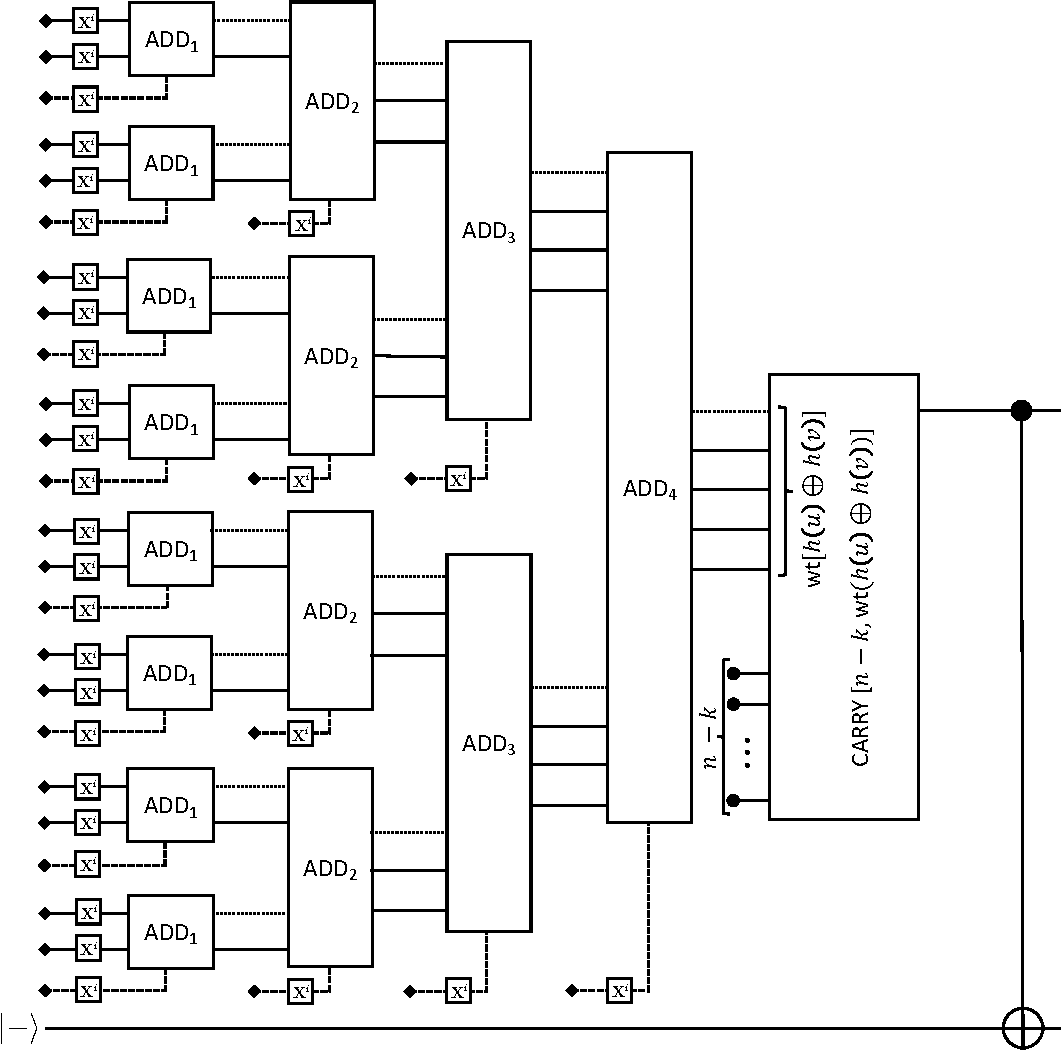
\includegraphics[width=0.5\textwidth]{./popcount-quantum-circuit.pdf}
\end{center}
\end{frame}

\begin{frame}[label={sec:orge443022}]{Implementing Quantum Algorithms for SVP: Sieving (Underestimates)}
\tikzset{external/export=true}
\tikzsetnextfilename{quantum-sieving-bdgl-ge}
\tikzpicturedependsonfile{data/cost-estimate-list_decoding-classical.csv}
\tikzpicturedependsonfile{data/cost-estimate-list_decoding-ge19.csv}
\begin{tikzpicture}
  \begin{axis}[ylabel={$\log_{2}(\#ops)$}, height=0.5\textwidth,xlabel=,]
    \addplot+[] table [x=d, col sep=comma, y=log_cost] {data/cost-estimate-list_decoding-classical.csv};
    \addlegendentry{BDGL (c: RAM)};

    \addplot+[] [domain=64:1024] {0.2924*x};
    \addlegendentry{\(0.2924\,d\)};

    \addplot+[] table [x=d, col sep=comma, y=log_cost] {data/cost-estimate-list_decoding-ge19.csv};
    \addlegendentry{BDGL (q: Gidney and Ekerå 2019)};

    \addplot+[] [domain=64:1024] {0.2652*x};
    \addlegendentry{\(0.2652\,d\)};
  \end{axis}
\end{tikzpicture}
\tikzset{external/export=false}


\scriptsize{

\fullcite{EPRINT:AGPS19}

}
\end{frame}

\begin{frame}[label={sec:orgf233f5f}]{Quantum Algorithms Open Problems}
\begin{itemize}
\item A quantum circuit for enumeration.
\item Better algorithms than best classical + Grover?
\item Near-term noisy quantum computers?
\item Quantum improvements on a higher level?
\end{itemize}
\end{frame}

\begin{frame}[label={sec:org6cee553}]{Other Approaches}
\begin{description}
\item[{BKW}] combinatorial technique, relatively efficient for small secrets
\item[{Arora-Ge}] use Gröbner bases, asymptotically efficient , but large constants in the exponent
\item[{Hybrid Attack}] combine combinatorial techniques with lattice reduction
\end{description}

\begin{alertblock}{Rule of Thumb}
Don’t need to worry about these unless secret is unusually small (e.g. ternary) and/or sparse.
\end{alertblock}
\end{frame}

\begin{frame}[label={sec:org8154661},standout]{Fin}
\begin{center}
\Huge \alert{Thank You}
\end{center}
\end{frame}

\begin{frame}[allowframebreaks]{References}
\renewcommand*{\bibfont}{\scriptsize}
\printbibliography[heading=none]
\end{frame}
\end{document}